\documentclass[11pt,twocolumn,twoside]{opticajnl}
%% Please use 11pt if submitting to AOP
% \documentclass[11pt,twocolumn,twoside]{opticajnl}

\journal{pr} % Choose journal (ao,jocn,josaa,josab,ol,optica,pr)

%See template introduciton for guidance on setting shortarticle option
\setboolean{shortarticle}{True}
% true = letter/tutorial
% false = research/review article
% (depending on journal)
\usepackage{lineno}
\usepackage[utf8]{inputenc}
\spanishdecimal{.}
\usepackage{amsmath}
\usepackage{caption}
\usepackage{subcaption}
\usepackage[spanish]{babel}
\usepackage{hyperref}
\usepackage{listings}
\usepackage{multicol}
\usepackage[export]{adjustbox}
%\linenumbers
\lstdefinestyle{mystyle}{
    language=Python, % Choose the programming language (e.g., Python)
    basicstyle=\ttfamily, % Set the font style
    keywordstyle=\color{blue}, % Define the color for keywords
    commentstyle=\color{green!40!black}, % Define the color for comments
    numbers=left, % Show line numbers
    numberstyle=\tiny, % Set the style for line numbers
    frame=single, % Add a frame around the code
    breaklines=true, % Allow line breaks within code
    showstringspaces=false % Don't show spaces within strings
}


% Configura el formato del título del listado
\renewcommand\lstlistingname{Código}
\renewcommand\lstlistlistingname{Códigos}
\title{
\vspace{0.1cm} 

Trabajo práctico 1: Imágenes digitales}

\author[1]{\huge{Ignacio Lembo Ferrari}}
\affil[1]{\large{ignaciolembo@ib.edu.ar} 

\vspace{0.1cm}

{\datesfont 1 de marzo del 2024.}

\vspace{0.1cm}
}

%\begin{abstract}
%\textbf{hola}
%\end{abstract}

\begin{document}

\maketitle

\section{Transformaciones de contraste\label{sec:ej1ej2}}

\vspace{0.3cm}

Se tiene una imagen ImagenA.pgm de $181\times217$ pixels de la cual se obtuvo el histograma de intensidades, como se muestra en la Fig. \ref{fig:Semilineartrans}a, y sobre la cual se implementaron diversas transformaciones de contraste. Todas las implementaciones de esta sección se realizaron en python.

En primer lugar, se aplicó una transformación semilinear en los niveles de gris para optimizar el rango dinámico. 

\begin{figure}[h]
    \centering
         \begin{subfigure}[h]{\linewidth}
            \centering
            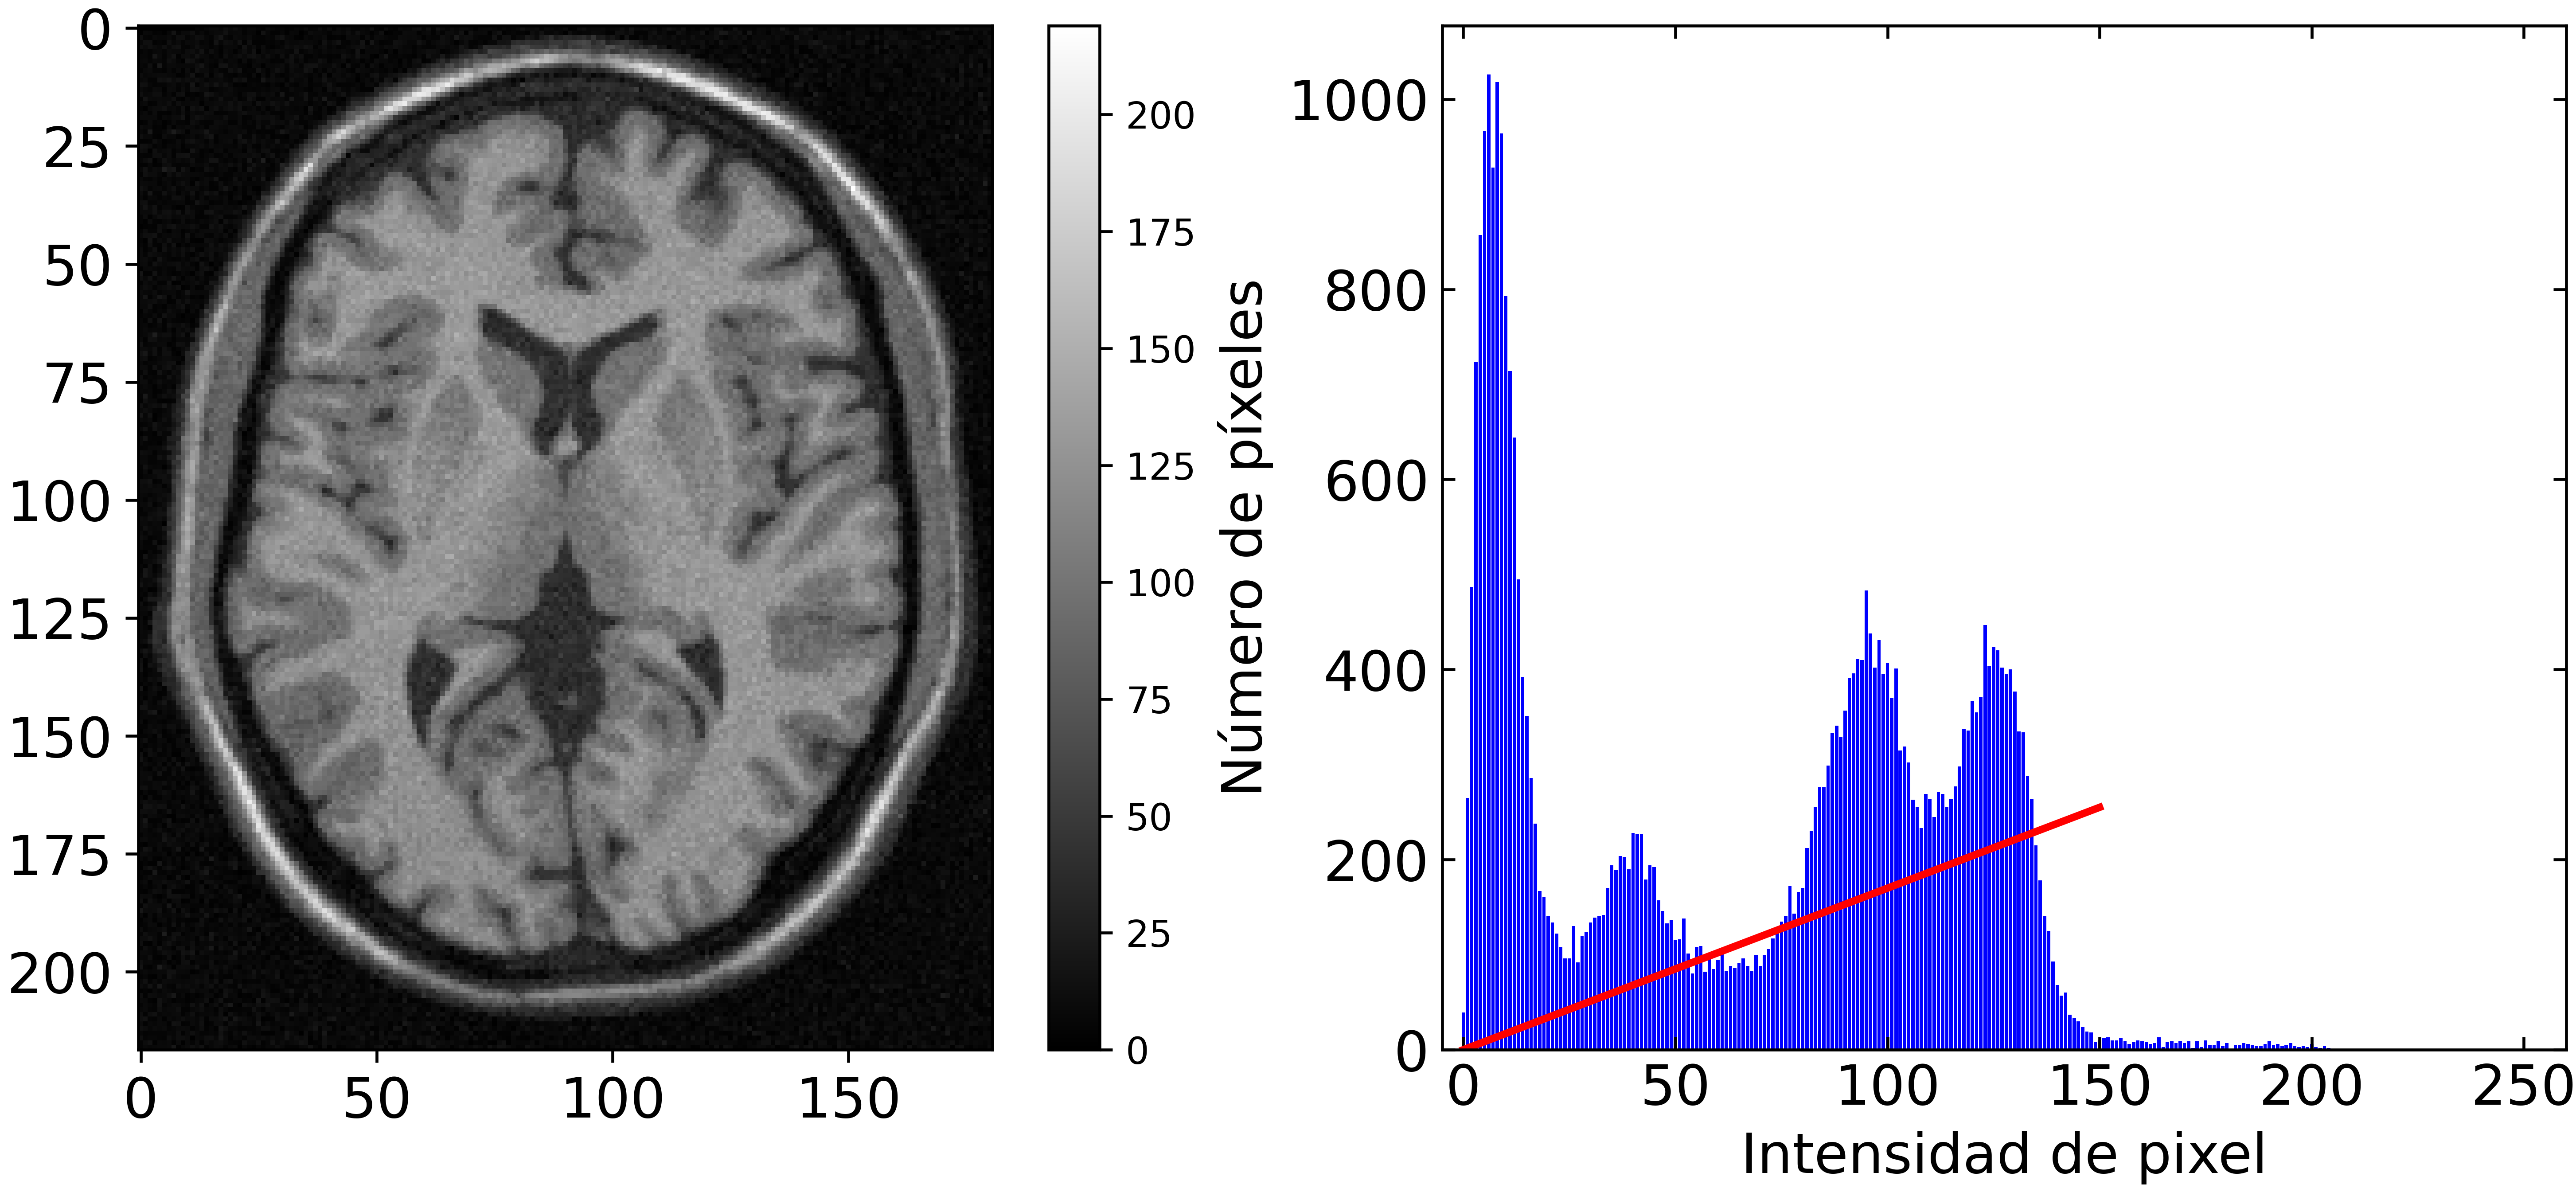
\includegraphics[width=\textwidth]{Figuras/ImageA_brute.png}
            \caption{ImagenA original junto con su histograma de intensidades.} 
         \end{subfigure}
         \begin{subfigure}[h]{\linewidth}
            \centering
            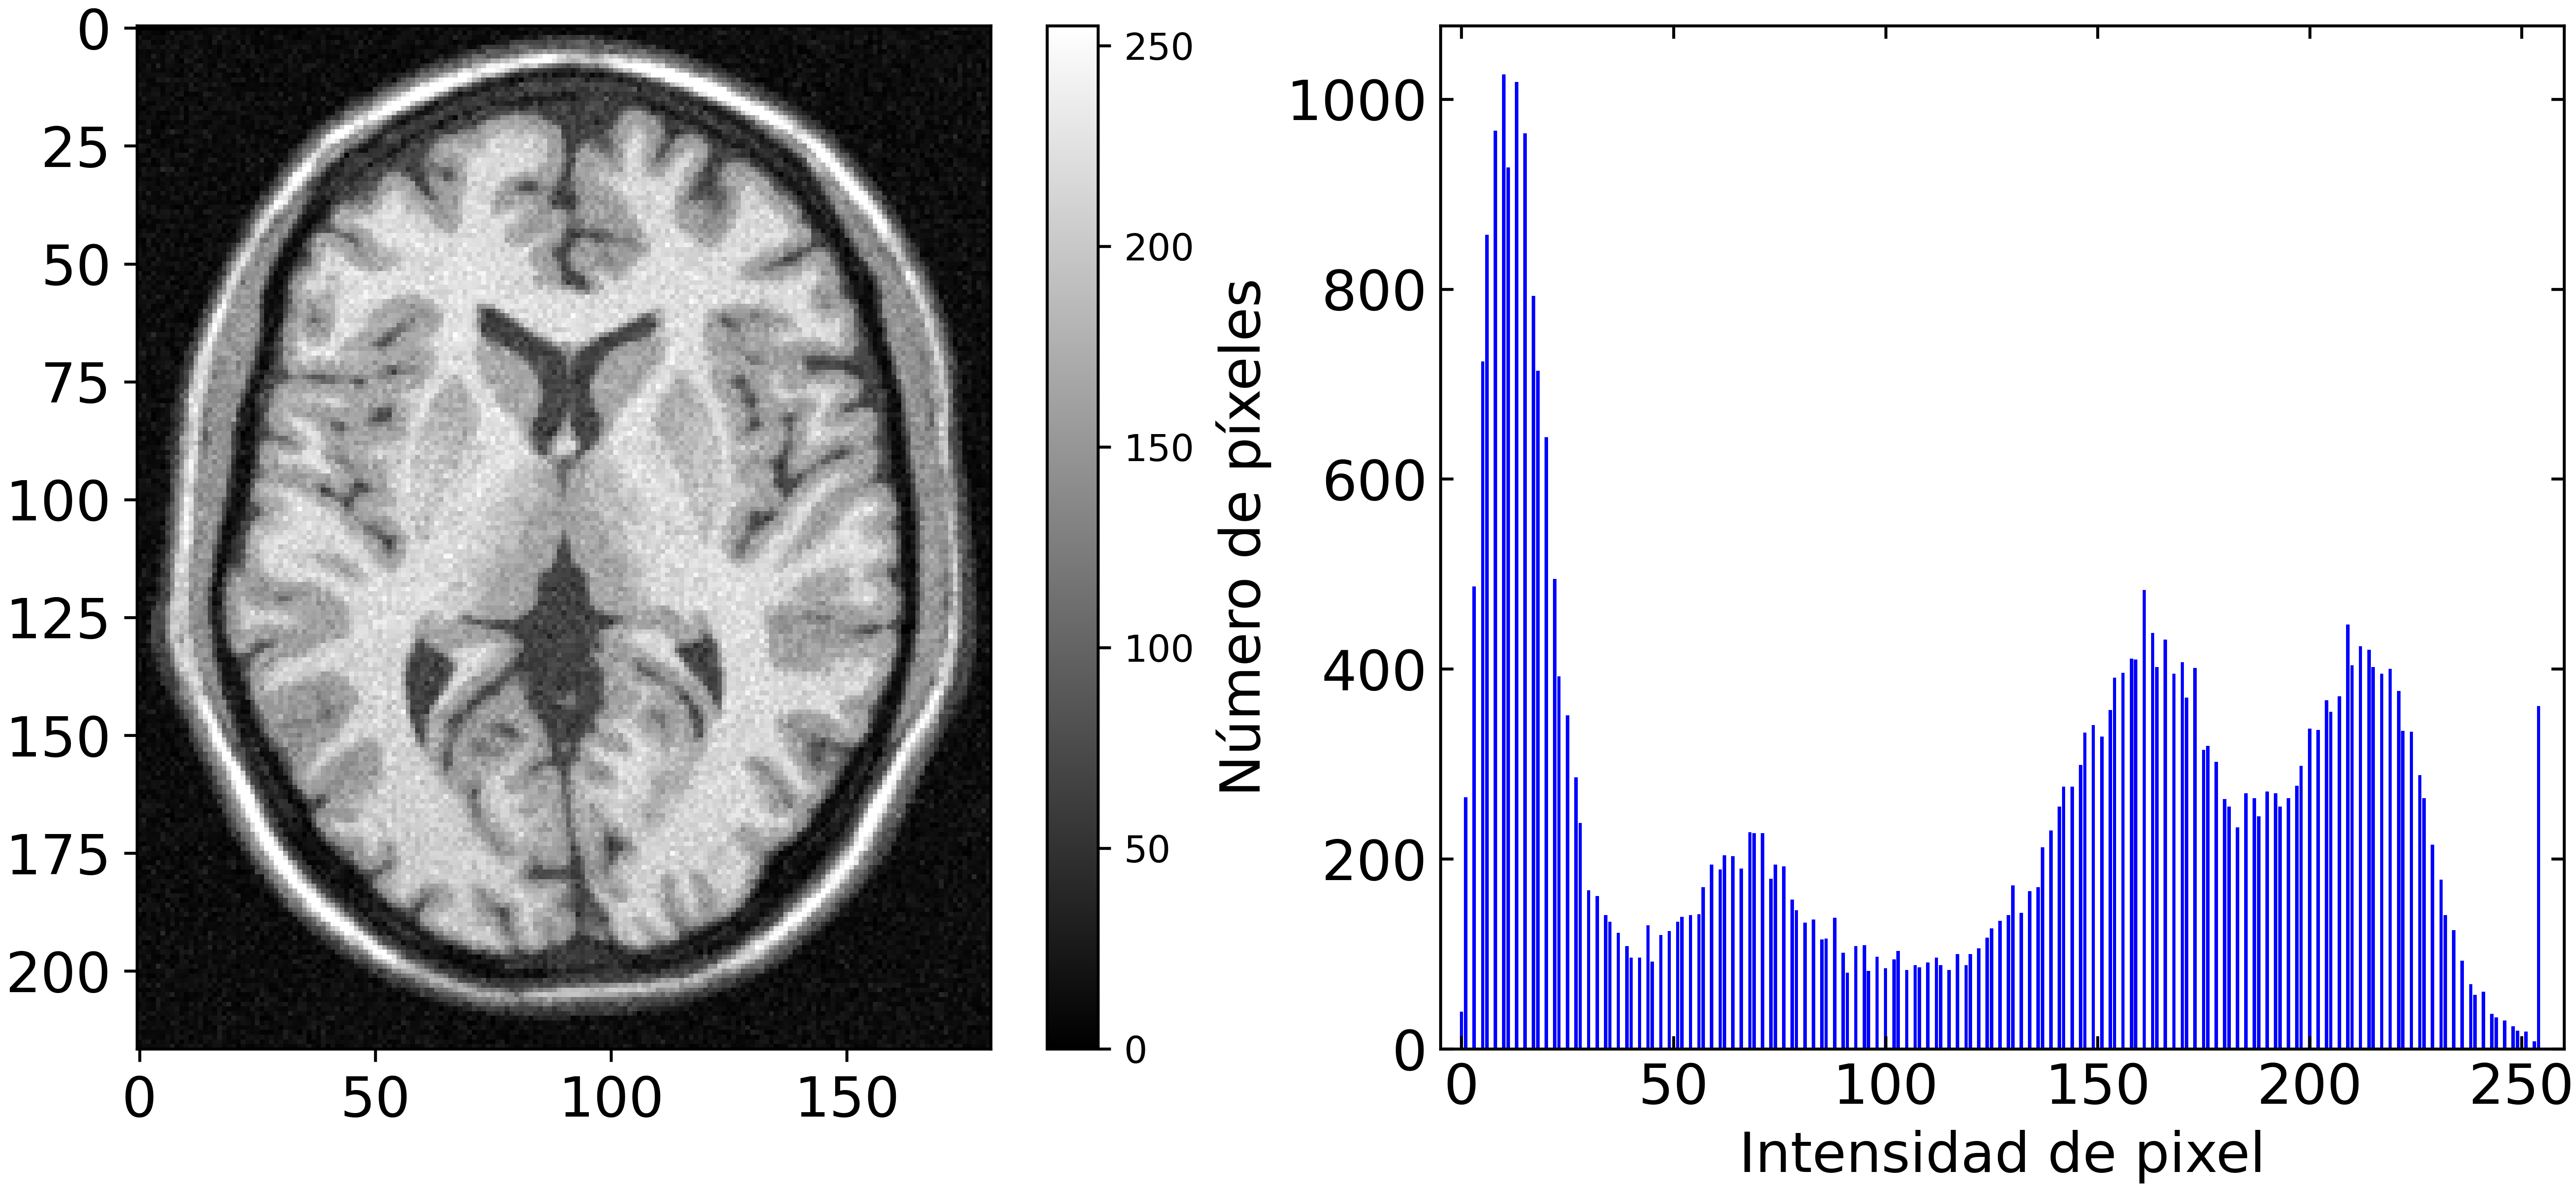
\includegraphics[width=\textwidth]{Figuras/ImageA_0_150.png}
            \caption{ImagenA transformada junto con su histograma de intensidades.}
         \end{subfigure}
    \caption{ImageA original (a) y su transformación semilineal con $r_{min} = 0$ y $r_{min} = 150$ (b), junto con sus correspondientes histogramas de intensidades. Se observa en la imagen transformada que el histograma se corre hacia la derecha y se expande el rango dinámico.}
    \label{fig:Semilineartrans}
\end{figure}

Este método consiste en aplicar una transformación de la forma $T(r) = a r + b$, con $r$ la intensidad del pixel, $a = (I_{max} - I_{min})/(r_{max}-r_{min})$ y $b=I_{min} - ar_{min}$, además
\begin{itemize}
    \item Si $a r + b < I_{min} \Rightarrow T(r)=I_{min}$,
    \item Si $a r + b > I_{max} \Rightarrow T(r)=I_{max}$.
\end{itemize}
Se tomó $I_{min}=0$ e $I_{max}=255$. Para determinar los valores $r_{min}$ y $r_{max}$ de la imagen, se observa, en el histograma de la imagen original, que la mayor cantidad de valores de intensidad se concentran en el rango $[0, 150]$. Luego se toma $r_{min}=0$ y $r_{max}=150$. De esta manera, se obtiene una transformación semilineal que expande el rango dinámico de la imagen. Cabe destacar que los valores por debajo de $I_{min}$ y por encima de $I_{max}$ saturan ne dichos valores, lo cual resulta en pérdida de información de la imagen original. En la Fig. \ref{fig:Semilineartrans}b se observa la transformación semilinear junto con su correspondiente histograma de intensidades. Se observa que el histograma se corre hacia la derecha y se expande el rango dinámico. Podemos ver, en el histograma de la imagen transformada que se acumulan pixeles con intensidad máxima $I_{max}$.

En el histograma de la imagen original se distinguen 4 picos de intensidad, que corresponden 4 regiones de la imagen; De menor a mayor valor de intensidad: Fondo, líquido, materia gris y materia blanca. Se eligieron convenientemente los valores de $r_{min}$ y $r_{max}$ para que la transformación semilinear resalte cada una de estas regiones. El resultado se muestra en la Fig. \ref{fig:Semilineartrans_region}.

\begin{figure}[h]
    \centering
         \begin{subfigure}[h]{0.24\linewidth}
            \centering
            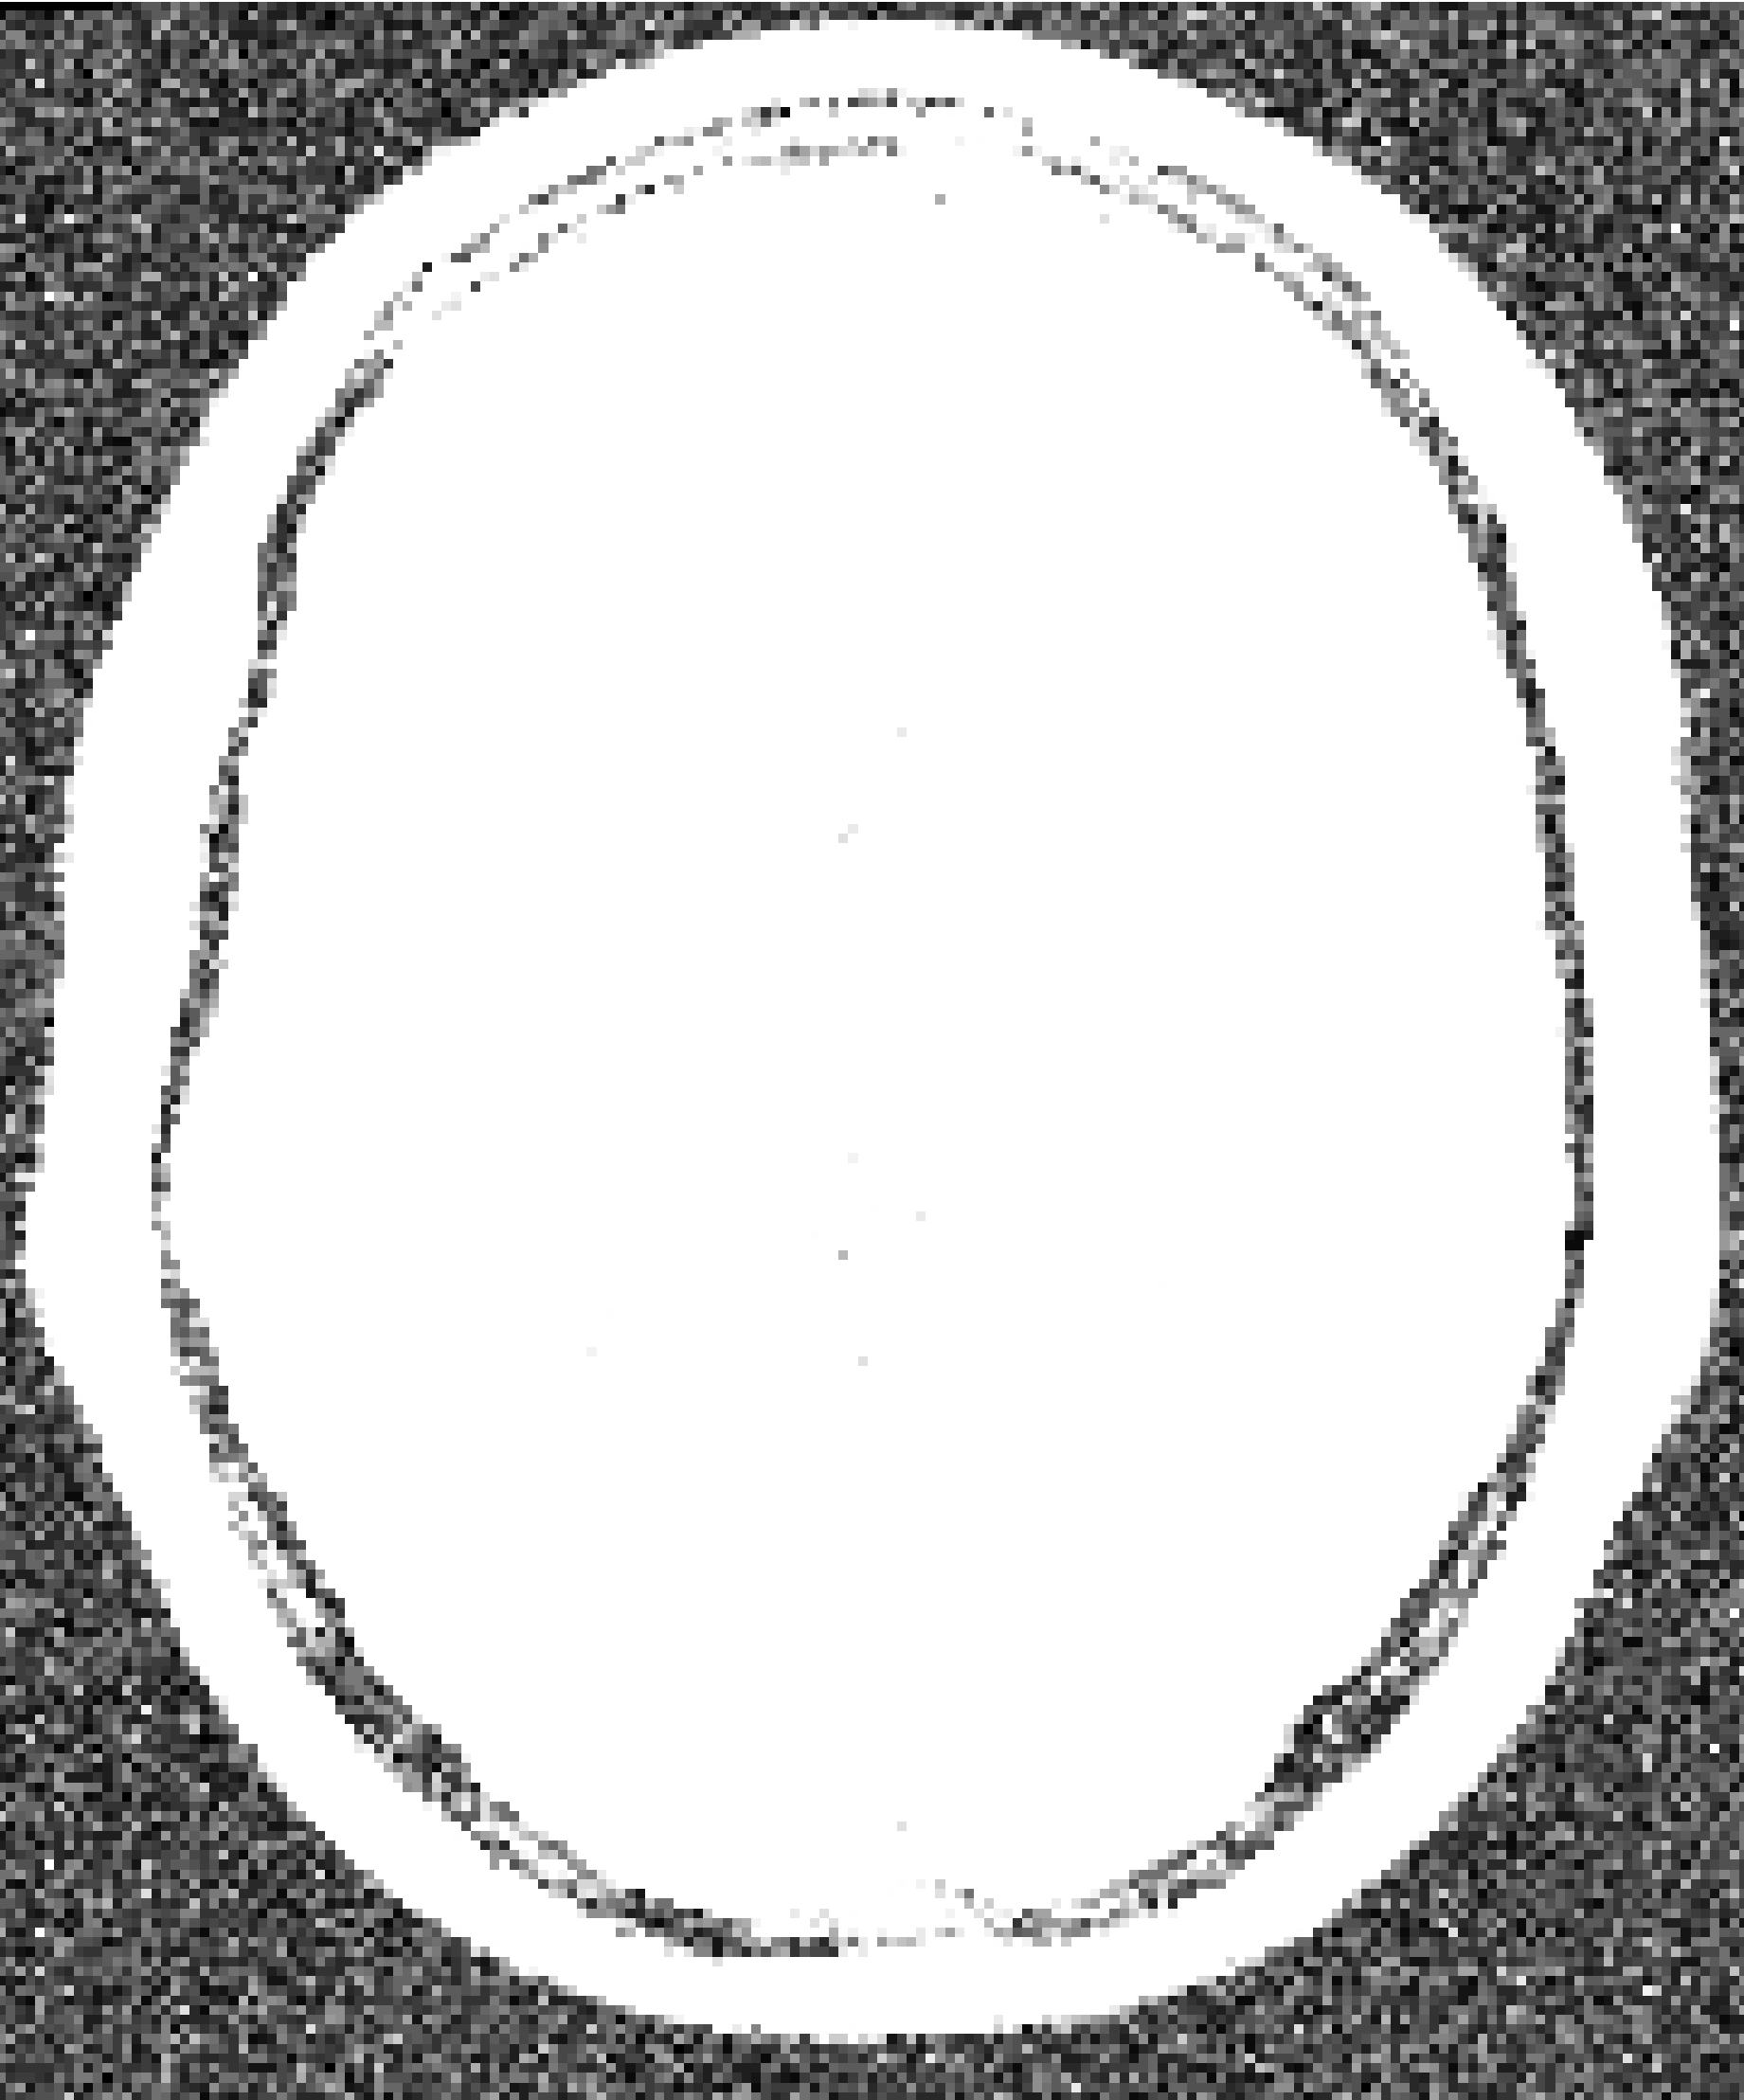
\includegraphics[width=\textwidth]{Figuras/ImageA_0_25.png}
            \caption{Fondo \\
            $~$} 
         \end{subfigure}
         \begin{subfigure}[h]{0.24\linewidth}
            \centering
            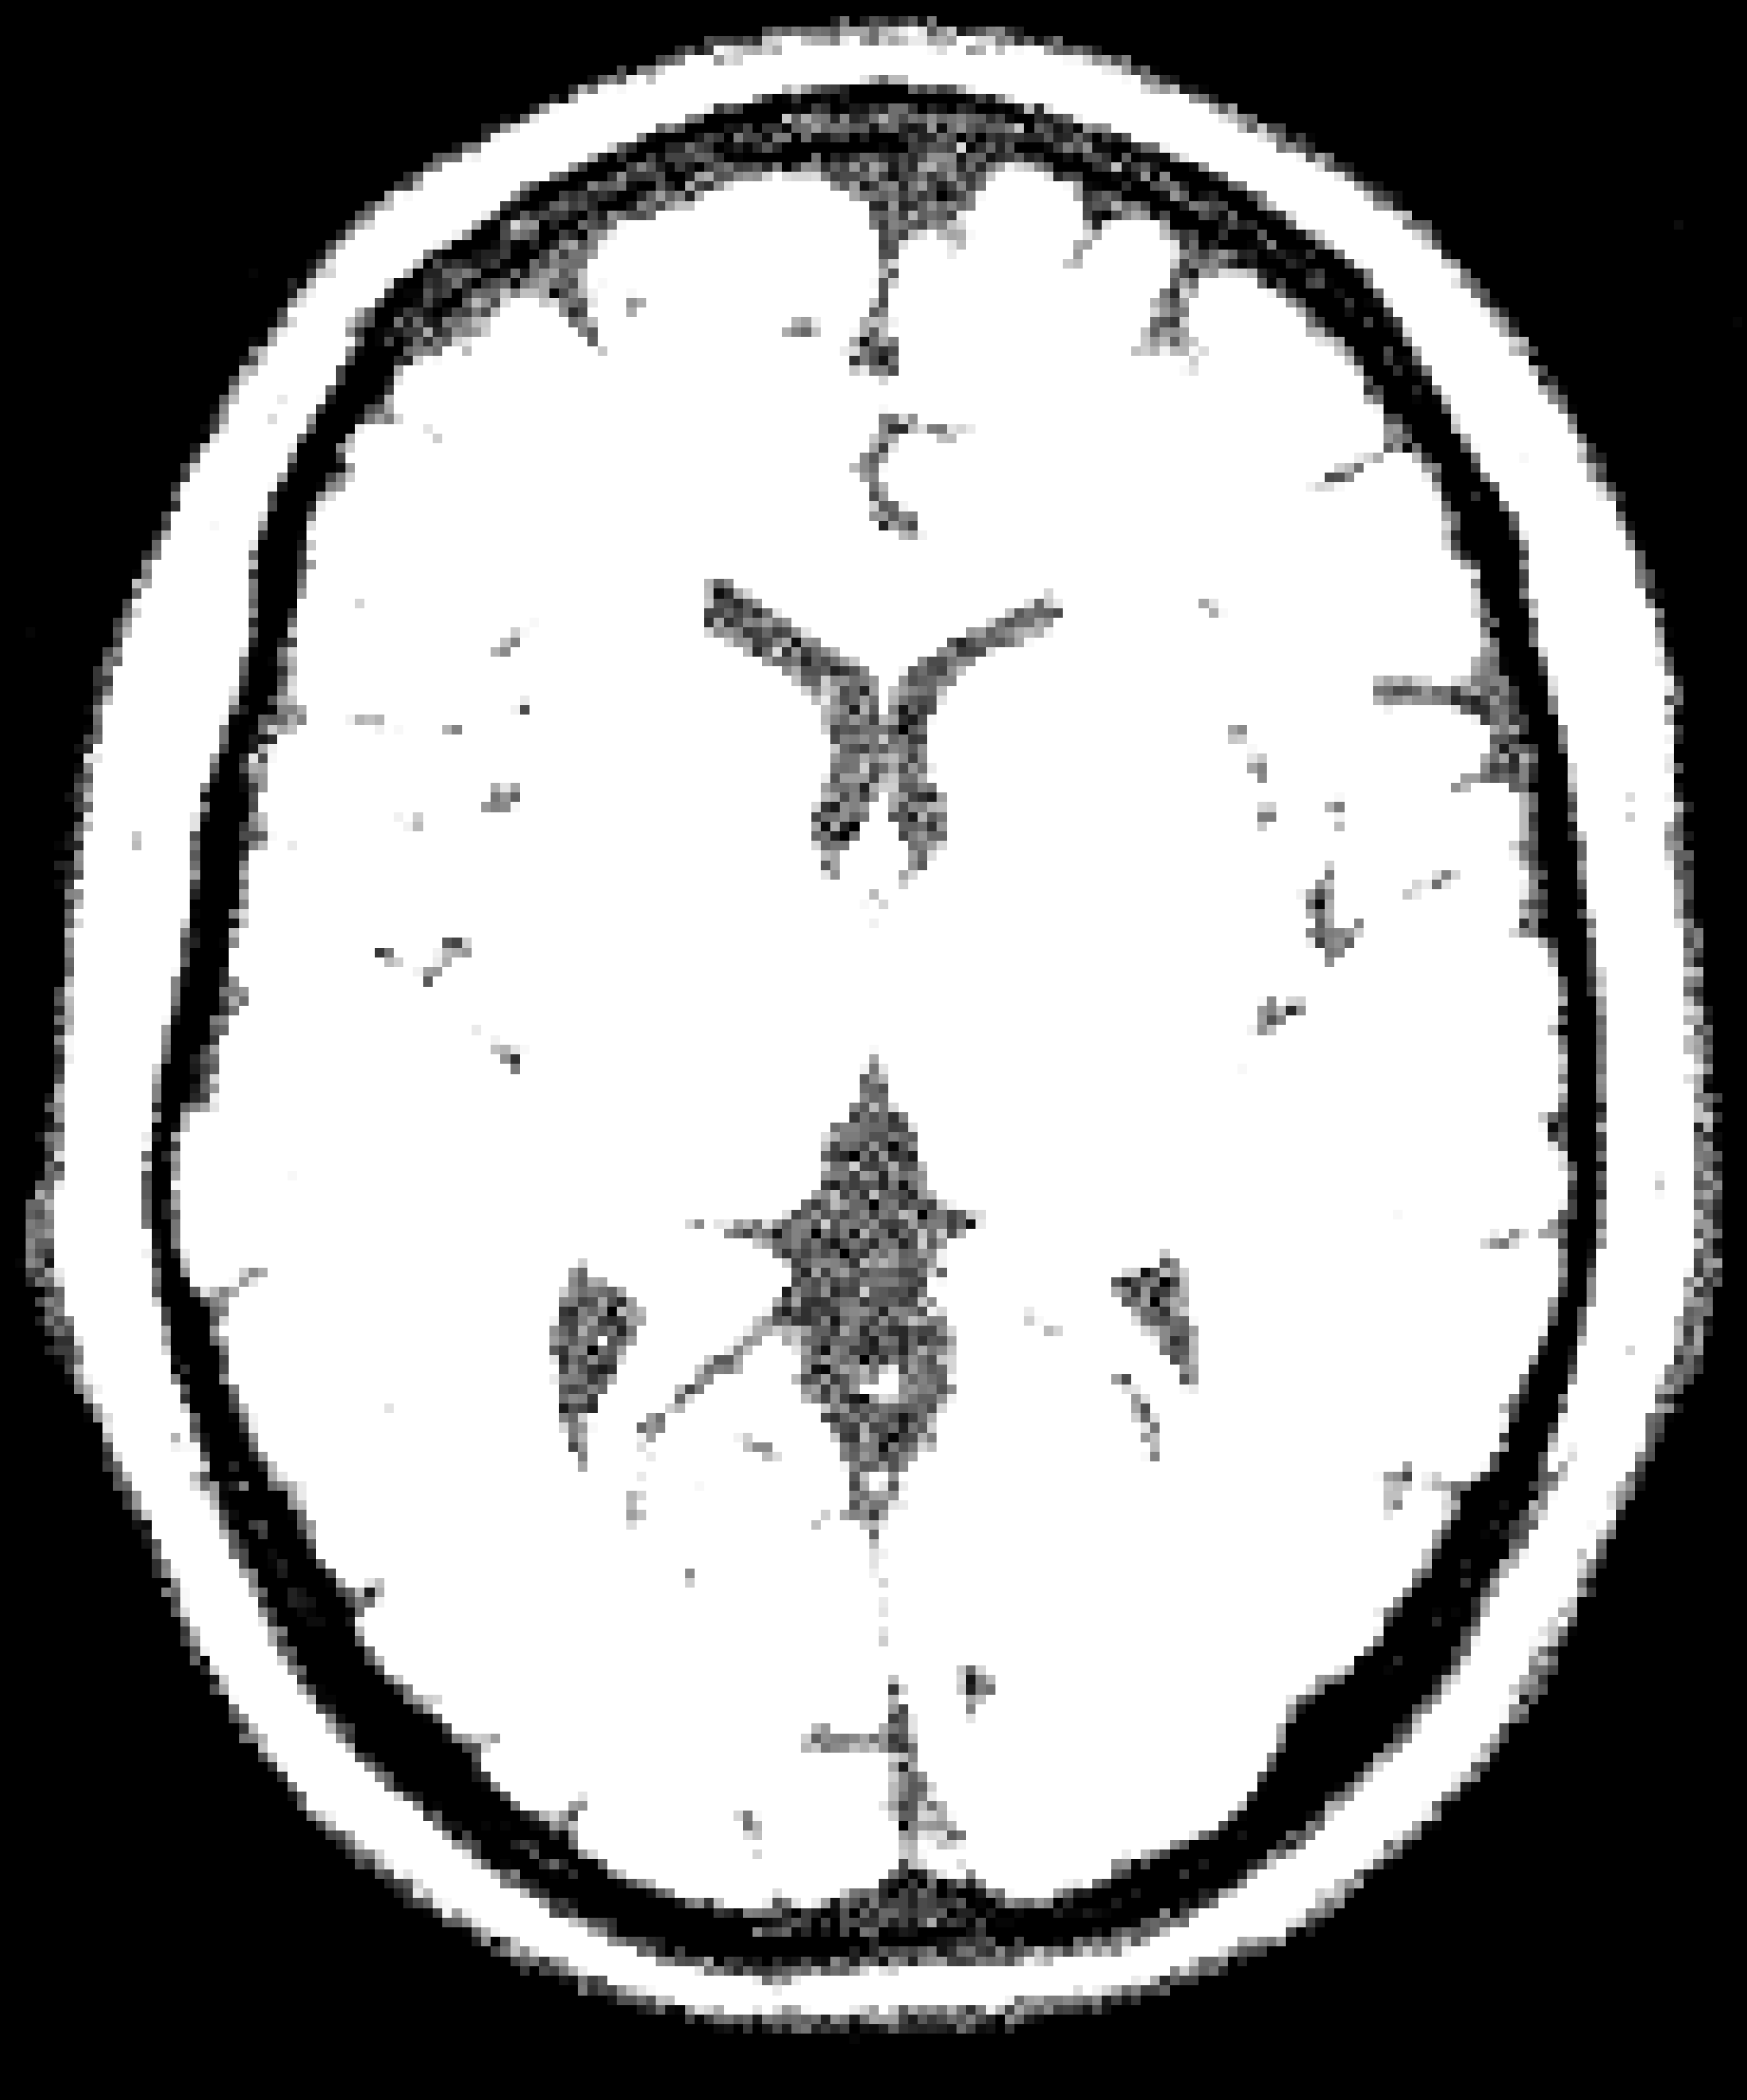
\includegraphics[width=\textwidth]{Figuras/ImageA_25_62.png}
            \caption{Líquido \\ 
            $~$} 
         \end{subfigure}
         \begin{subfigure}[h]{0.24\linewidth}
            \centering
            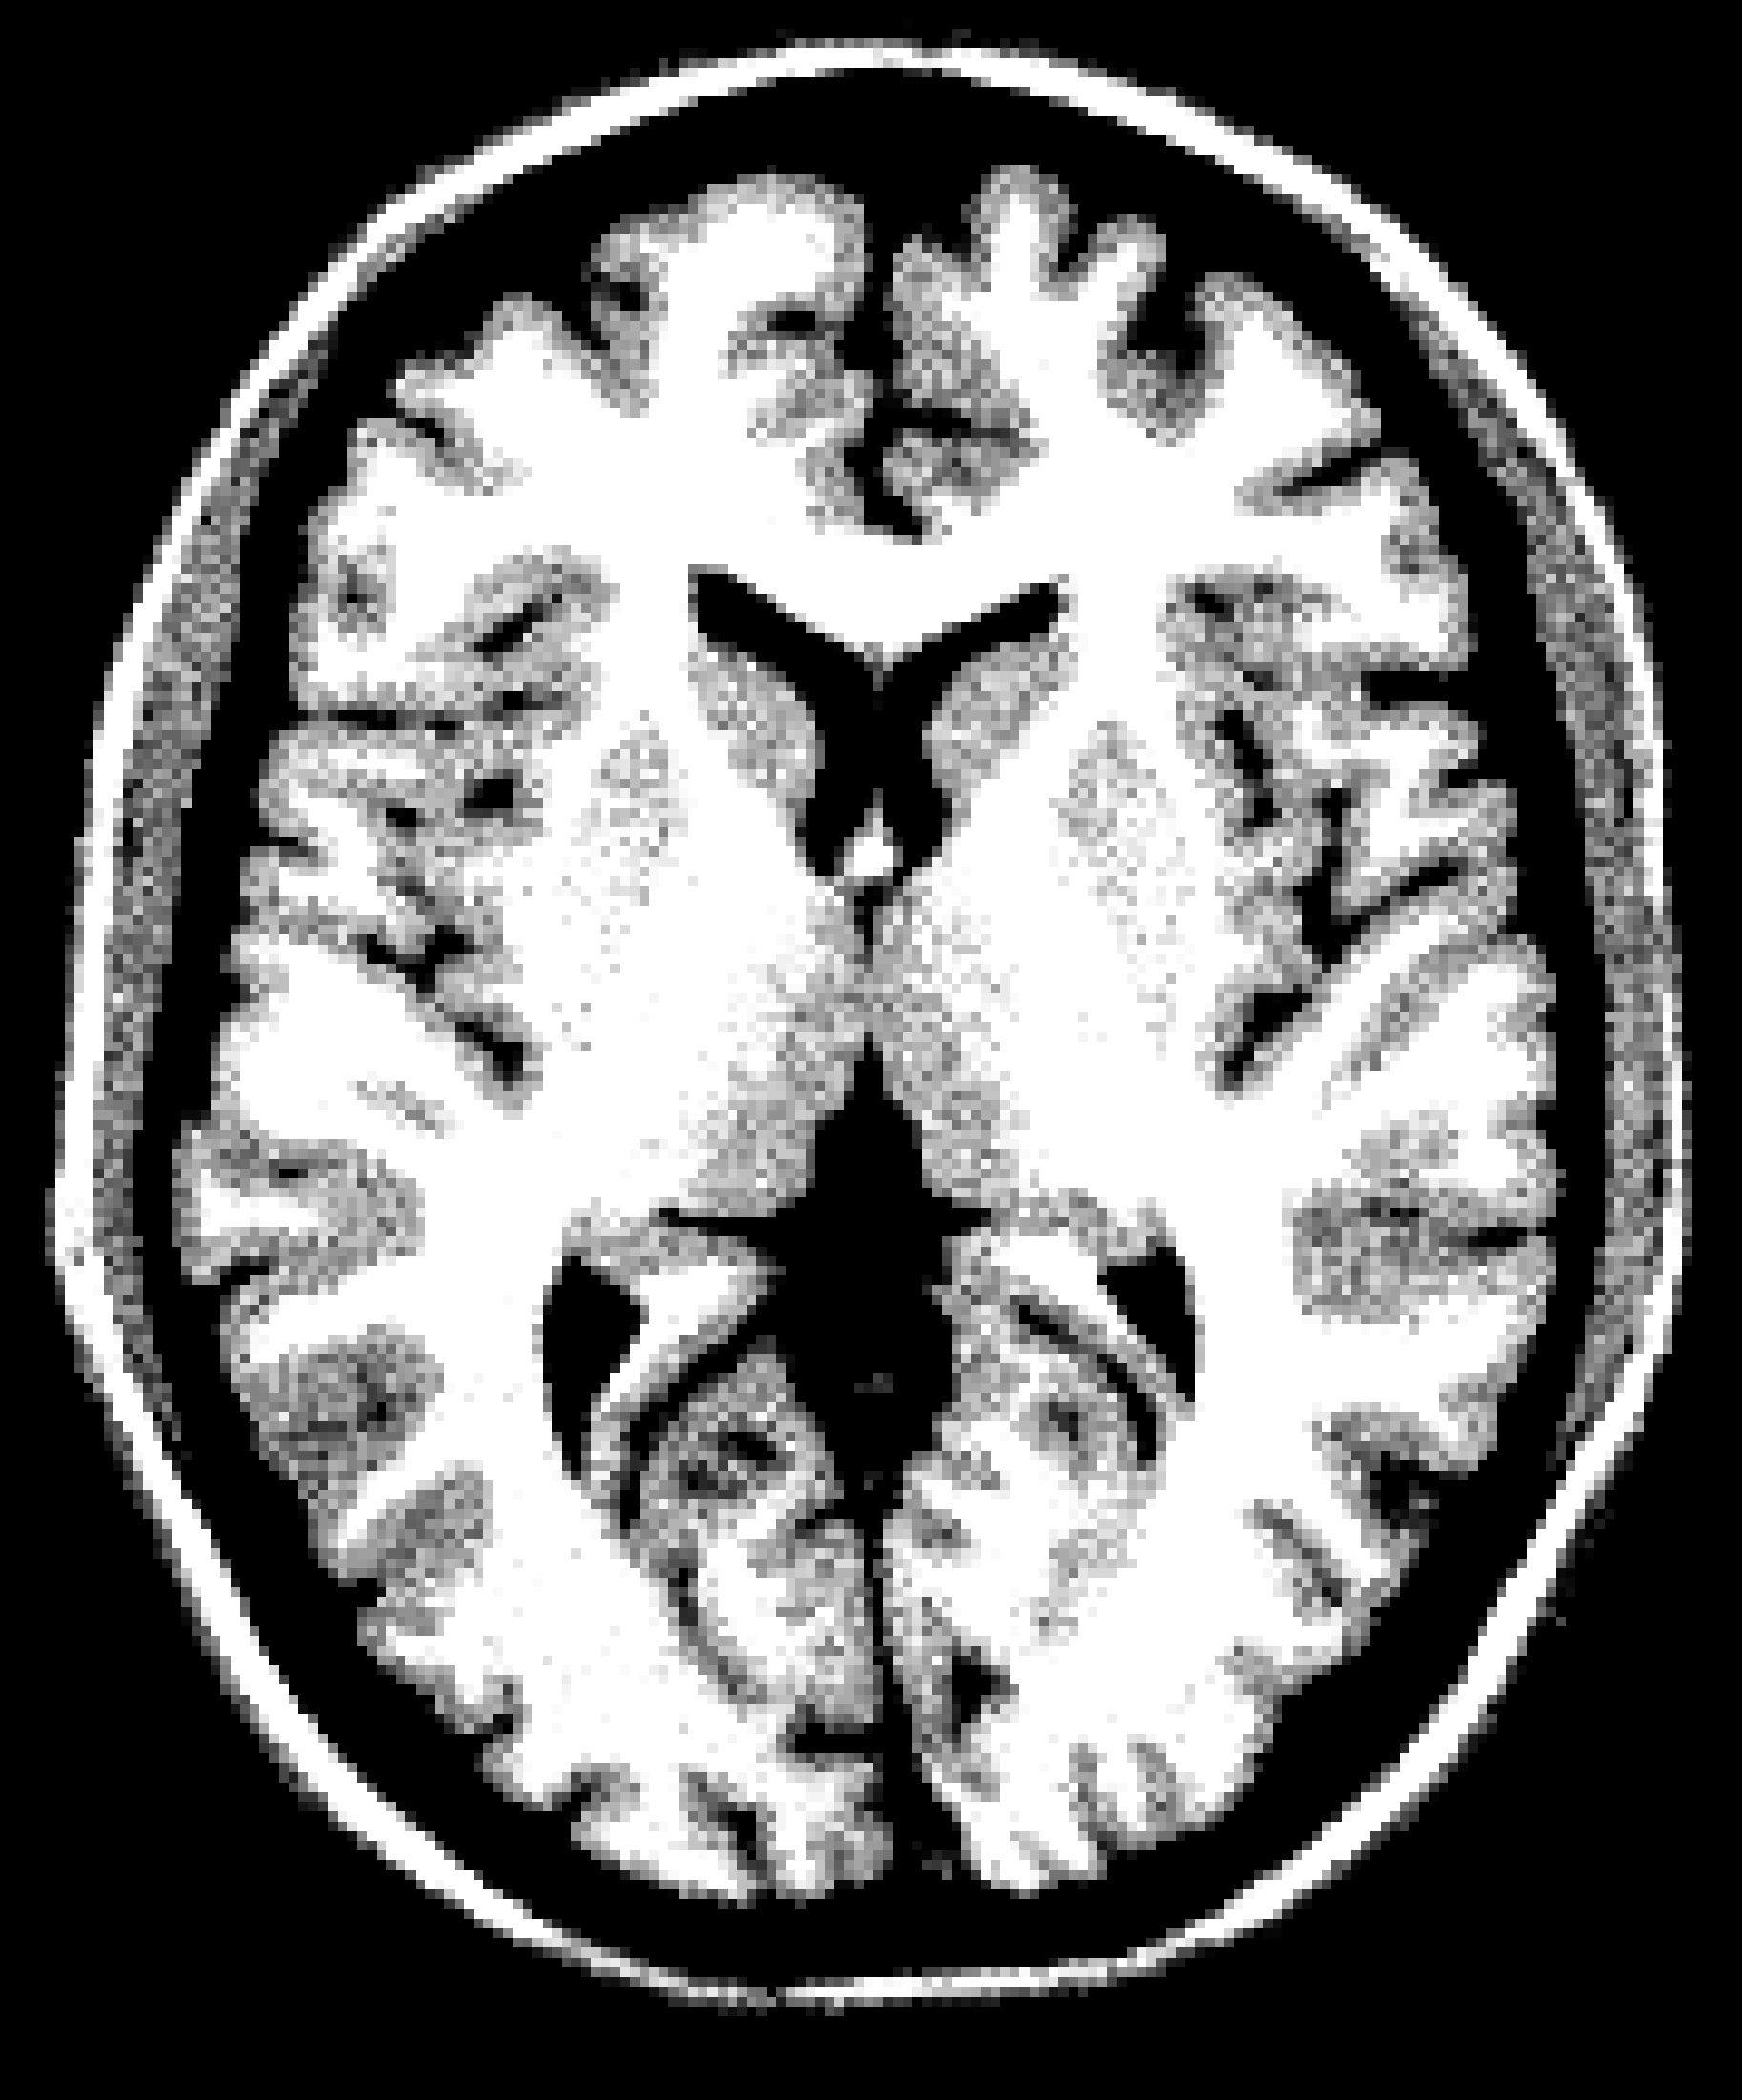
\includegraphics[width=\textwidth]{Figuras/ImageA_62_113.png}
            \caption{Materia gris} 
         \end{subfigure}
         \begin{subfigure}[h]{0.24\linewidth}
            \centering
            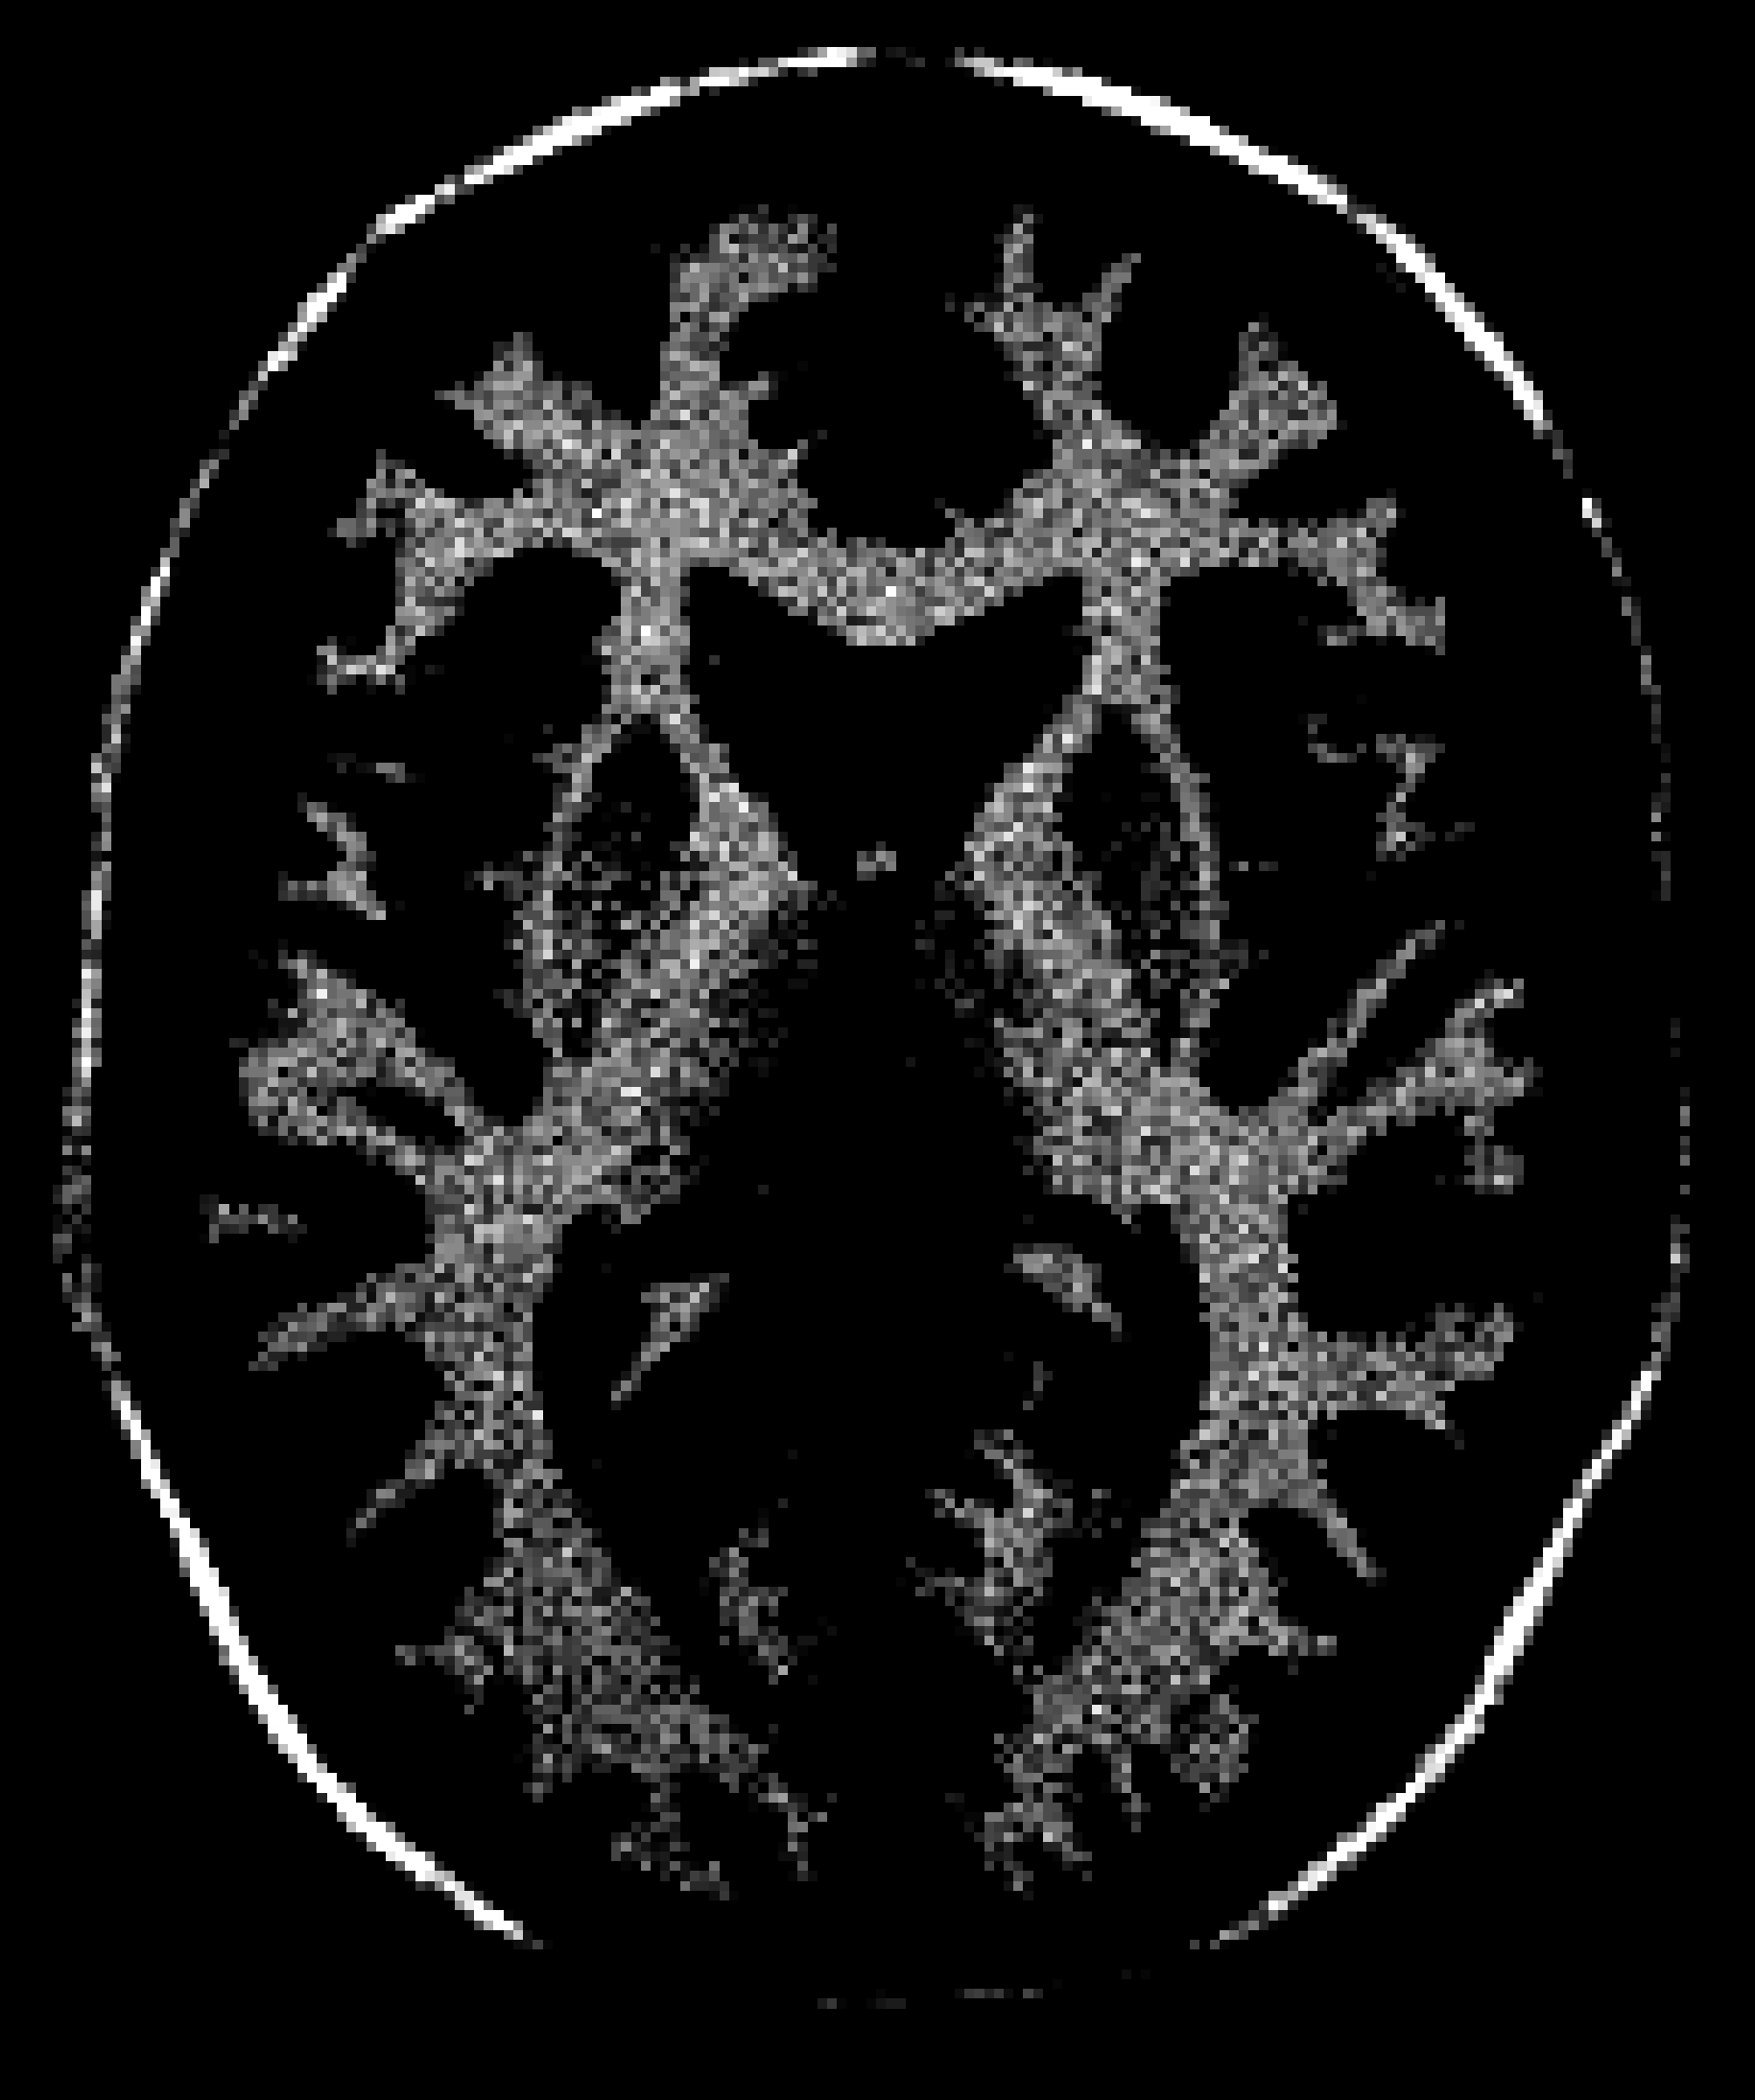
\includegraphics[width=\textwidth]{Figuras/ImageA_113_150.png}
            \caption{Materia blanca} 
         \end{subfigure}
    \caption{Transformación semilinear aplicada a distintas regiones de la imagen original.%(a) Fondo (b) Líquido (c) Materia gris (d) Materia blanca.
    }
    \label{fig:Semilineartrans_region}
\end{figure}

Por otro lado, se ecualizó la imagen A como se muestra en la Fig. \ref{fig:EQ}. La ecualización corresponde a una trasnformación de la forma
\begin{equation}
    T(r) ) (I_{max} - I_{min}) \sum_{i=0}^{r} P(i)
\end{equation}
donde $P(i)$ es la distribución de probabilidad de que un pixel tenga intensidad $i$. En particular, se toma esta distribución normalizando el histograma de intensidades de la imagen original. Se observa que se expande el rango dinámico, mejorando el contraste de la imagen sin acumulación de intensidades como sucedía en la transformación semilinear.

\begin{figure}[h]
    \centering
        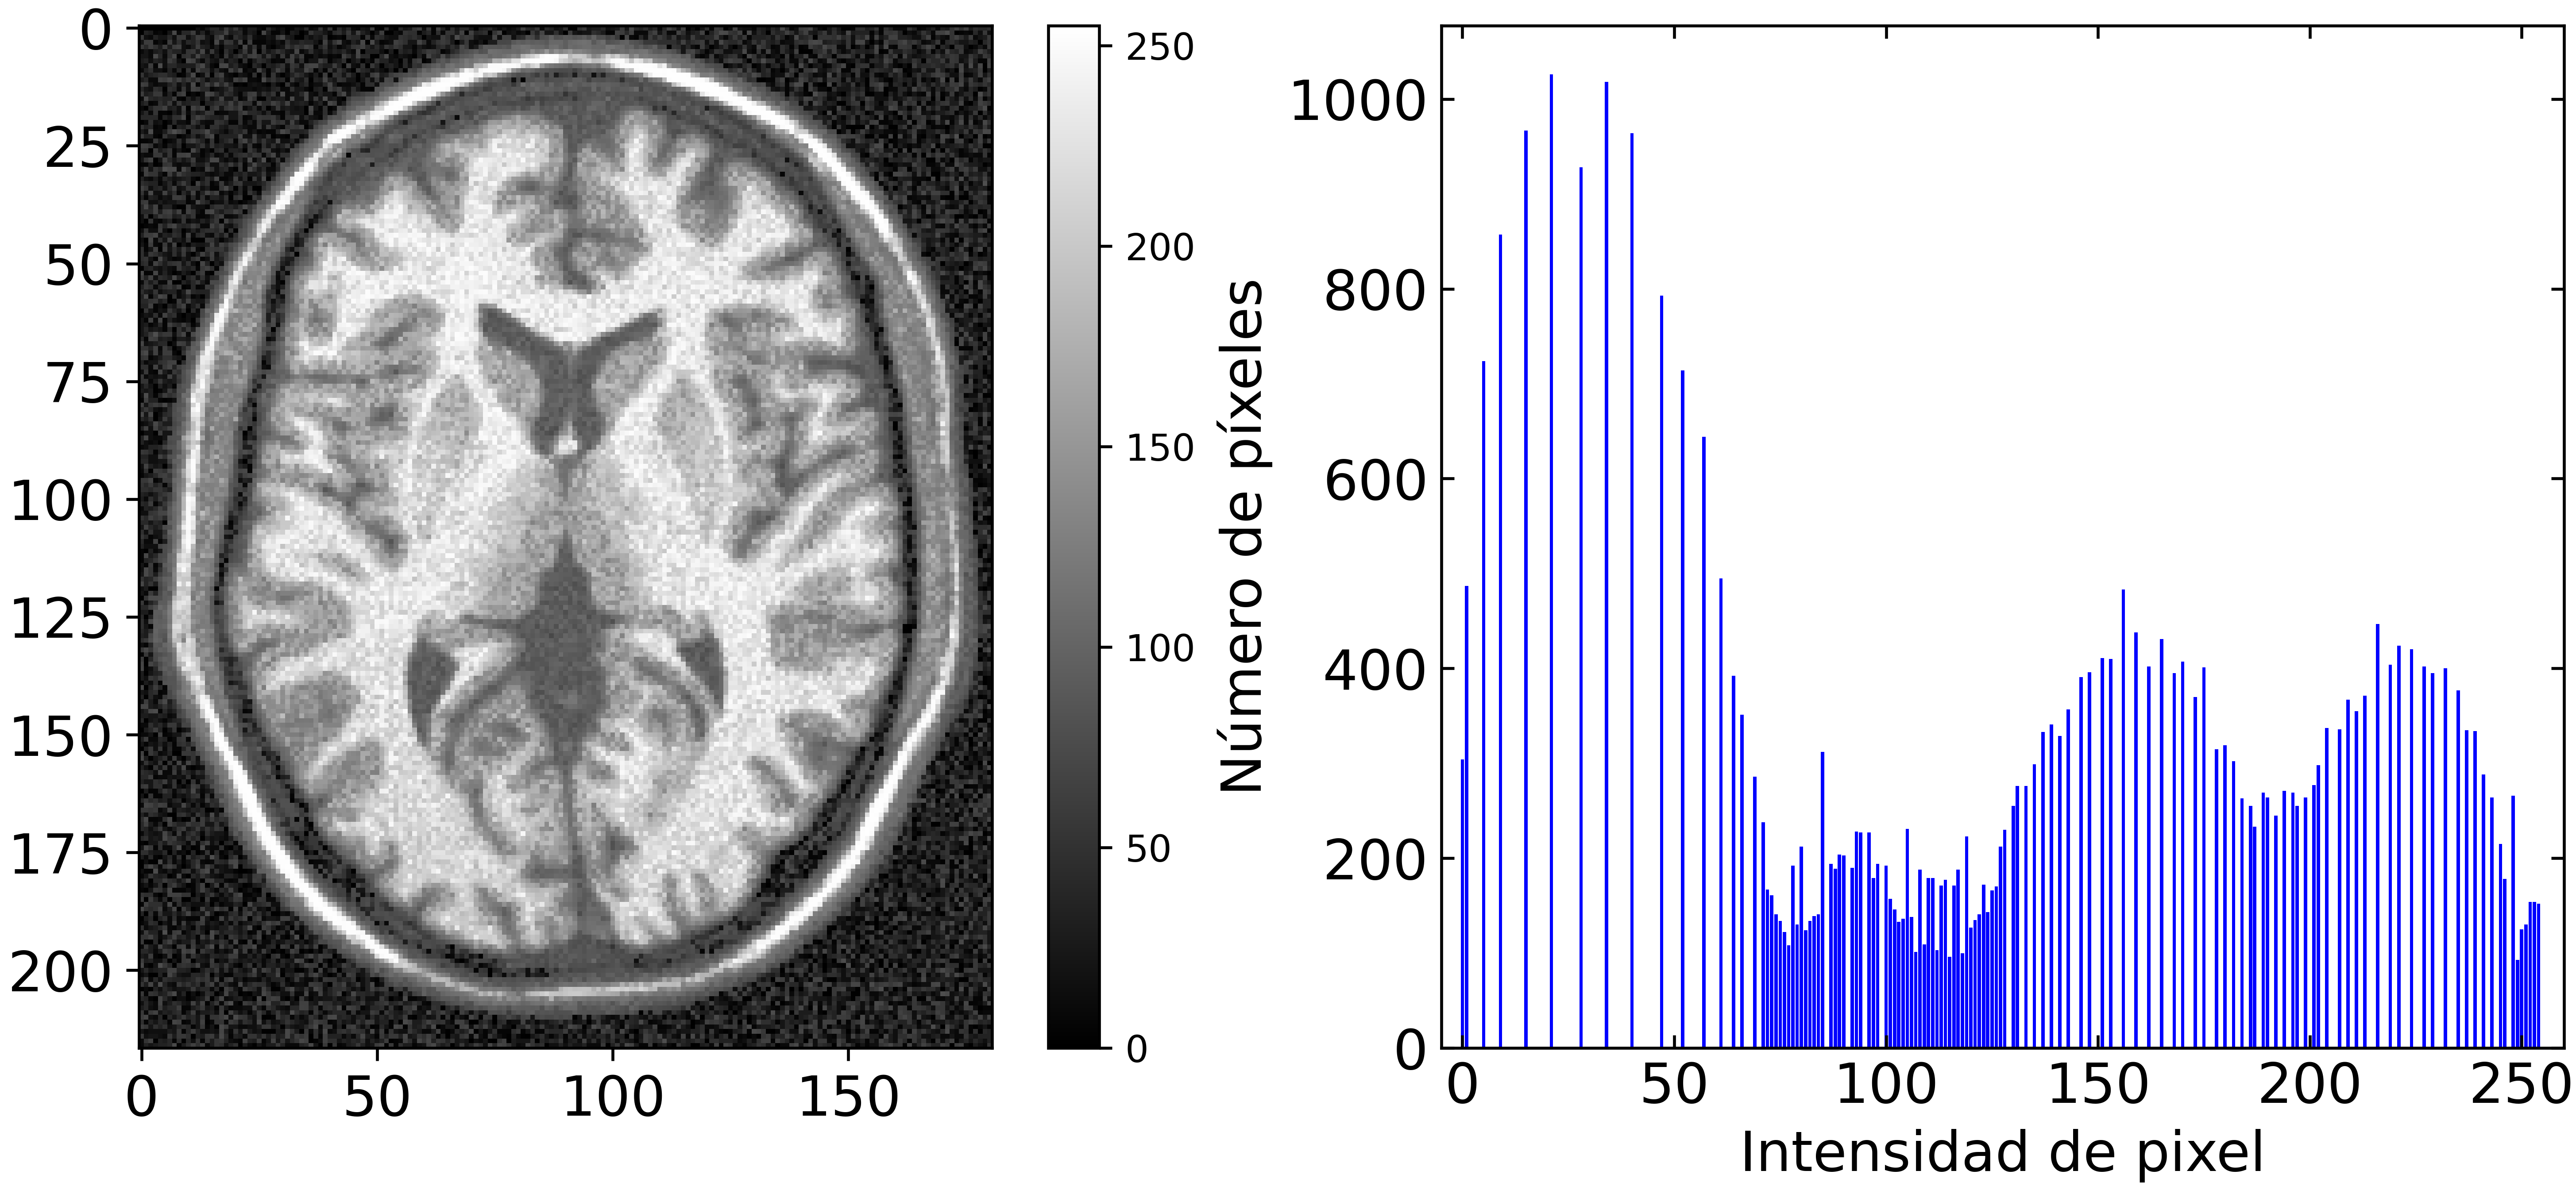
\includegraphics[width=\linewidth]{Figuras/ImageA_EQ_hist.png}
    \caption{ImagenA ecualizada junto con su histograma de intensidades.} 
    \label{fig:EQ}
\end{figure}

Se pueden realizar otras transformaciones de contraste, como la binarización de la imagen, que consiste en transformar la imagen según 
\begin{equation}
    T(r) = 
    \begin{cases}
    0 & \text{si } r \geq 128 \\
    255 & \text{si } r < 128
    \end{cases}
\end{equation}
o una transformación según una ley de potencias de la forma
\begin{equation}
    T(r) = I_{max} \biggr( \frac{r}{r_{max}}\biggr)^\gamma
\end{equation}
donde se tomó $I_{max} = 255$ y distintos valores de $\gamma$.

En la Fig. \ref{fig:binarytrans} se muestra la imagen binarizada de la imagen A original.Esta transformación muestra en negro los valores de la imagen por encima de un cierto umbral, en este caso 128, y en blanco el resto. Esto sirve para resaltar estructuras por encima de dicho umbral eliminando el resto de información de la imagen. 

En la Fig. \ref{fig:Exptrans} se muestra la transformación $\gamma$ aplicada a la imagenA original. En este caso se ve que valores de $\gamma < 1$ generan una imagen más brillante y valores de $\gamma > 1 $ más oscura.

\begin{figure}[h]
    \centering
        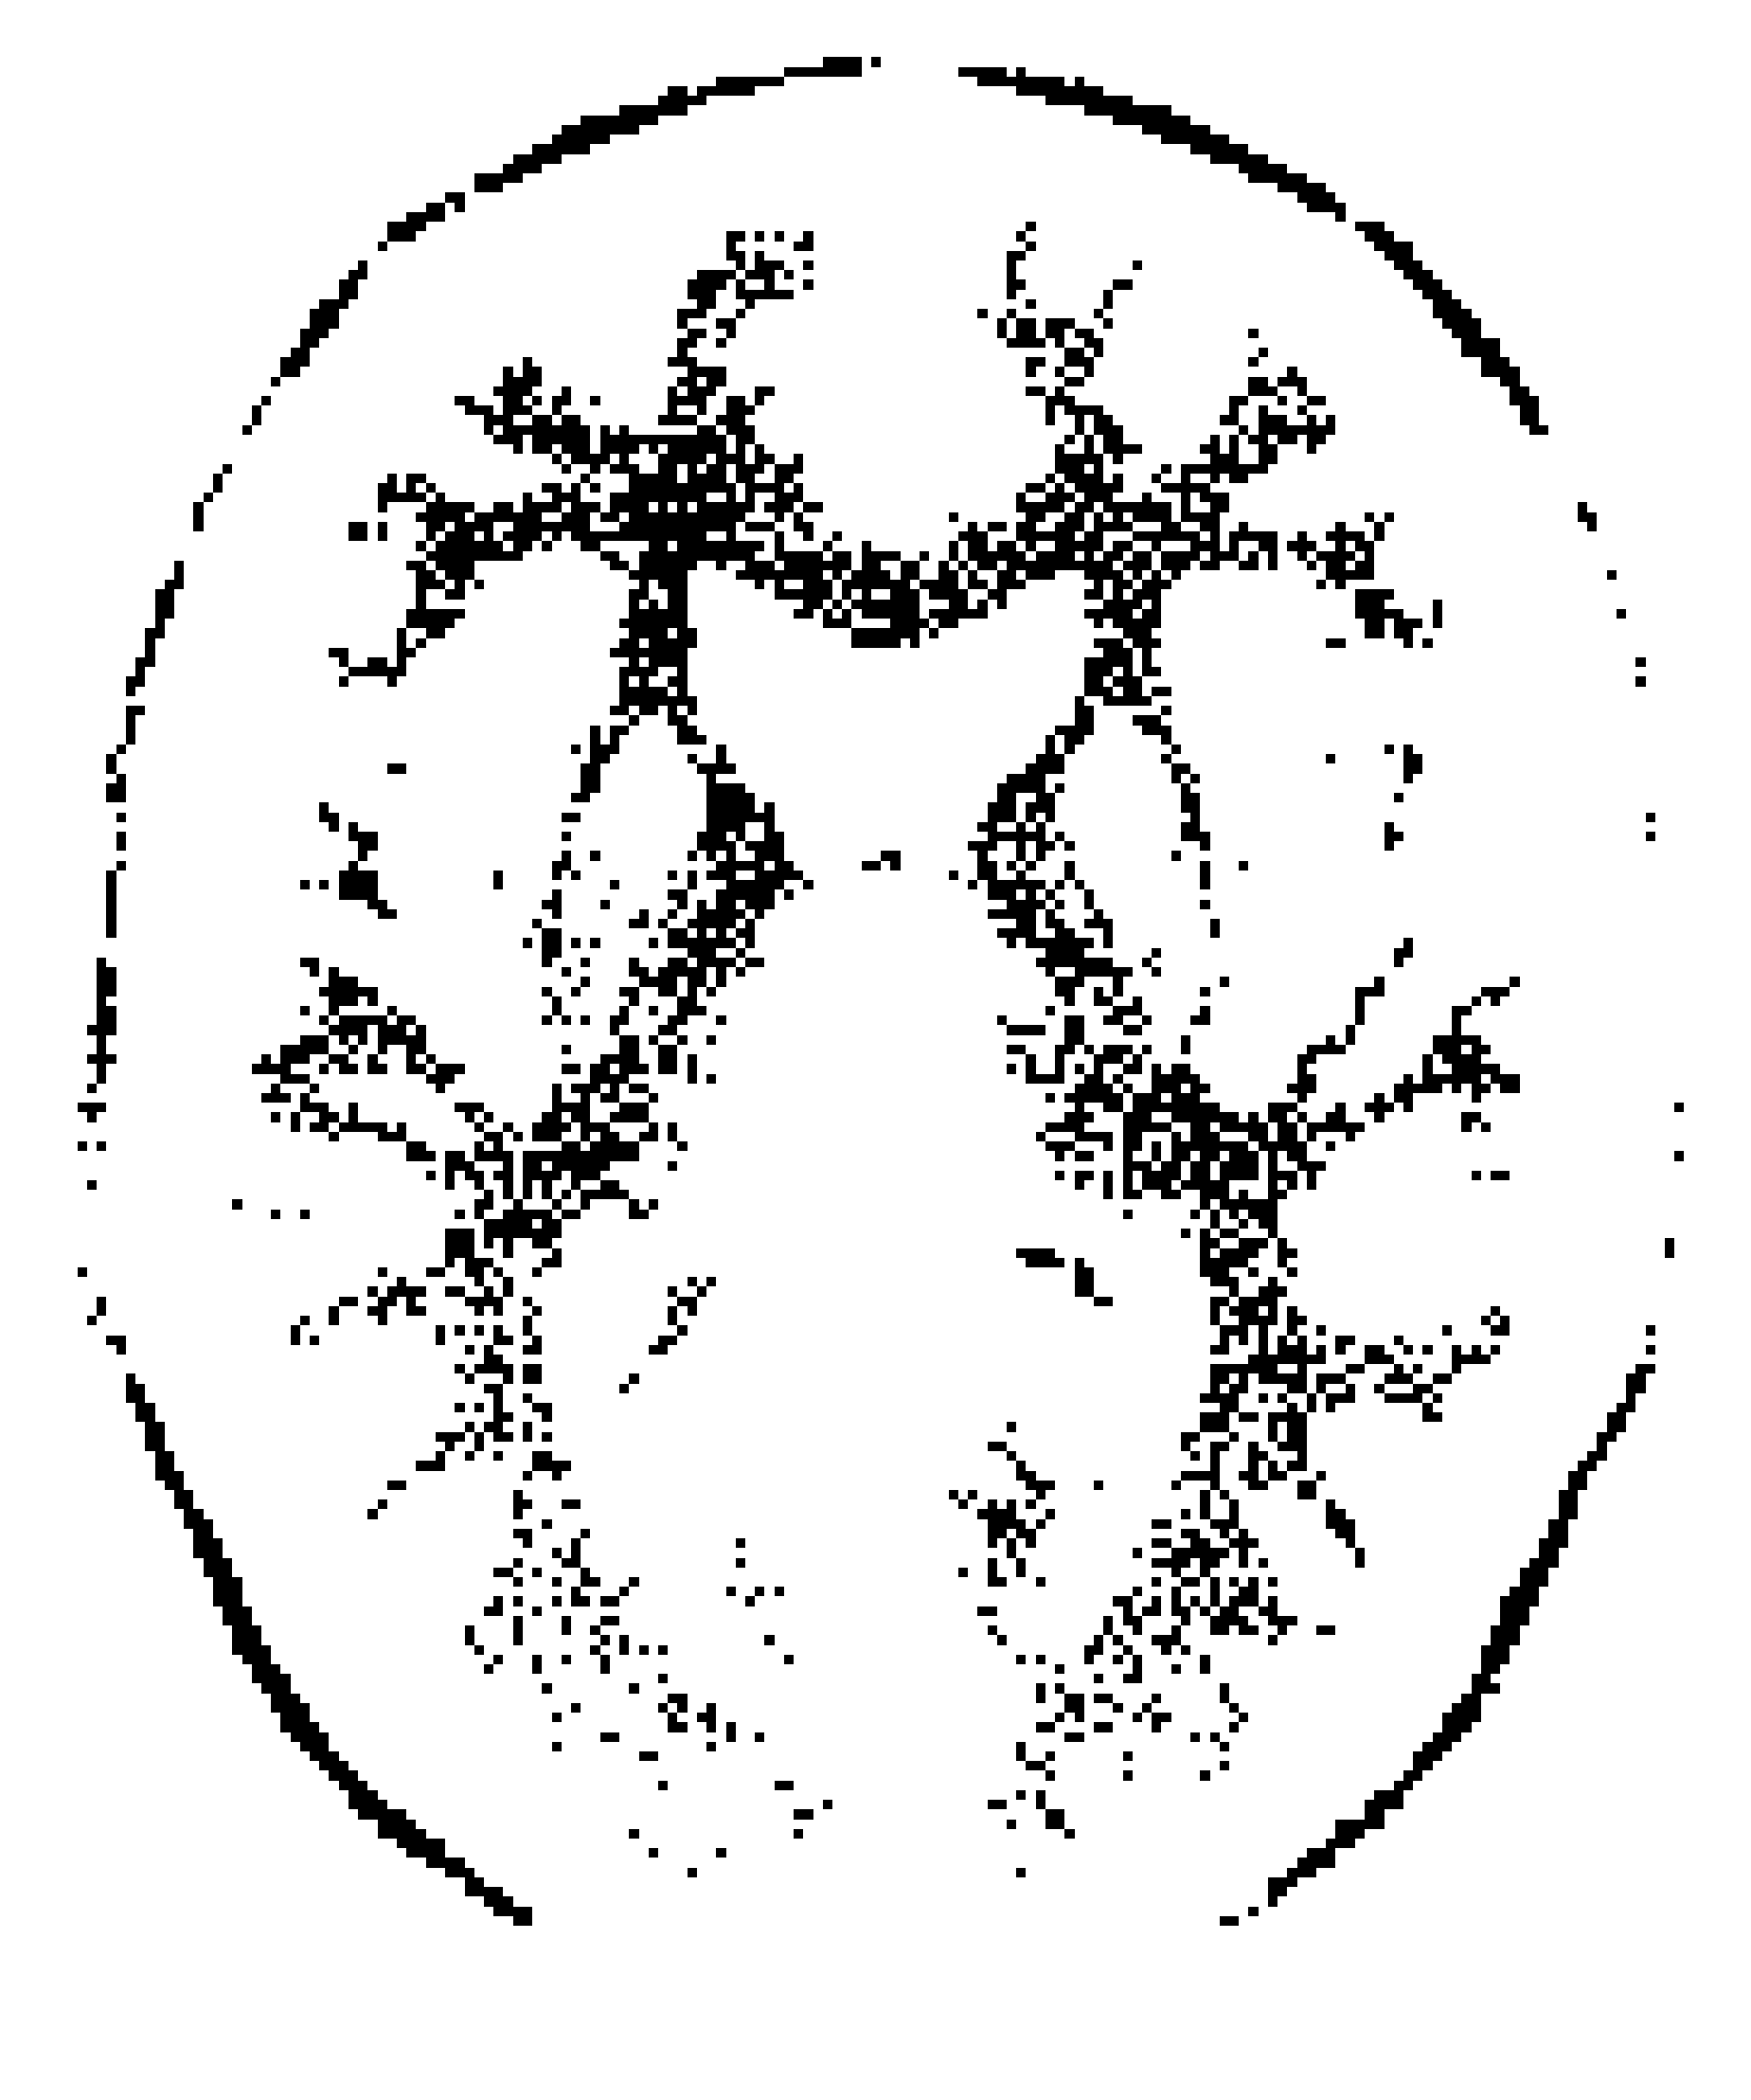
\includegraphics[width=0.4\linewidth]{Figuras/ImageA_binary.png}
    \caption{Transformación binaria aplicada a la imagenA original.}
    \label{fig:binarytrans}
\end{figure}

\begin{figure}[H]
    \centering
         \begin{subfigure}[h]{0.32\linewidth}
            \centering
            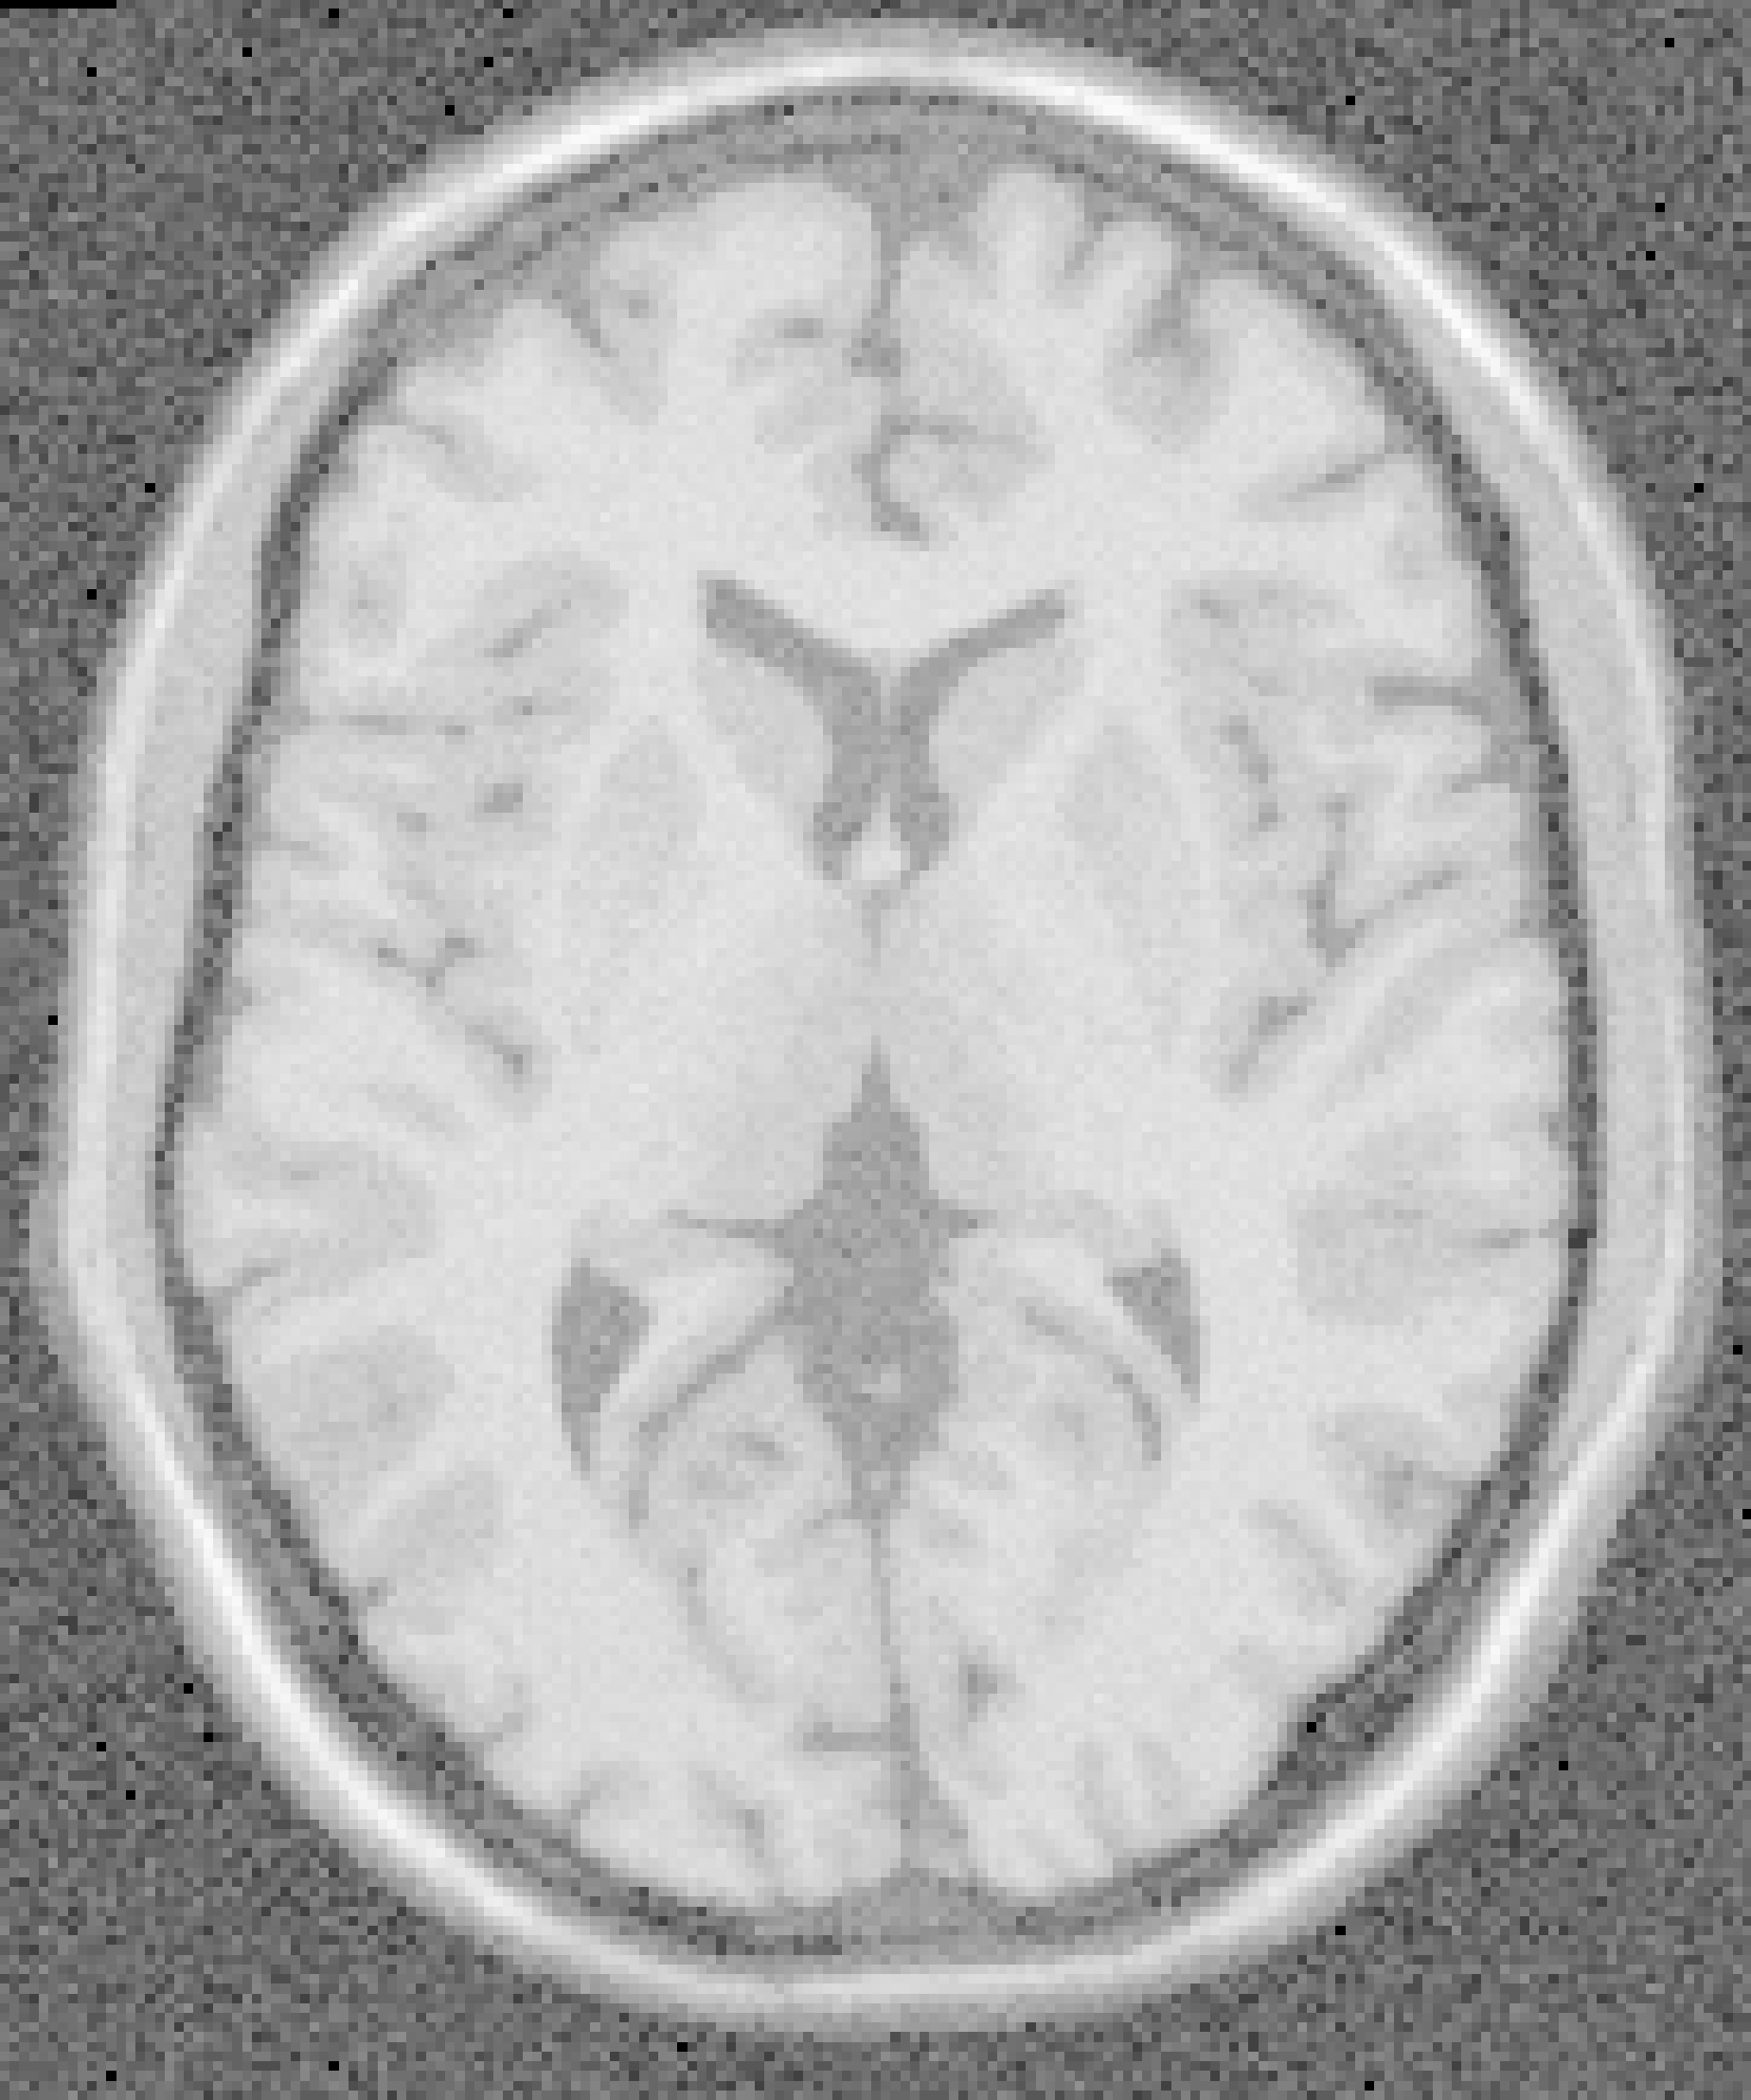
\includegraphics[width=\textwidth]{Figuras/ImageA_exp_gamma=0.25.png}
            \caption{$\gamma = 0.25$} 
         \end{subfigure}
         \begin{subfigure}[h]{0.32\linewidth}
            \centering
            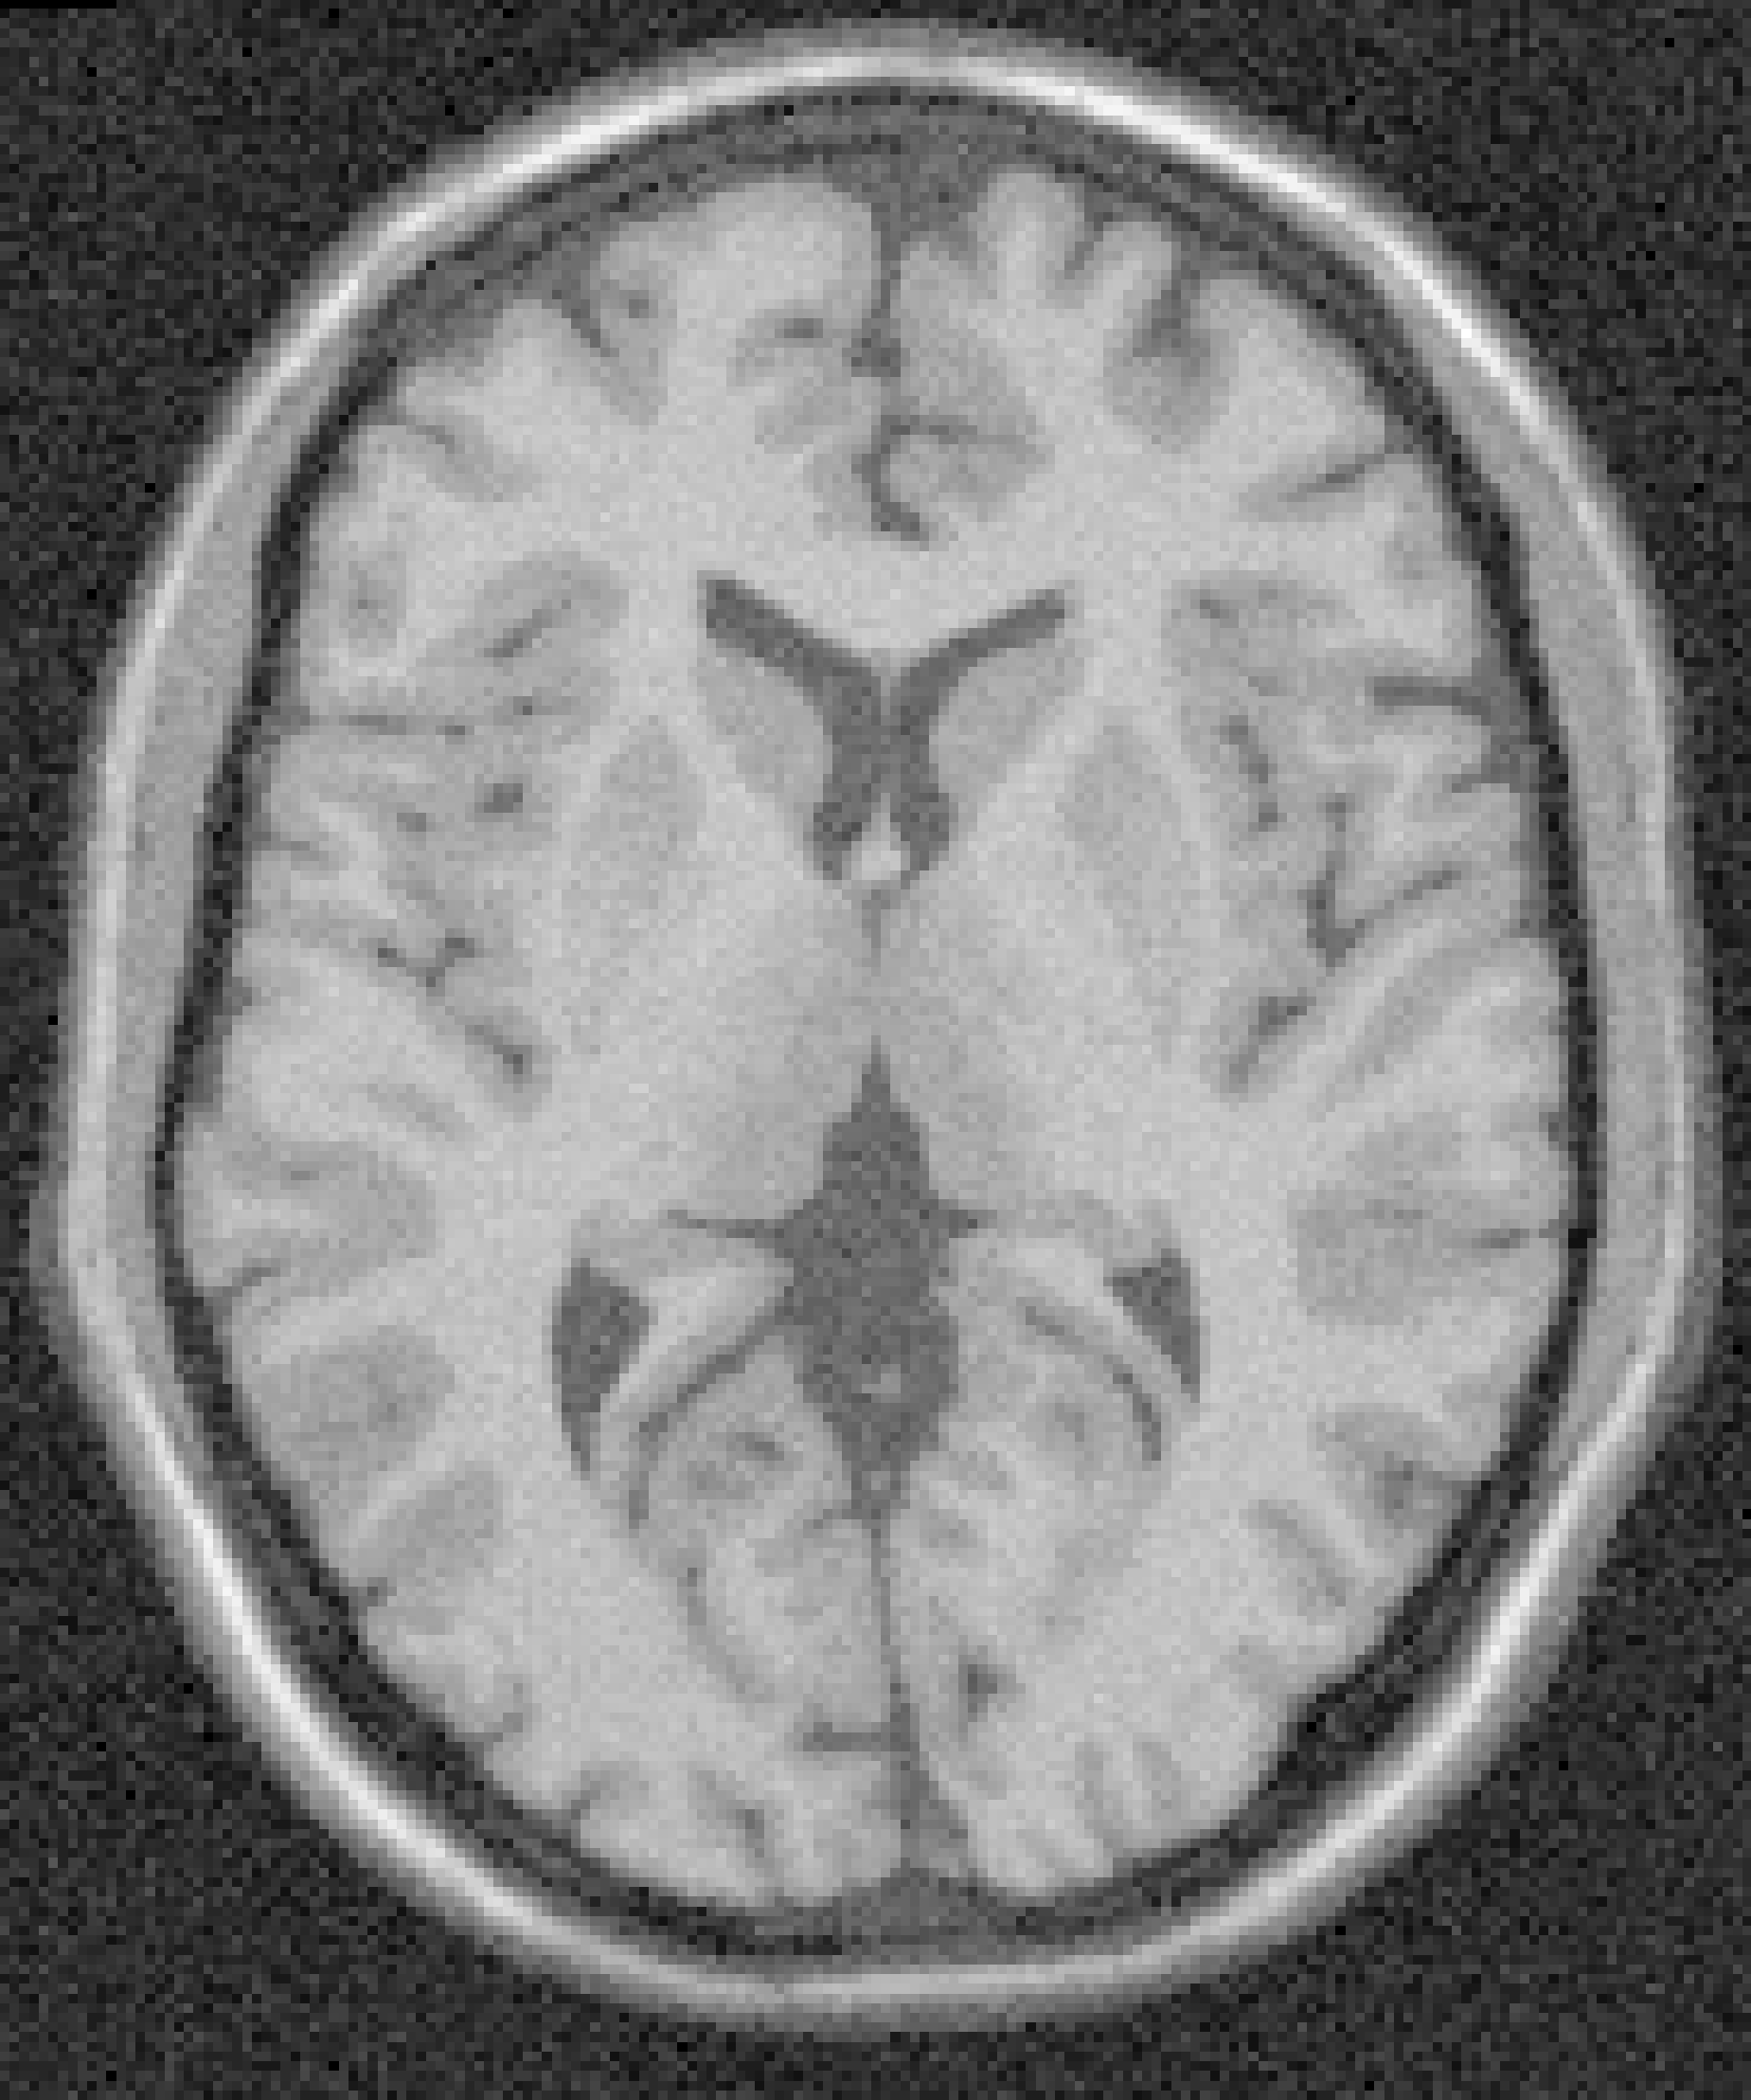
\includegraphics[width=\textwidth]{Figuras/ImageA_exp_gamma=0.5.png}
            \caption{$\gamma = 0.50$} 
         \end{subfigure}
         \begin{subfigure}[h]{0.32\linewidth}
            \centering
            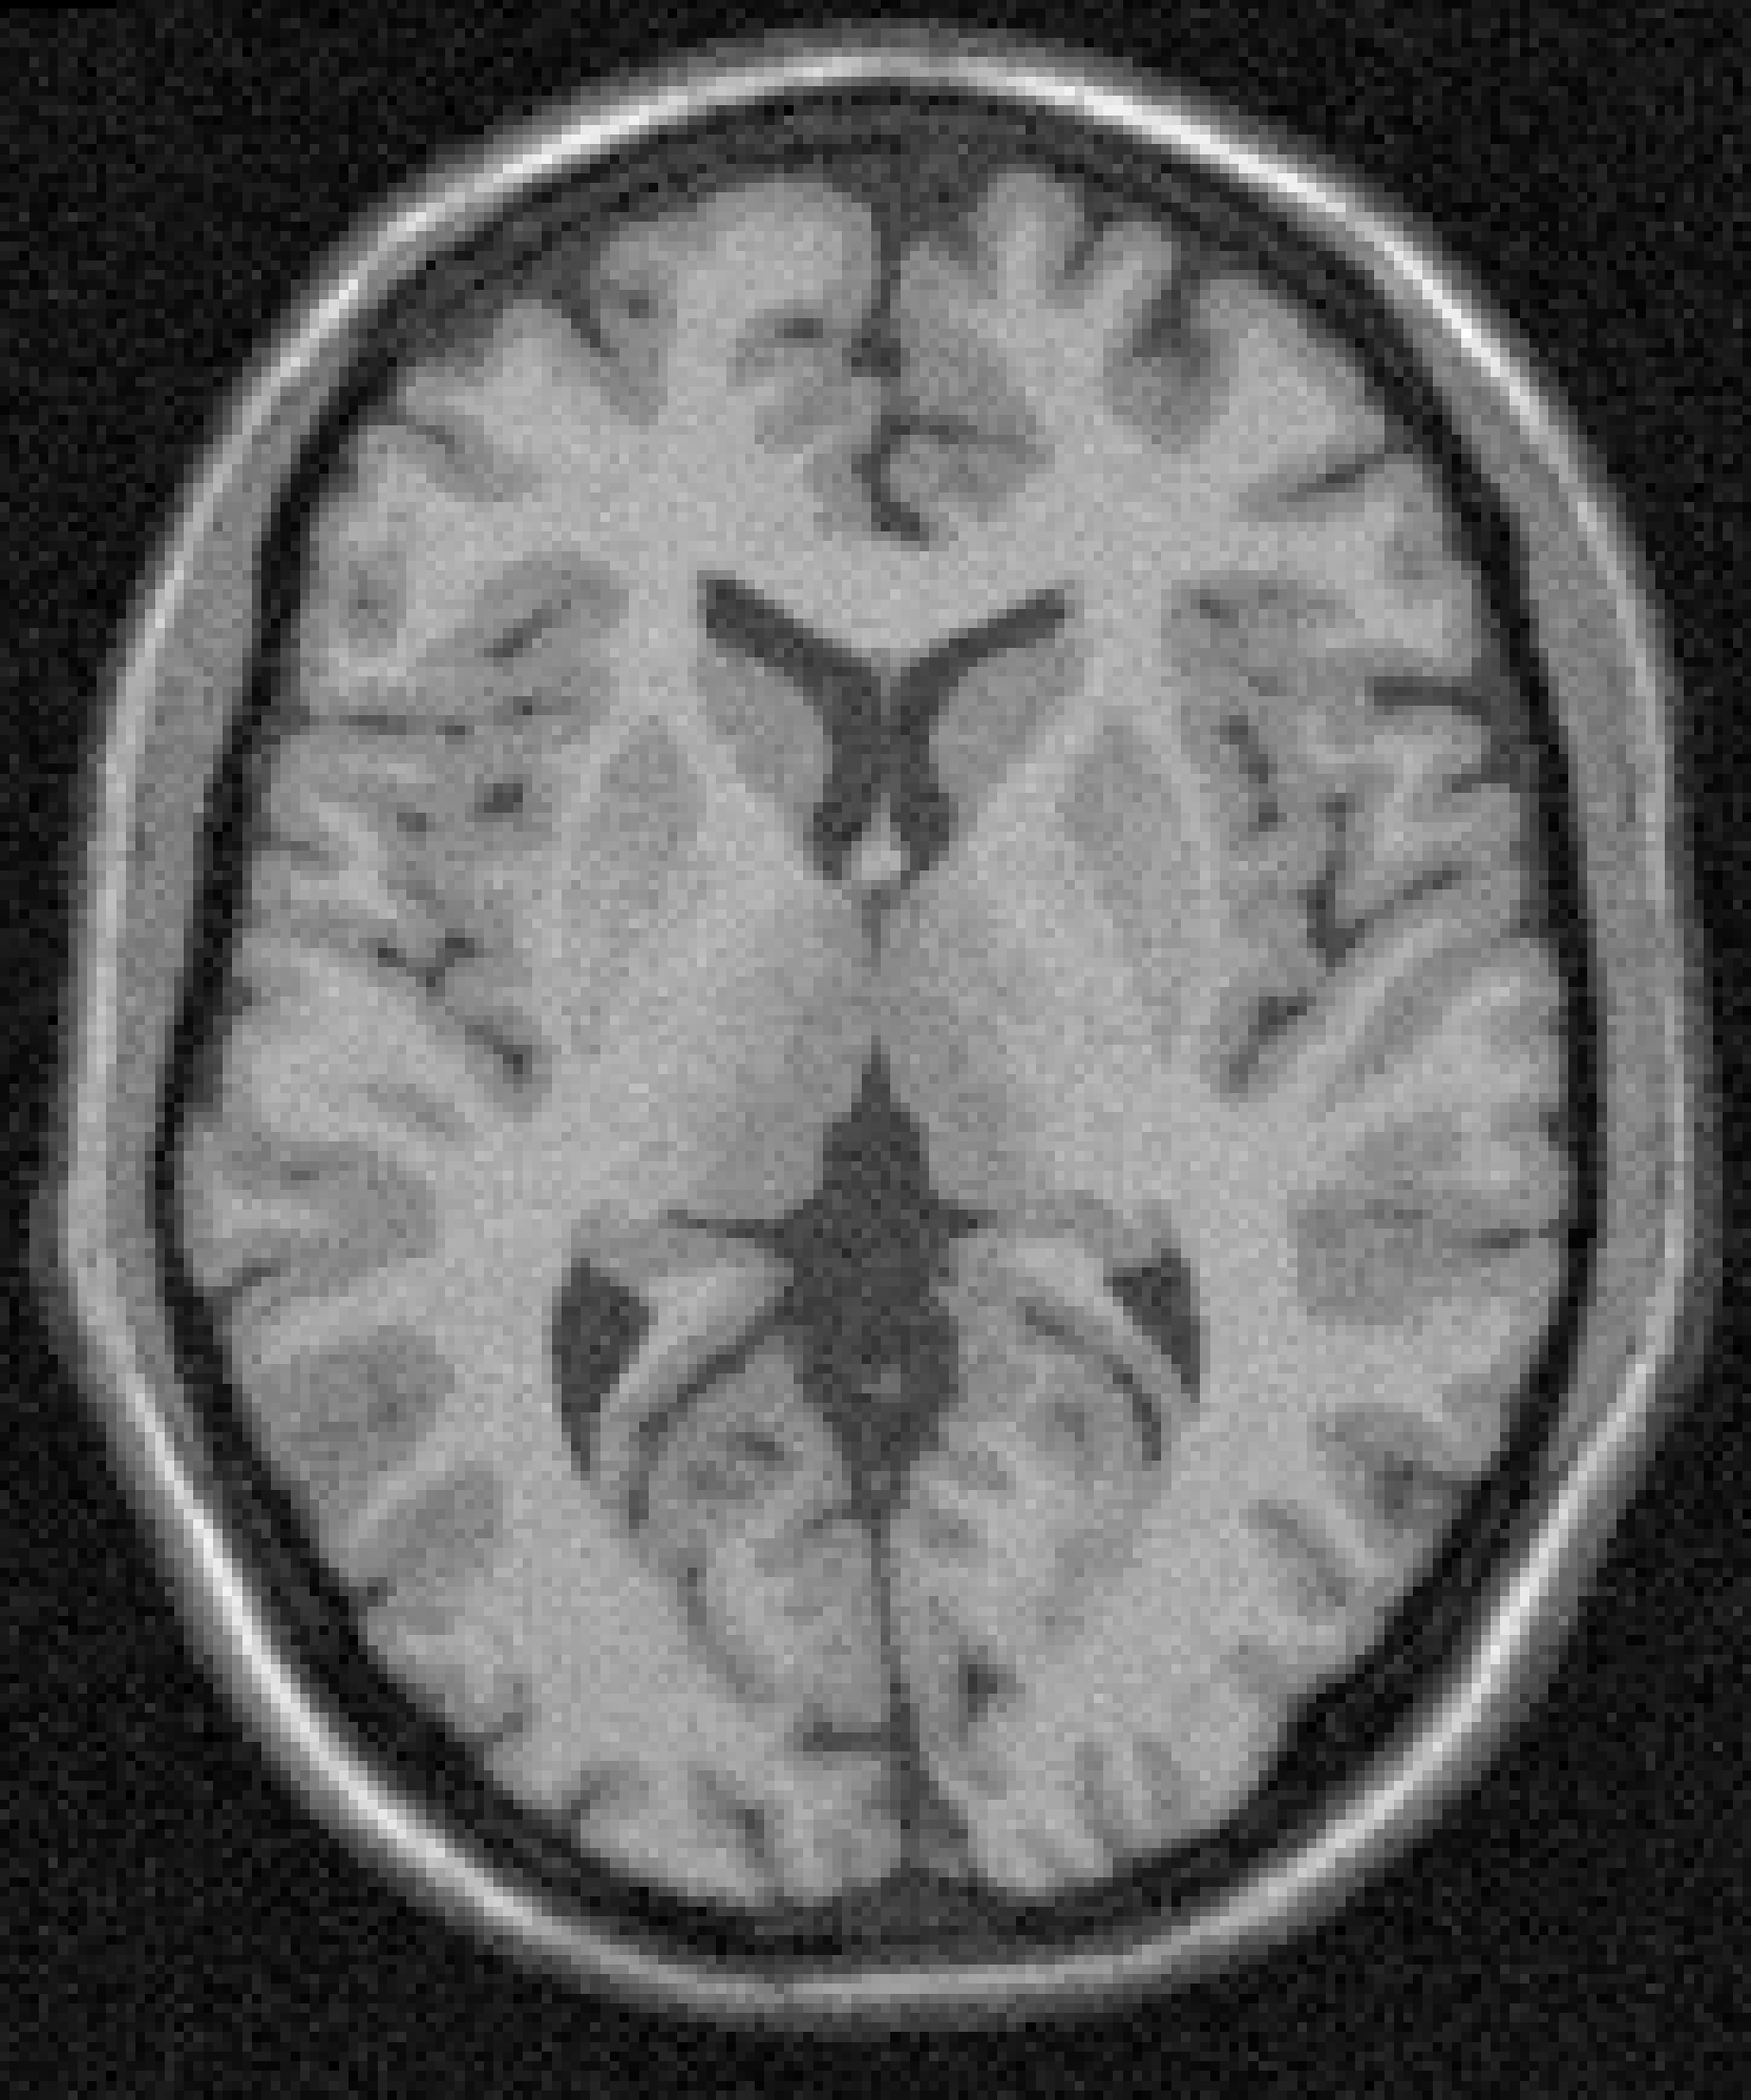
\includegraphics[width=\textwidth]{Figuras/ImageA_exp_gamma=0.75.png}
            \caption{$\gamma = 0.75$} 
         \end{subfigure}
         \begin{subfigure}[h]{0.32\linewidth}
            \centering
            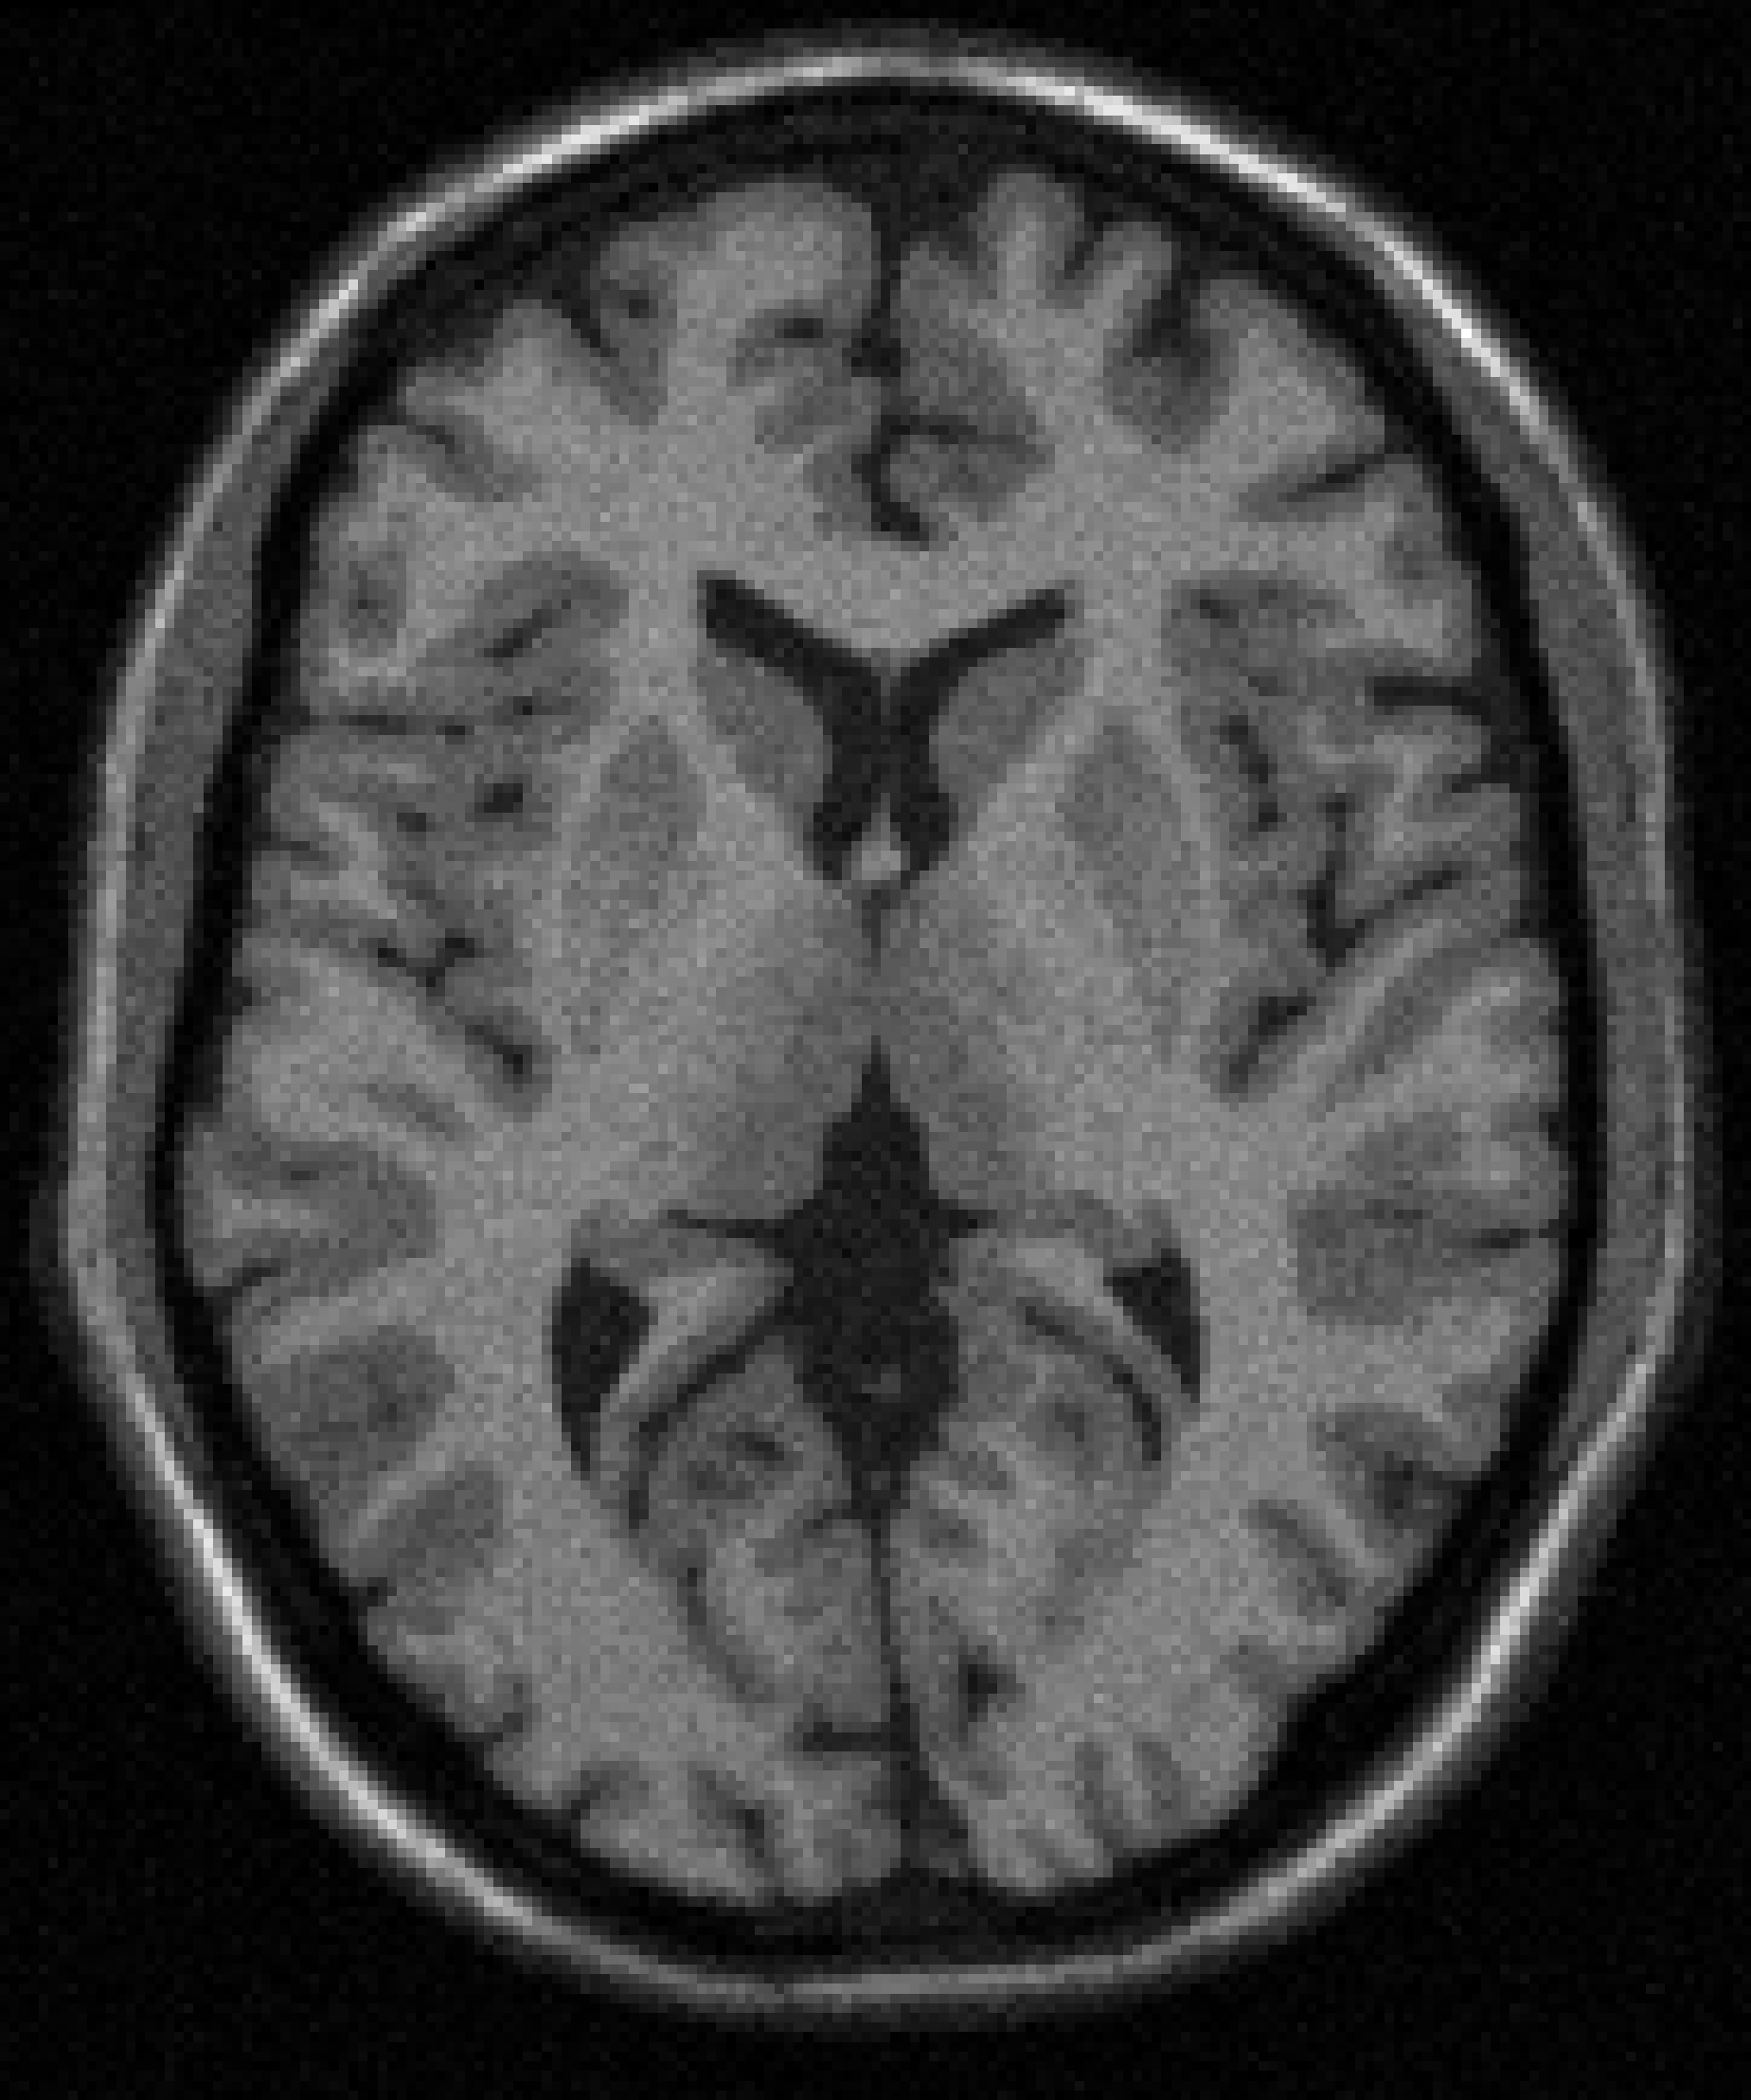
\includegraphics[width=\textwidth]{Figuras/ImageA_exp_gamma=1.25.png}
            \caption{$\gamma = 1.25$} 
         \end{subfigure}
         \begin{subfigure}[h]{0.32\linewidth}
            \centering
            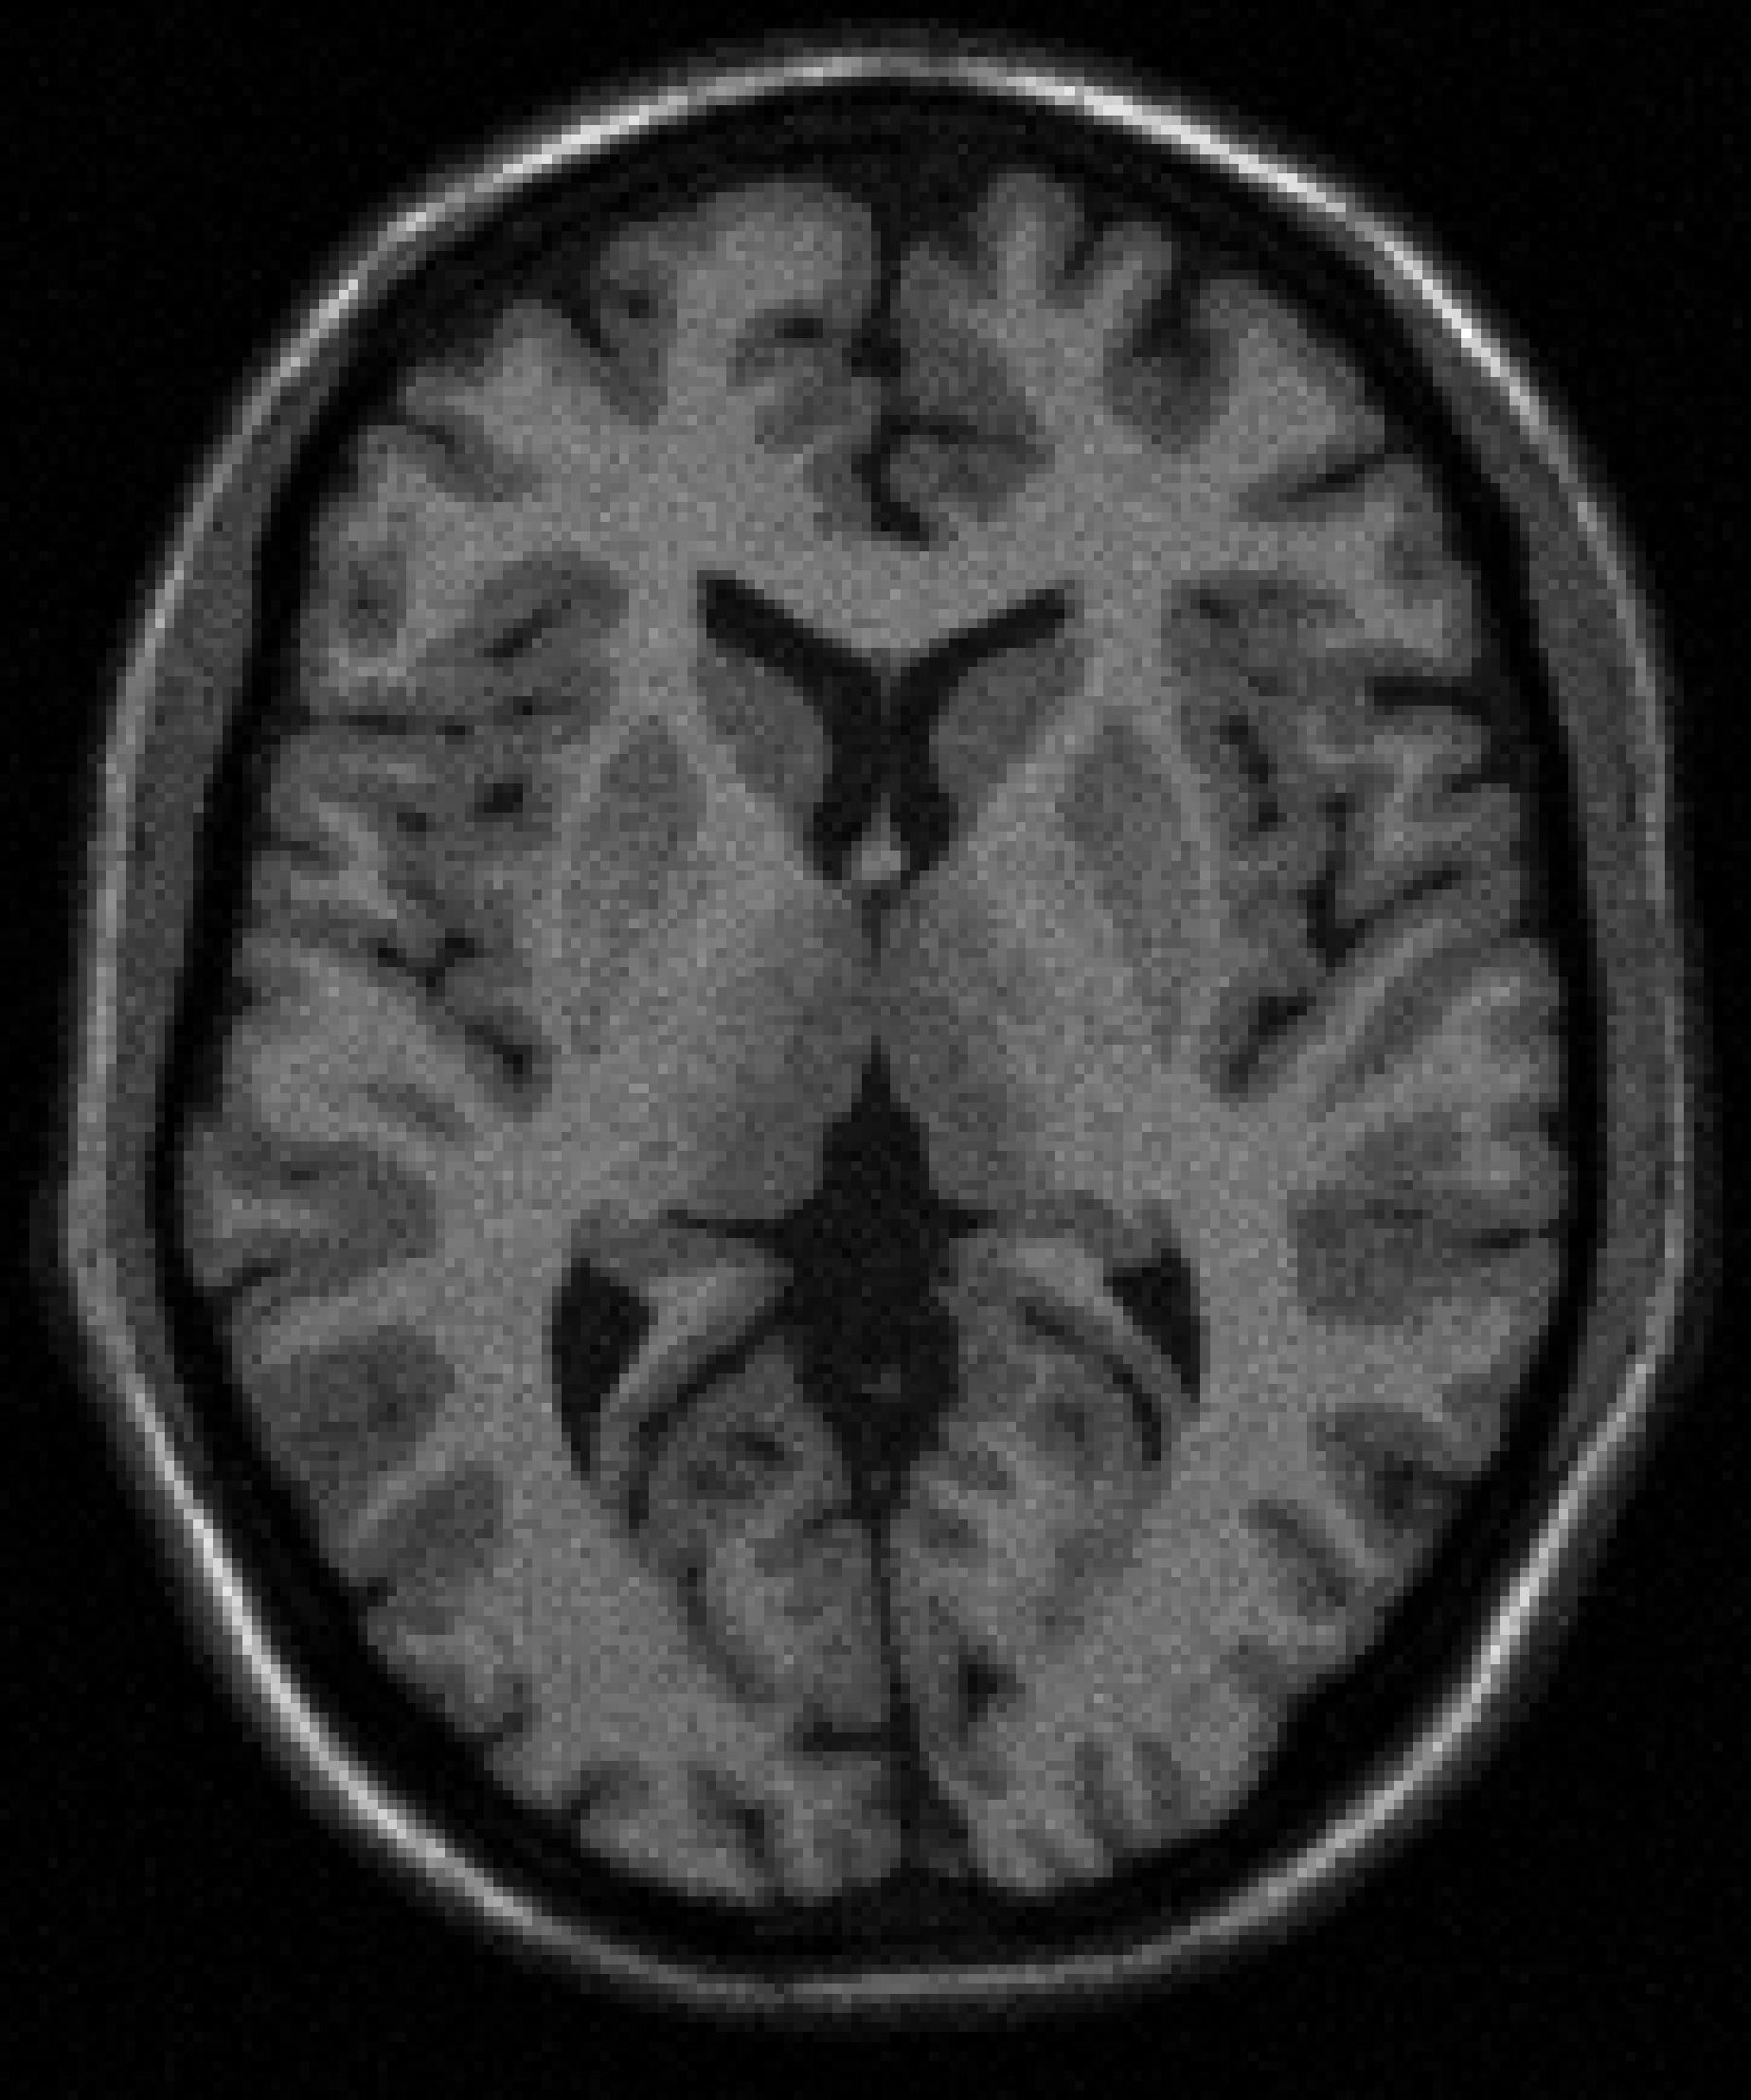
\includegraphics[width=\textwidth]{Figuras/ImageA_exp_gamma=1.5.png}
            \caption{$\gamma = 1.5$} 
         \end{subfigure}
         \begin{subfigure}[h]{0.32\linewidth}
            \centering
            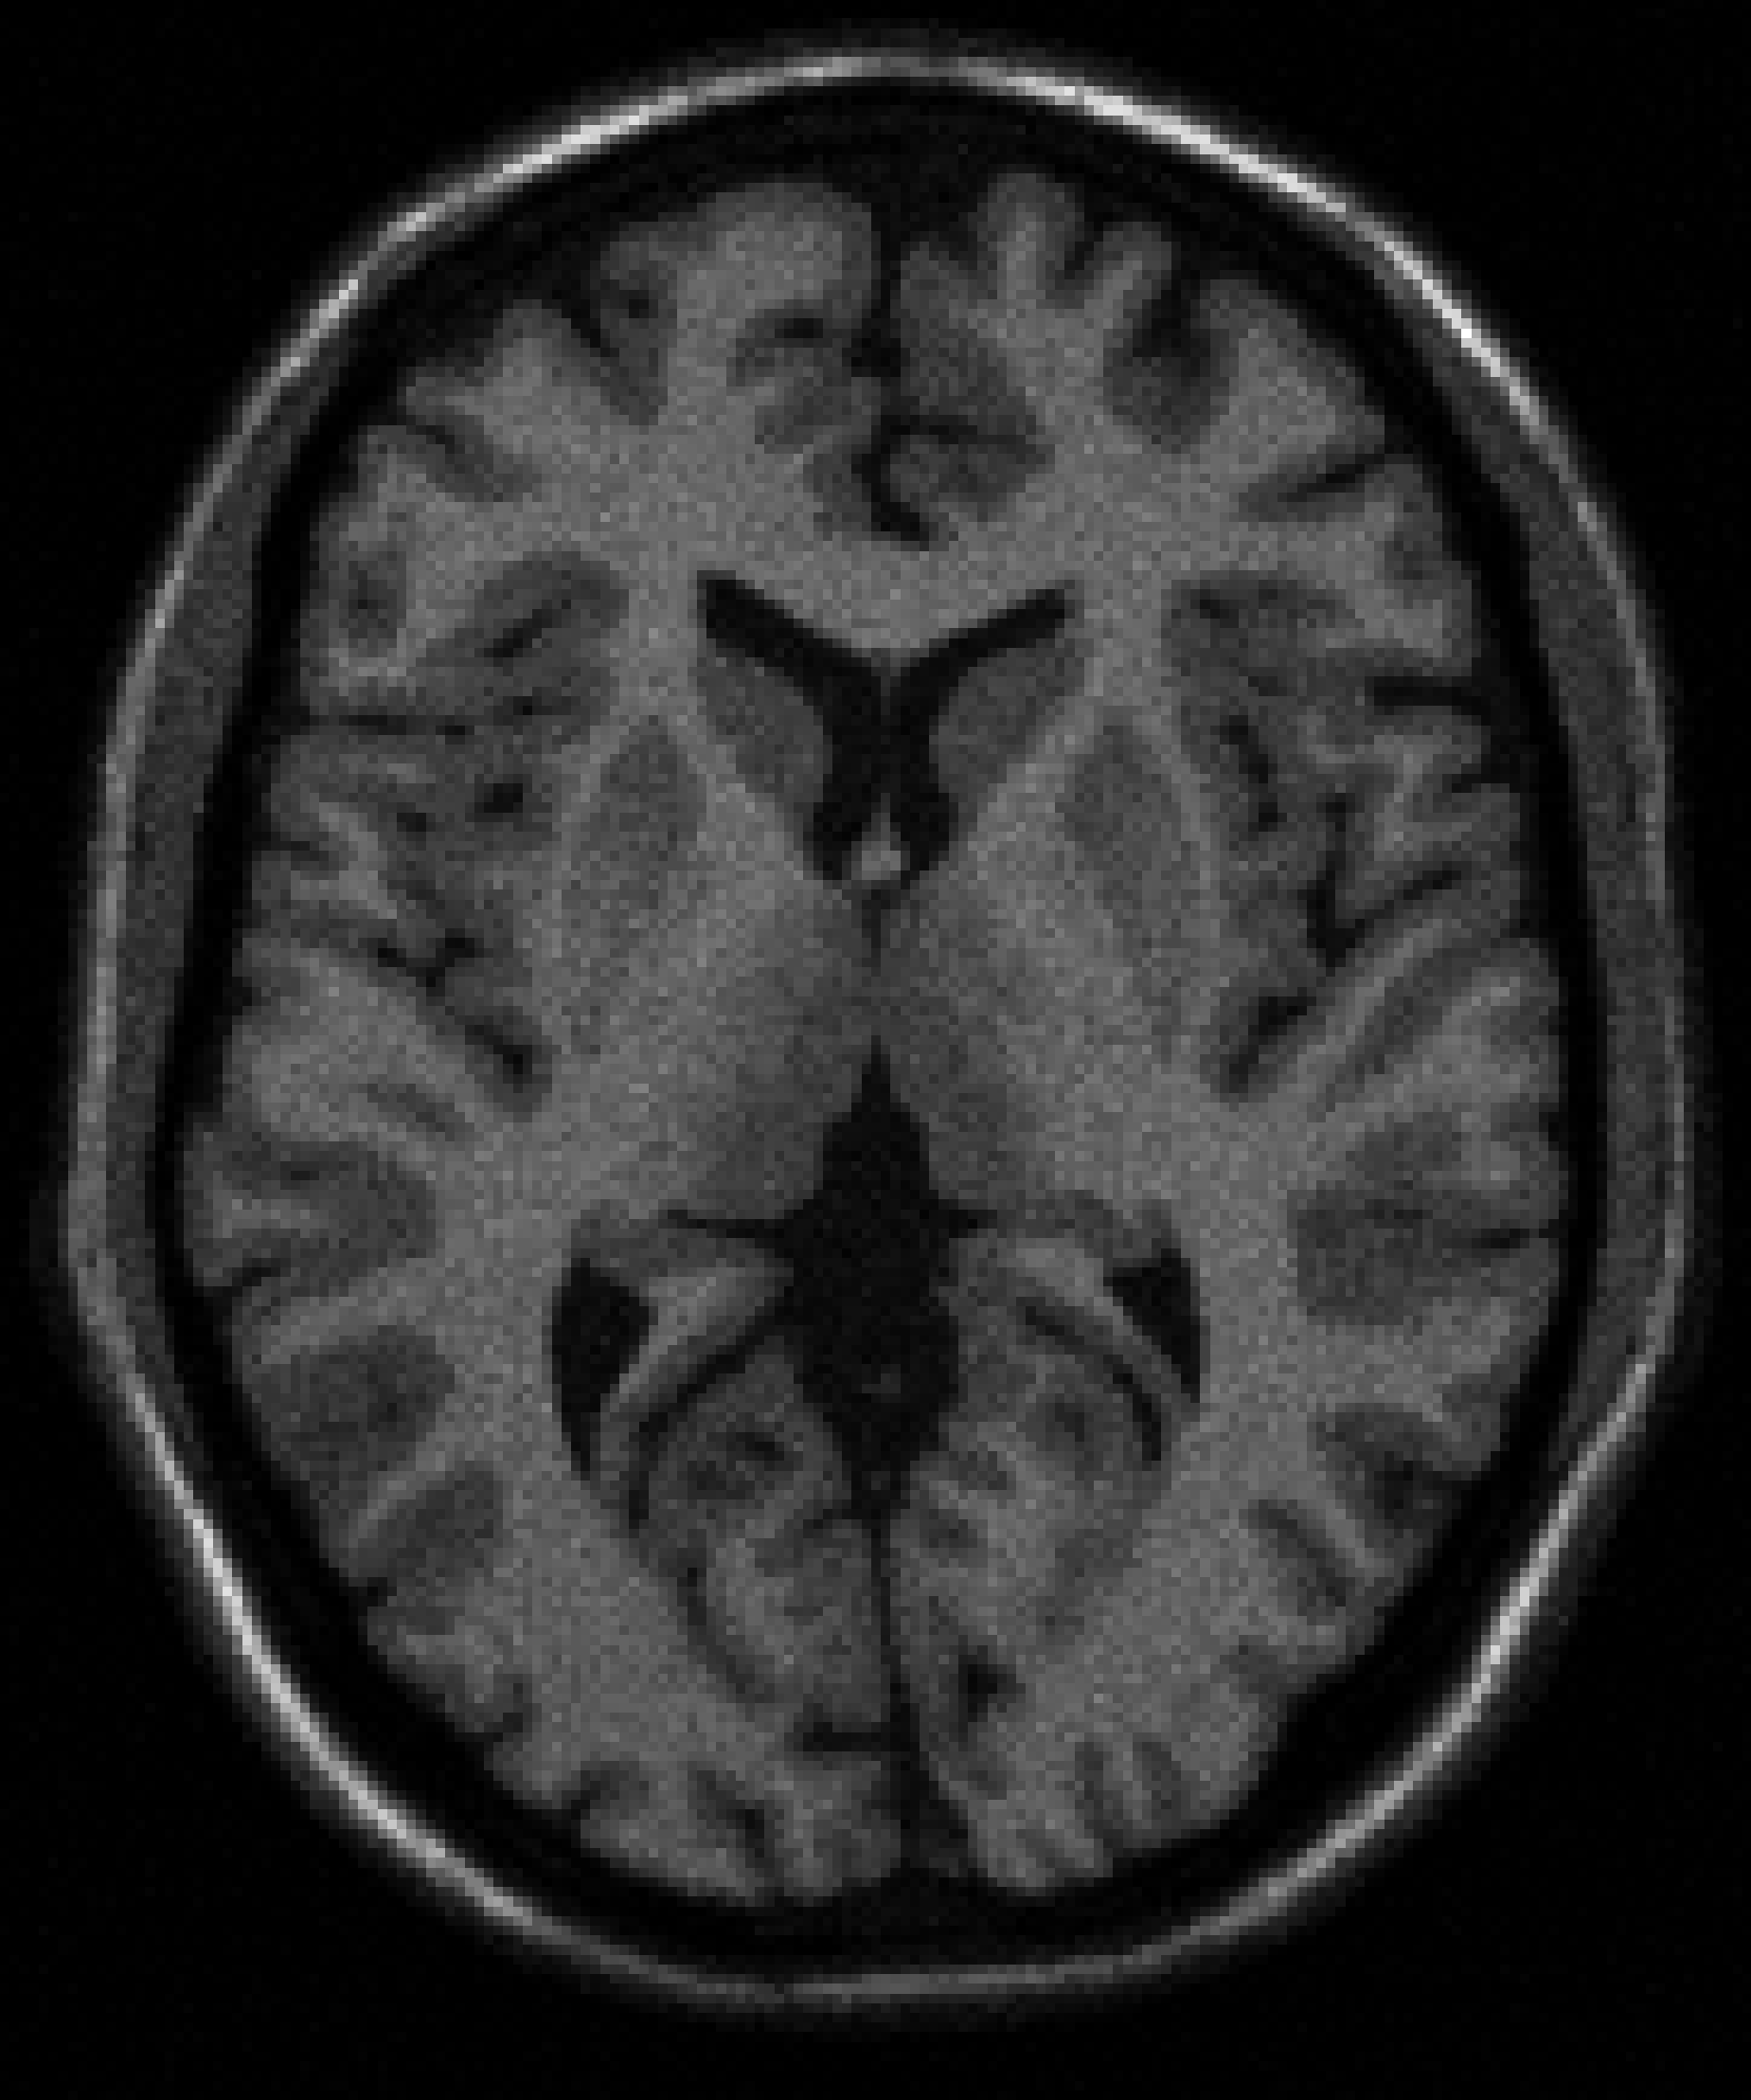
\includegraphics[width=\textwidth]{Figuras/ImageA_exp_gamma=1.75.png}
            \caption{$\gamma = 1.75$} 
         \end{subfigure}
    \caption{Transformación $\gamma$ aplicada a la imagenA original.}
    \label{fig:Exptrans}
\end{figure}

Por último, en las Figs. \ref{fig:EQ_sustraction}, \ref{fig:binary_sustraction}, \ref{fig:Exptrans0.5_sustraction} y \ref{fig:Exptrans1.75_sustraction} se muestran la resta de la imagenA original con la imagenA luego de aplicarle transformaciones de ecualización, binarización y $\gamma$ con $\gamma = 0.5,1.75$ respectivamente.

\begin{figure}[h]
    \centering
        \begin{subfigure}[h]{0.24\linewidth}
            \centering
            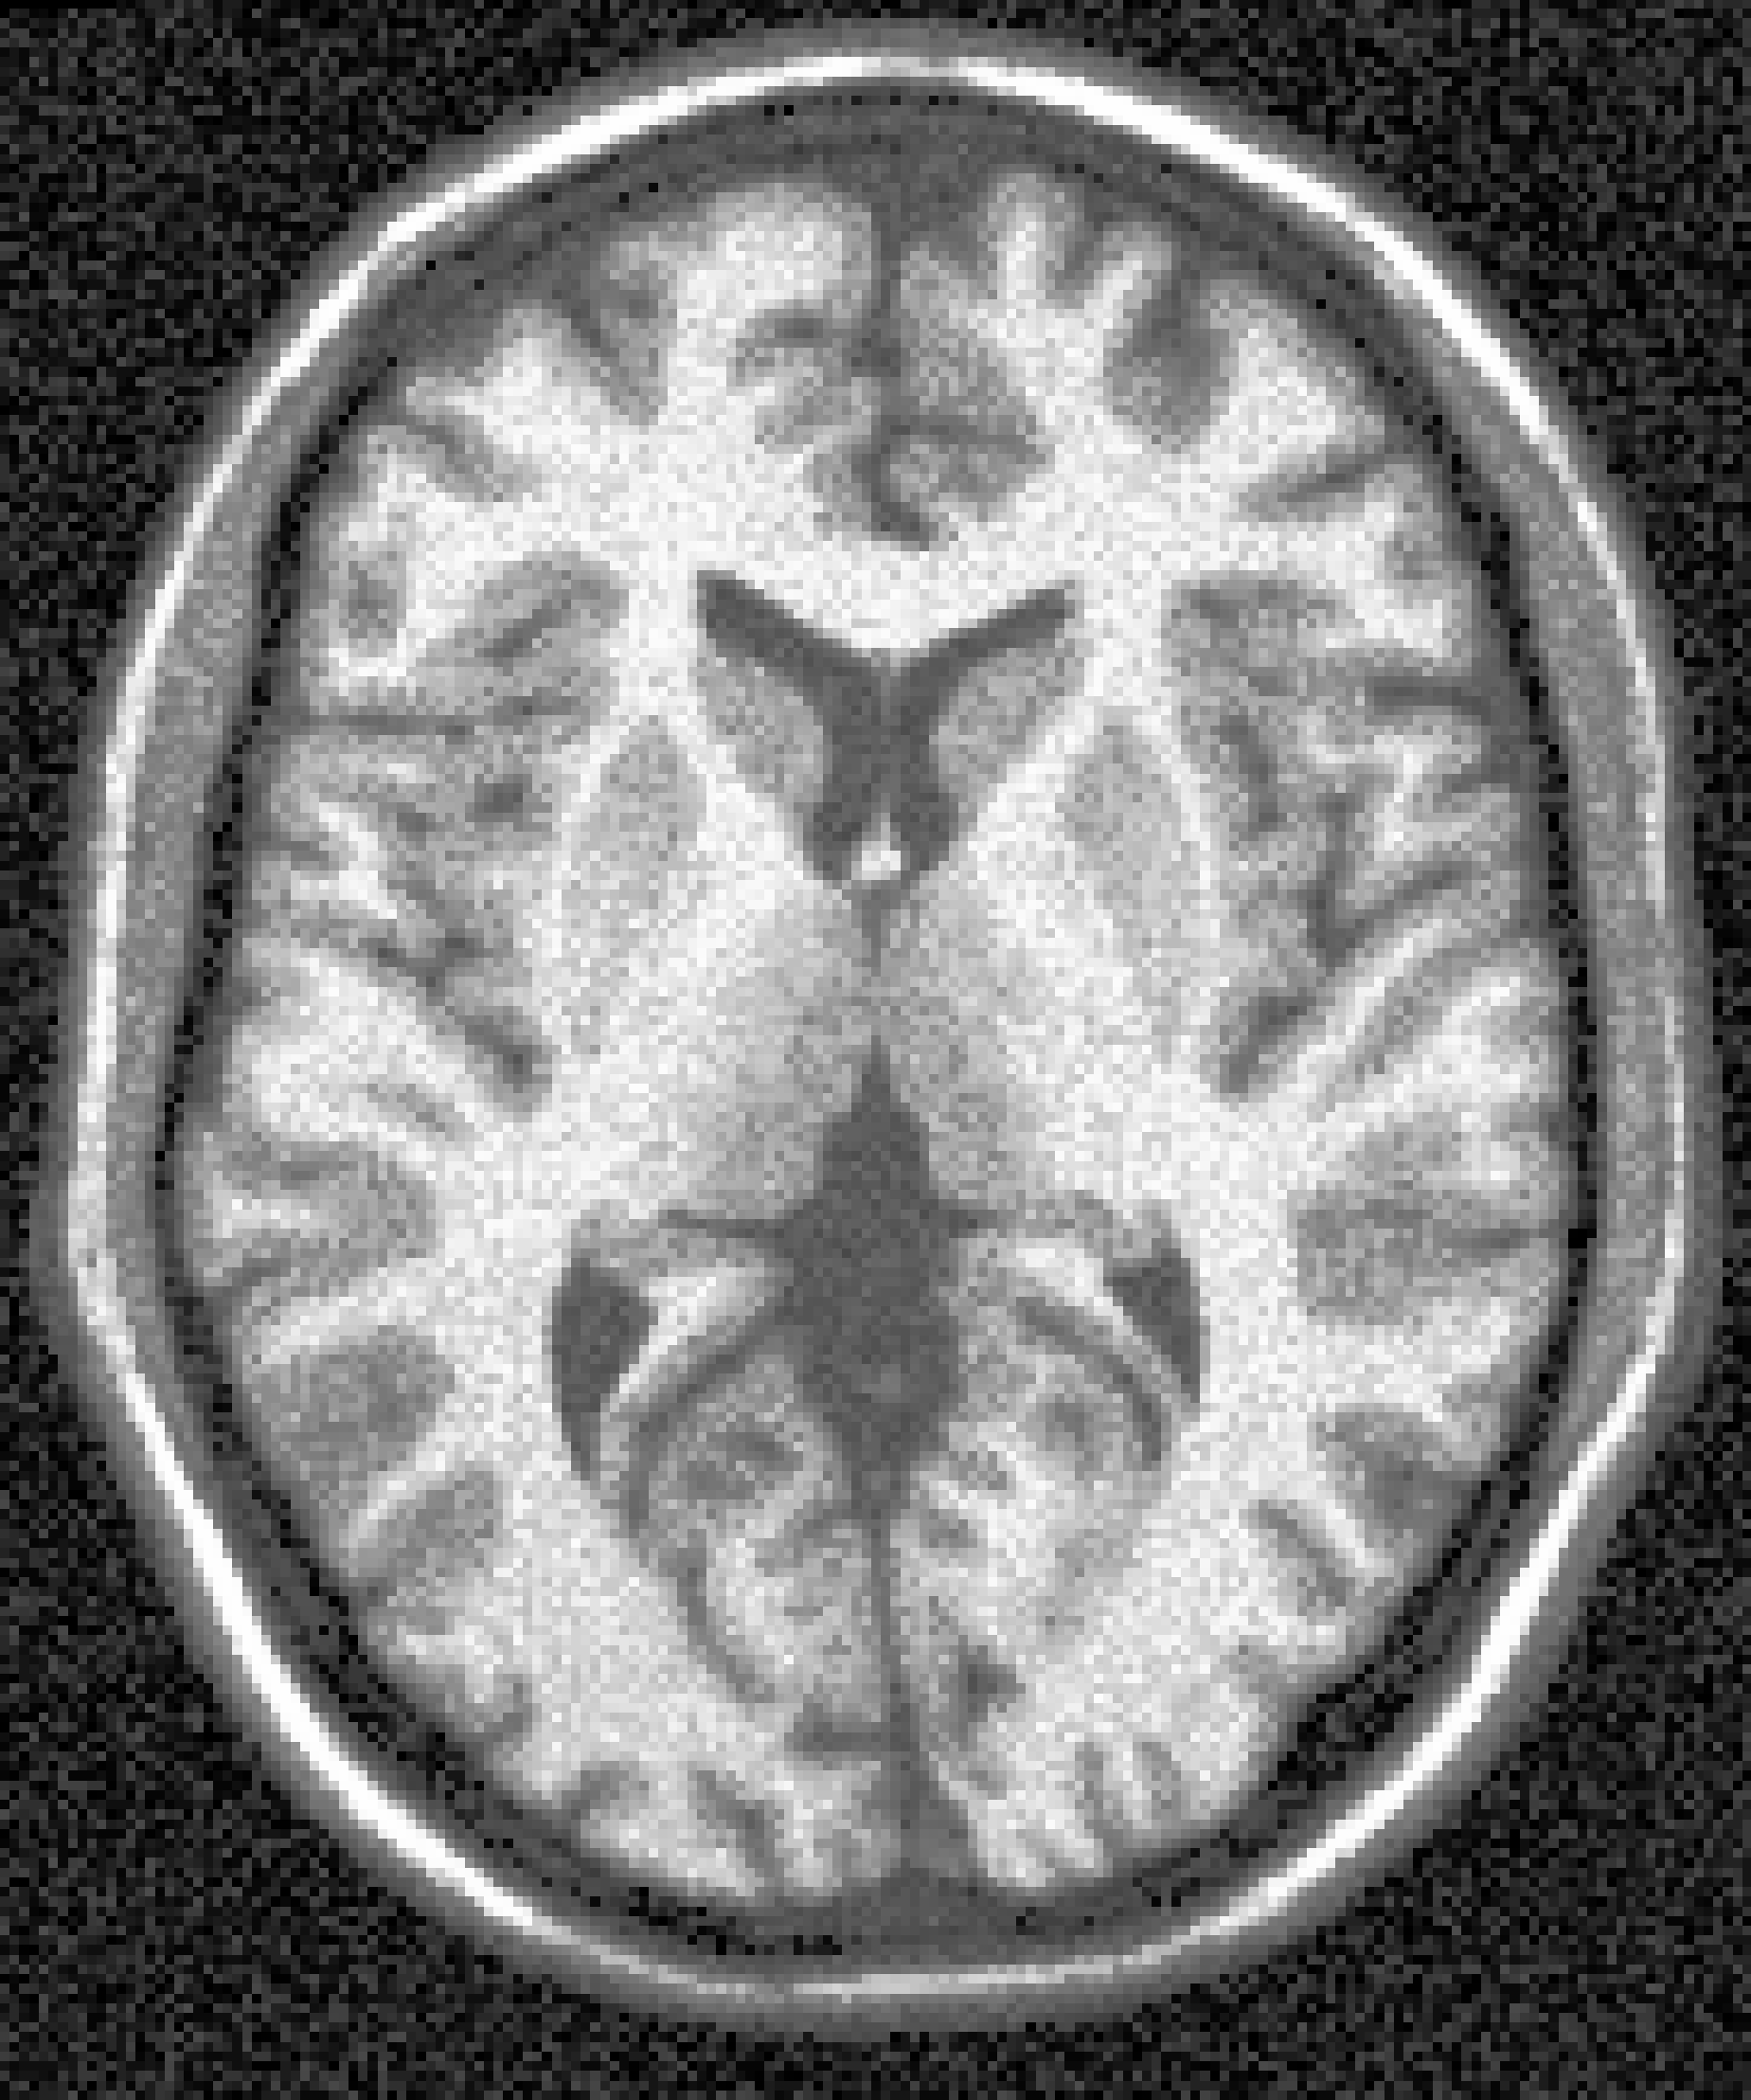
\includegraphics[width=\textwidth]{Figuras/ImageA_EQ}
        \end{subfigure}
        \begin{subfigure}[h]{0.24\linewidth}
            \centering
            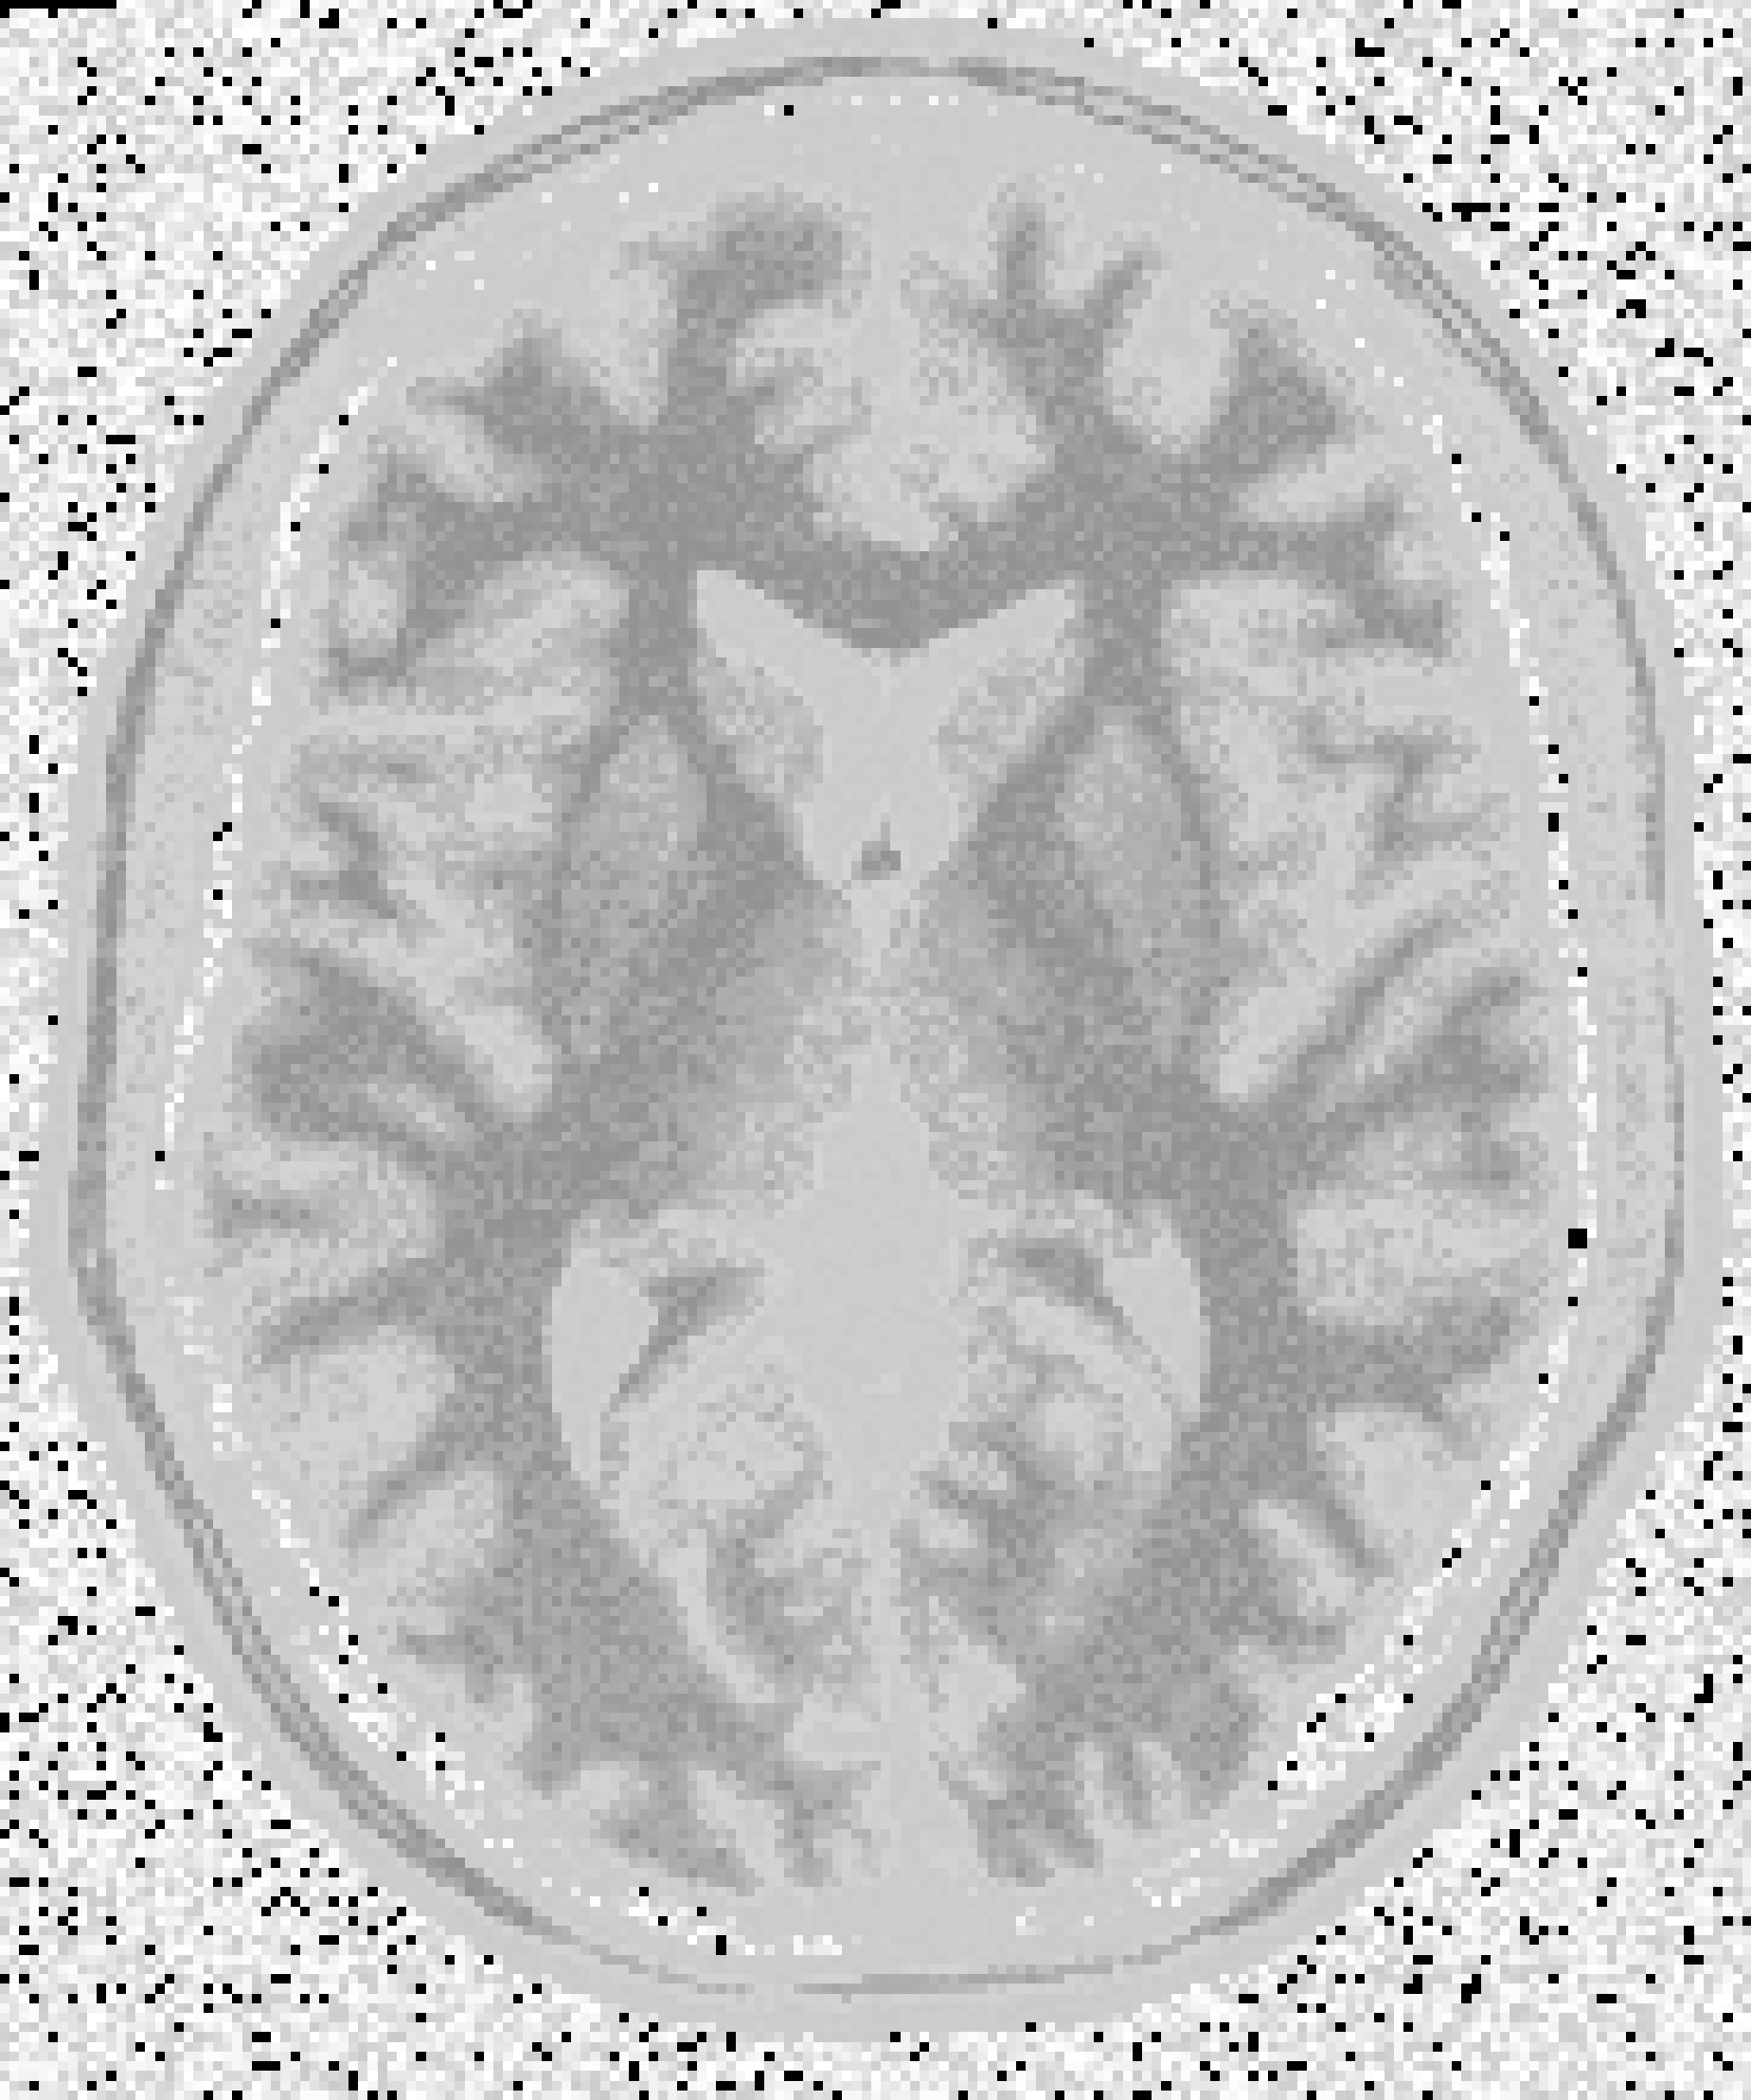
\includegraphics[width=\textwidth]{Figuras/sustraction_EQ.png}
        \end{subfigure}
                \caption{Diferencia entre la imagen original y la imagen ecualizada.}
                \label{fig:EQ_sustraction}
         \begin{subfigure}[h]{0.24\linewidth}
            \centering
            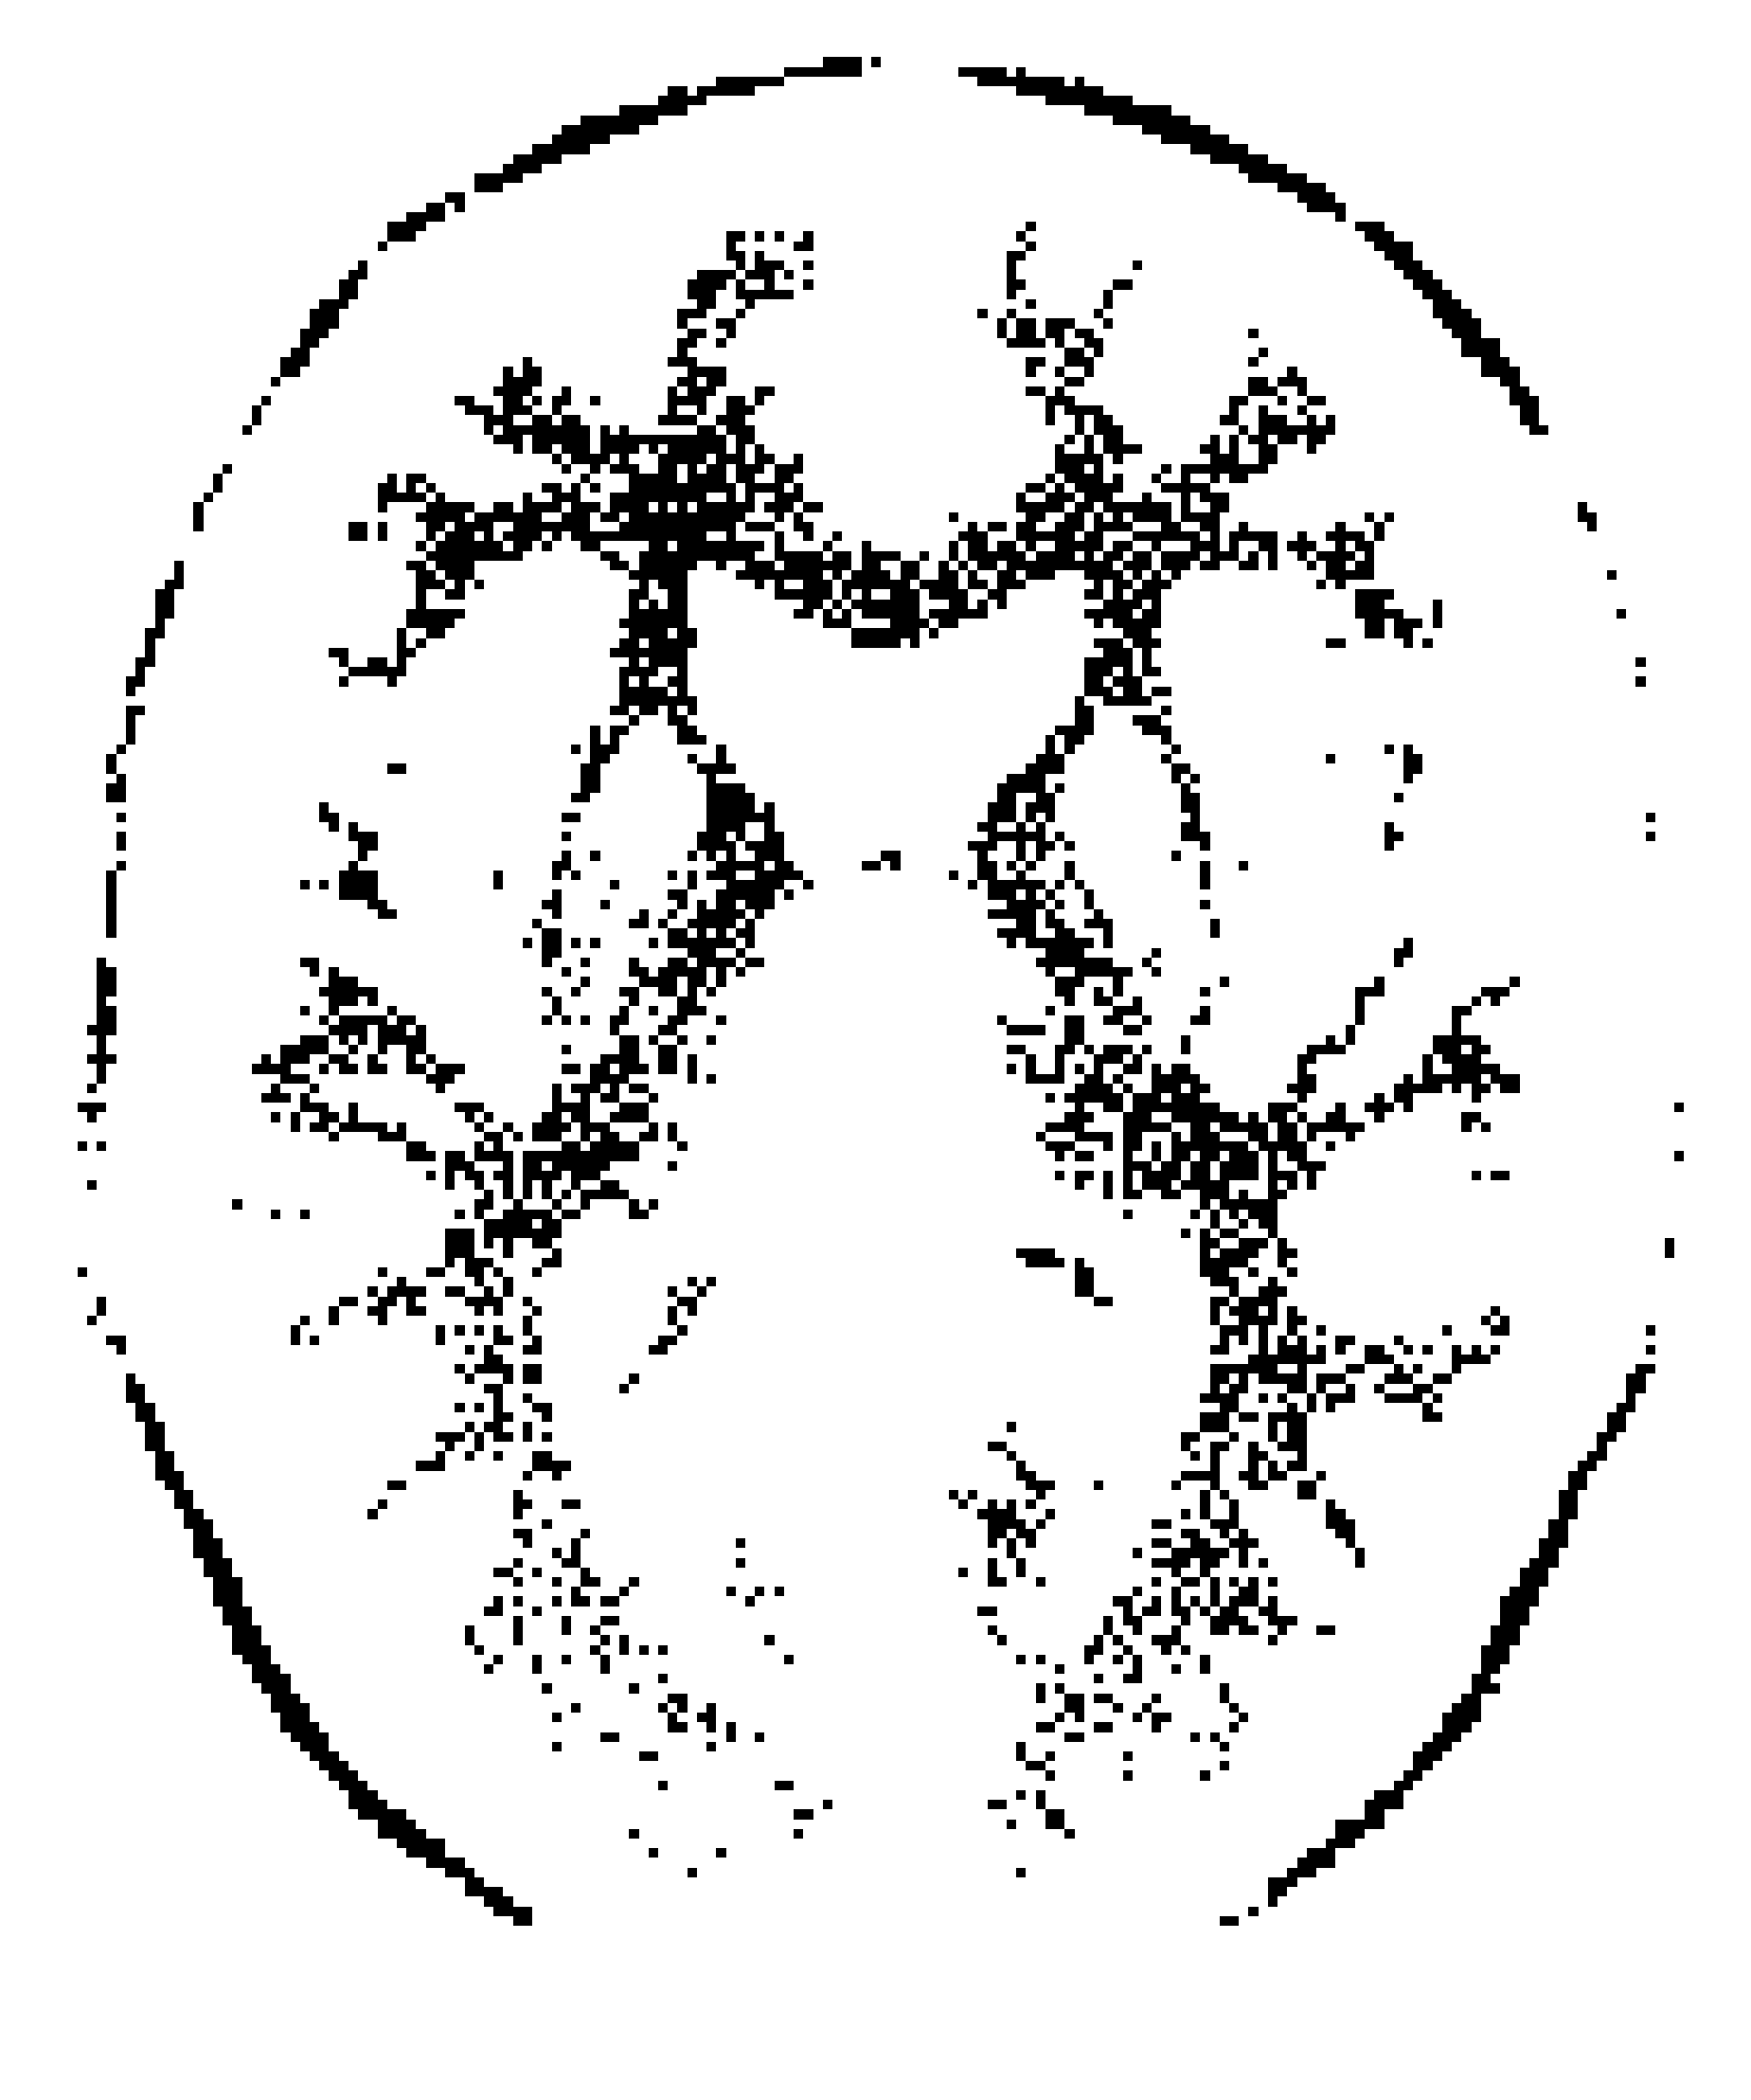
\includegraphics[width=\textwidth]{Figuras/ImageA_binary.png}
         \end{subfigure}
         \begin{subfigure}[h]{0.24\linewidth}
            \centering
            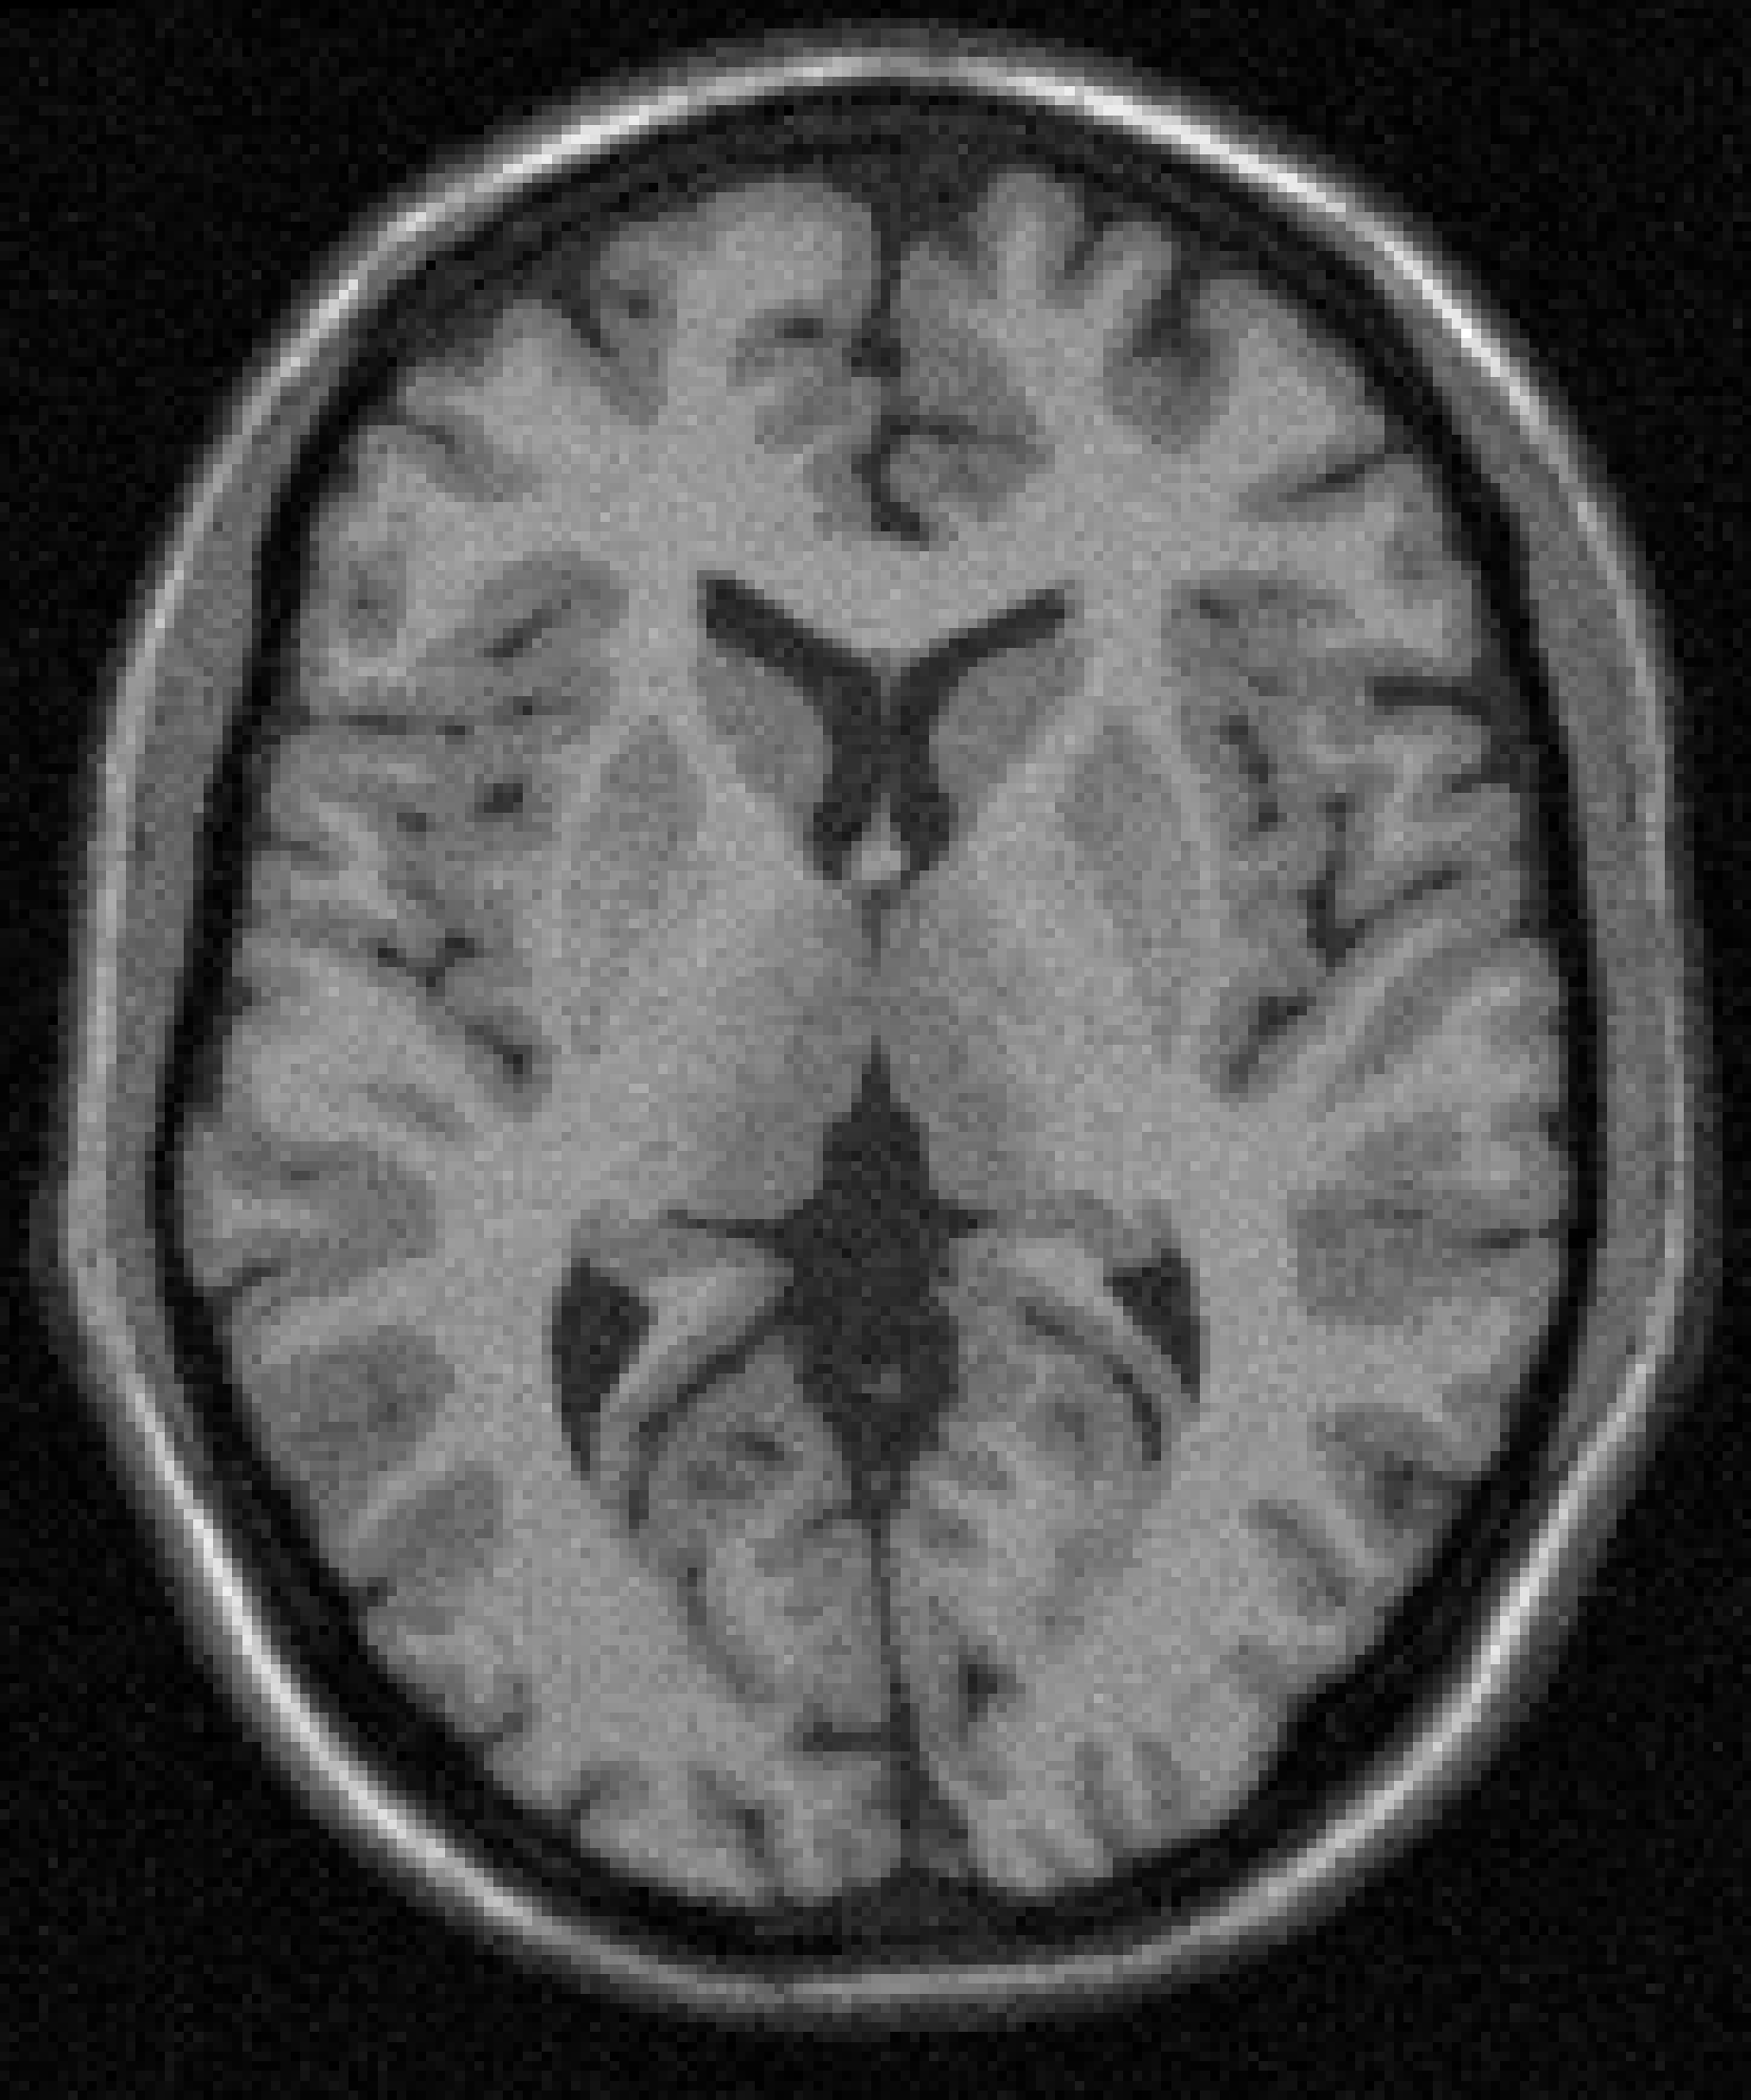
\includegraphics[width=\textwidth]{Figuras/sustraction_binary.png}
         \end{subfigure}
                 \caption{Difererencia entre la imagen original y la imagen binarizada.} 
                 \label{fig:binary_sustraction}
        \begin{subfigure}[h]{0.24\linewidth}
            \centering
            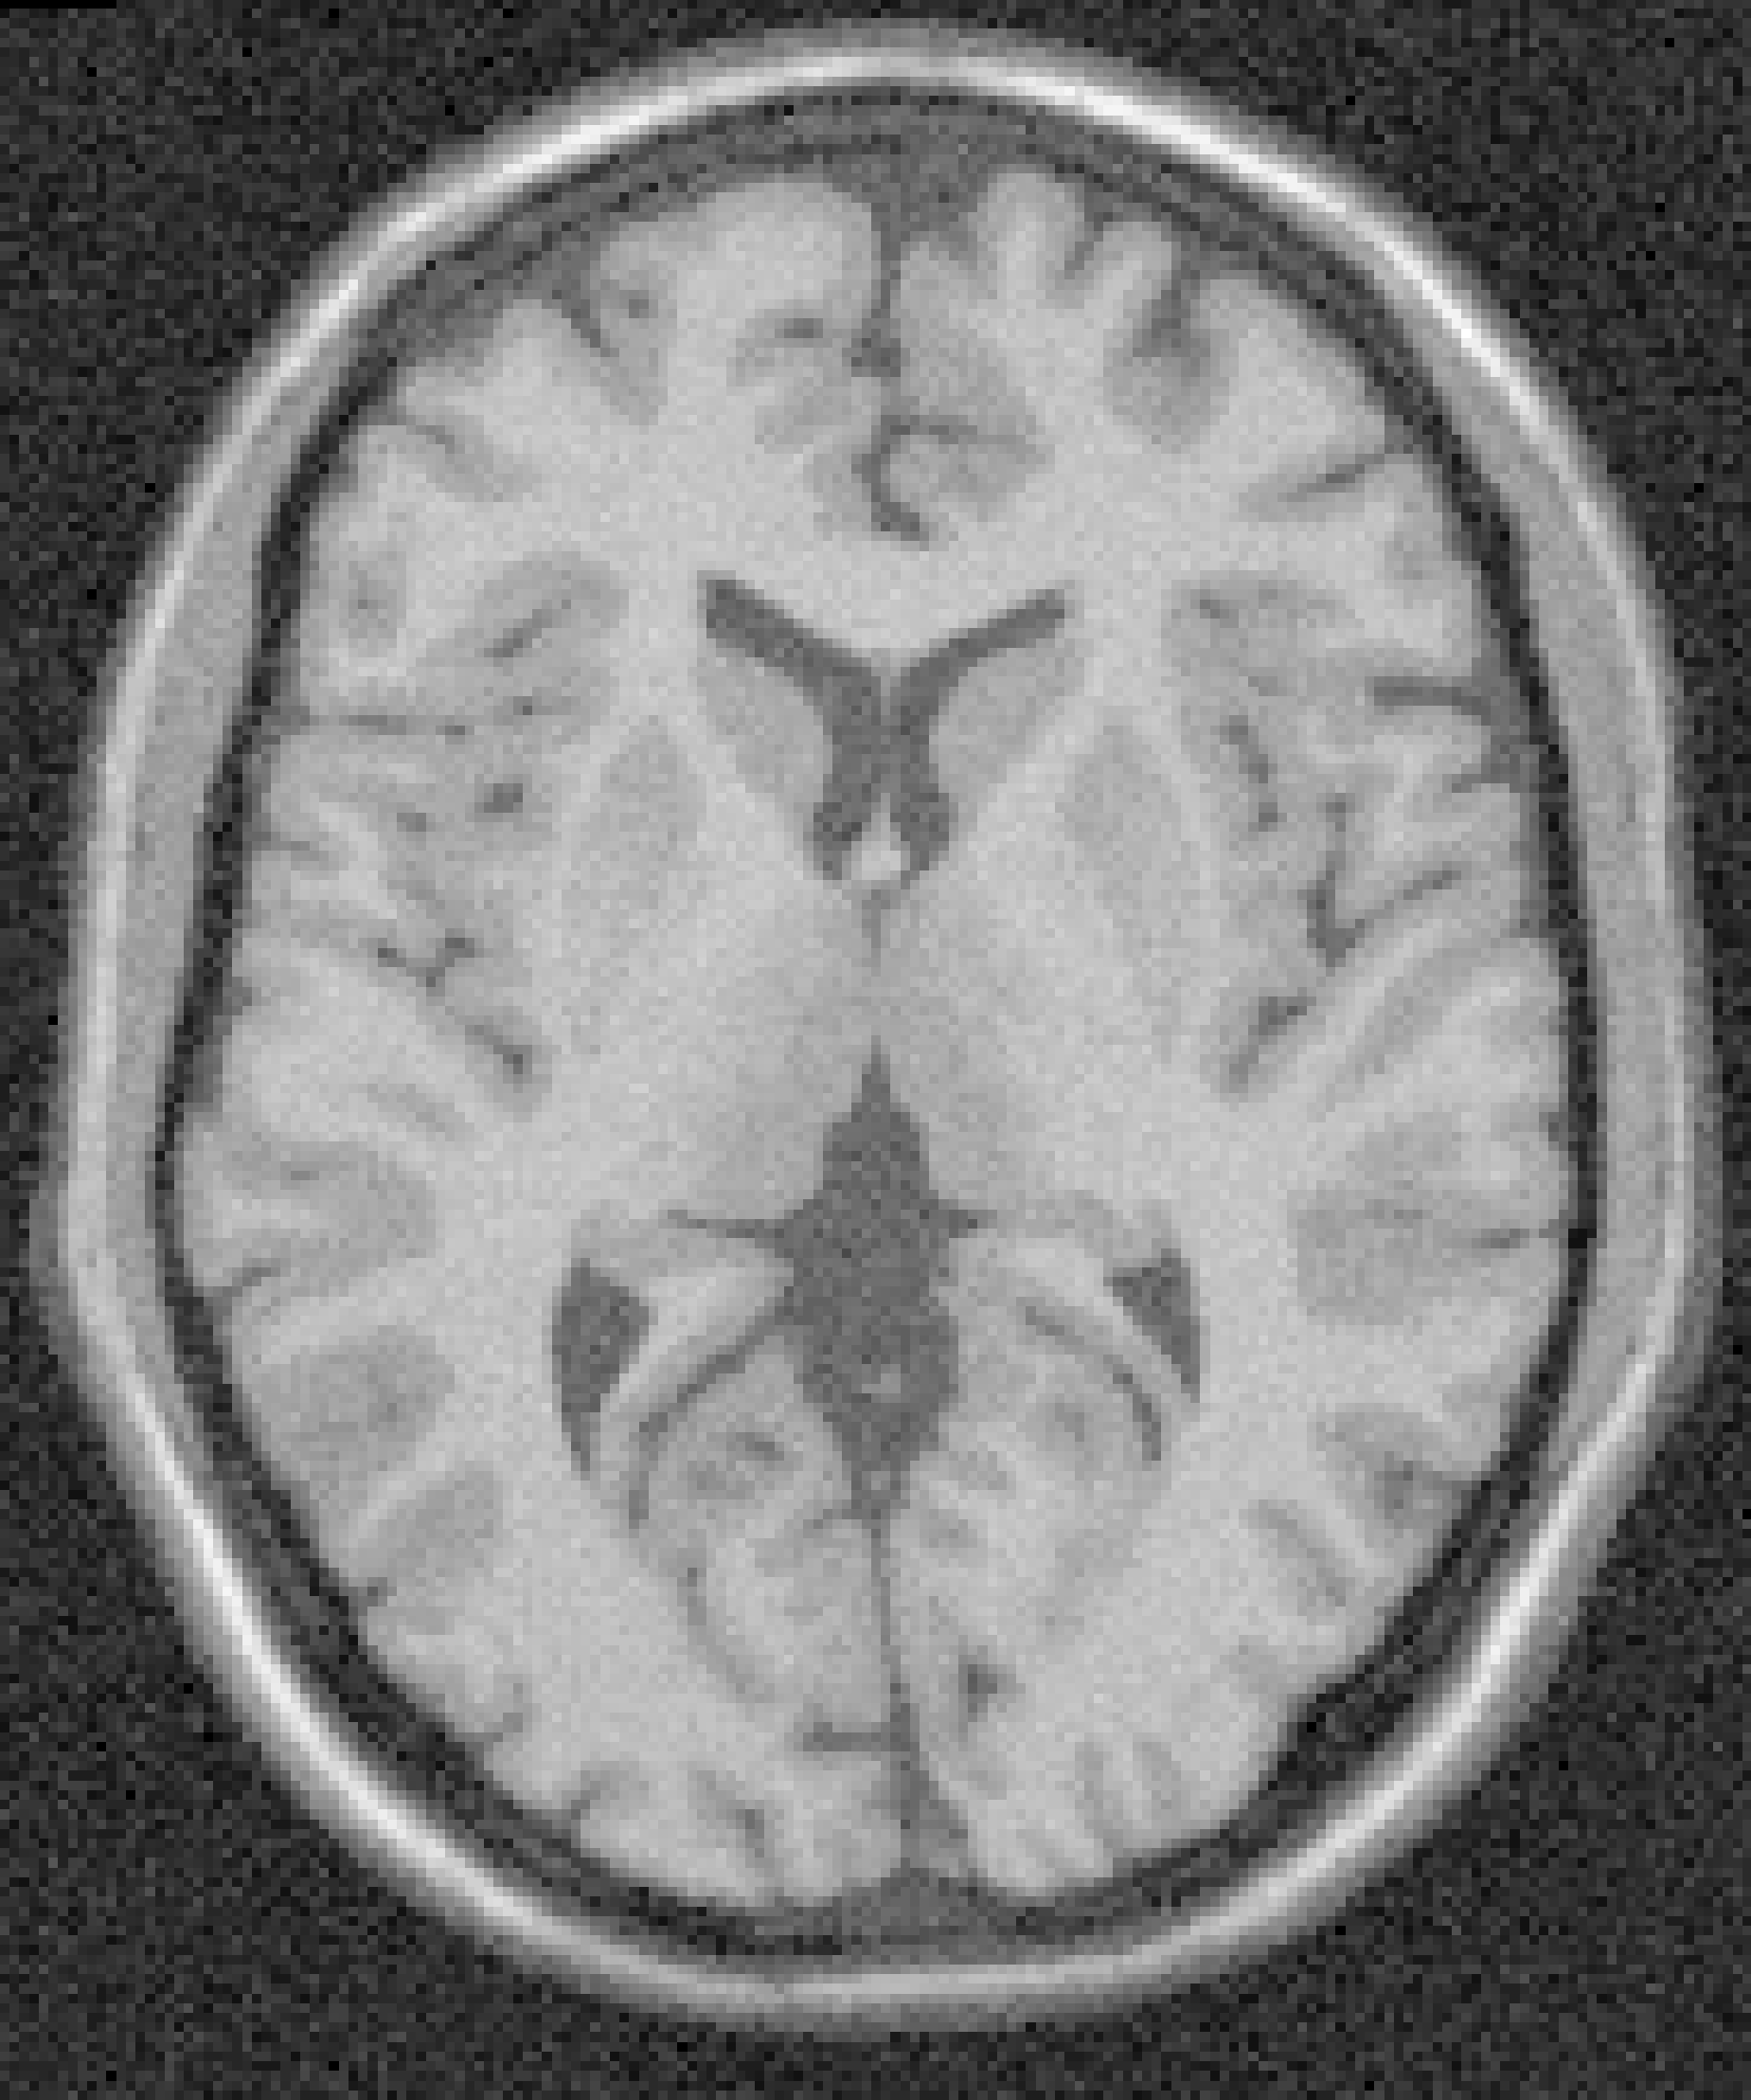
\includegraphics[width=\textwidth]{Figuras/ImageA_exp_gamma=0.5.png}
        \end{subfigure}
        \begin{subfigure}[h]{0.24\linewidth}
            \centering
            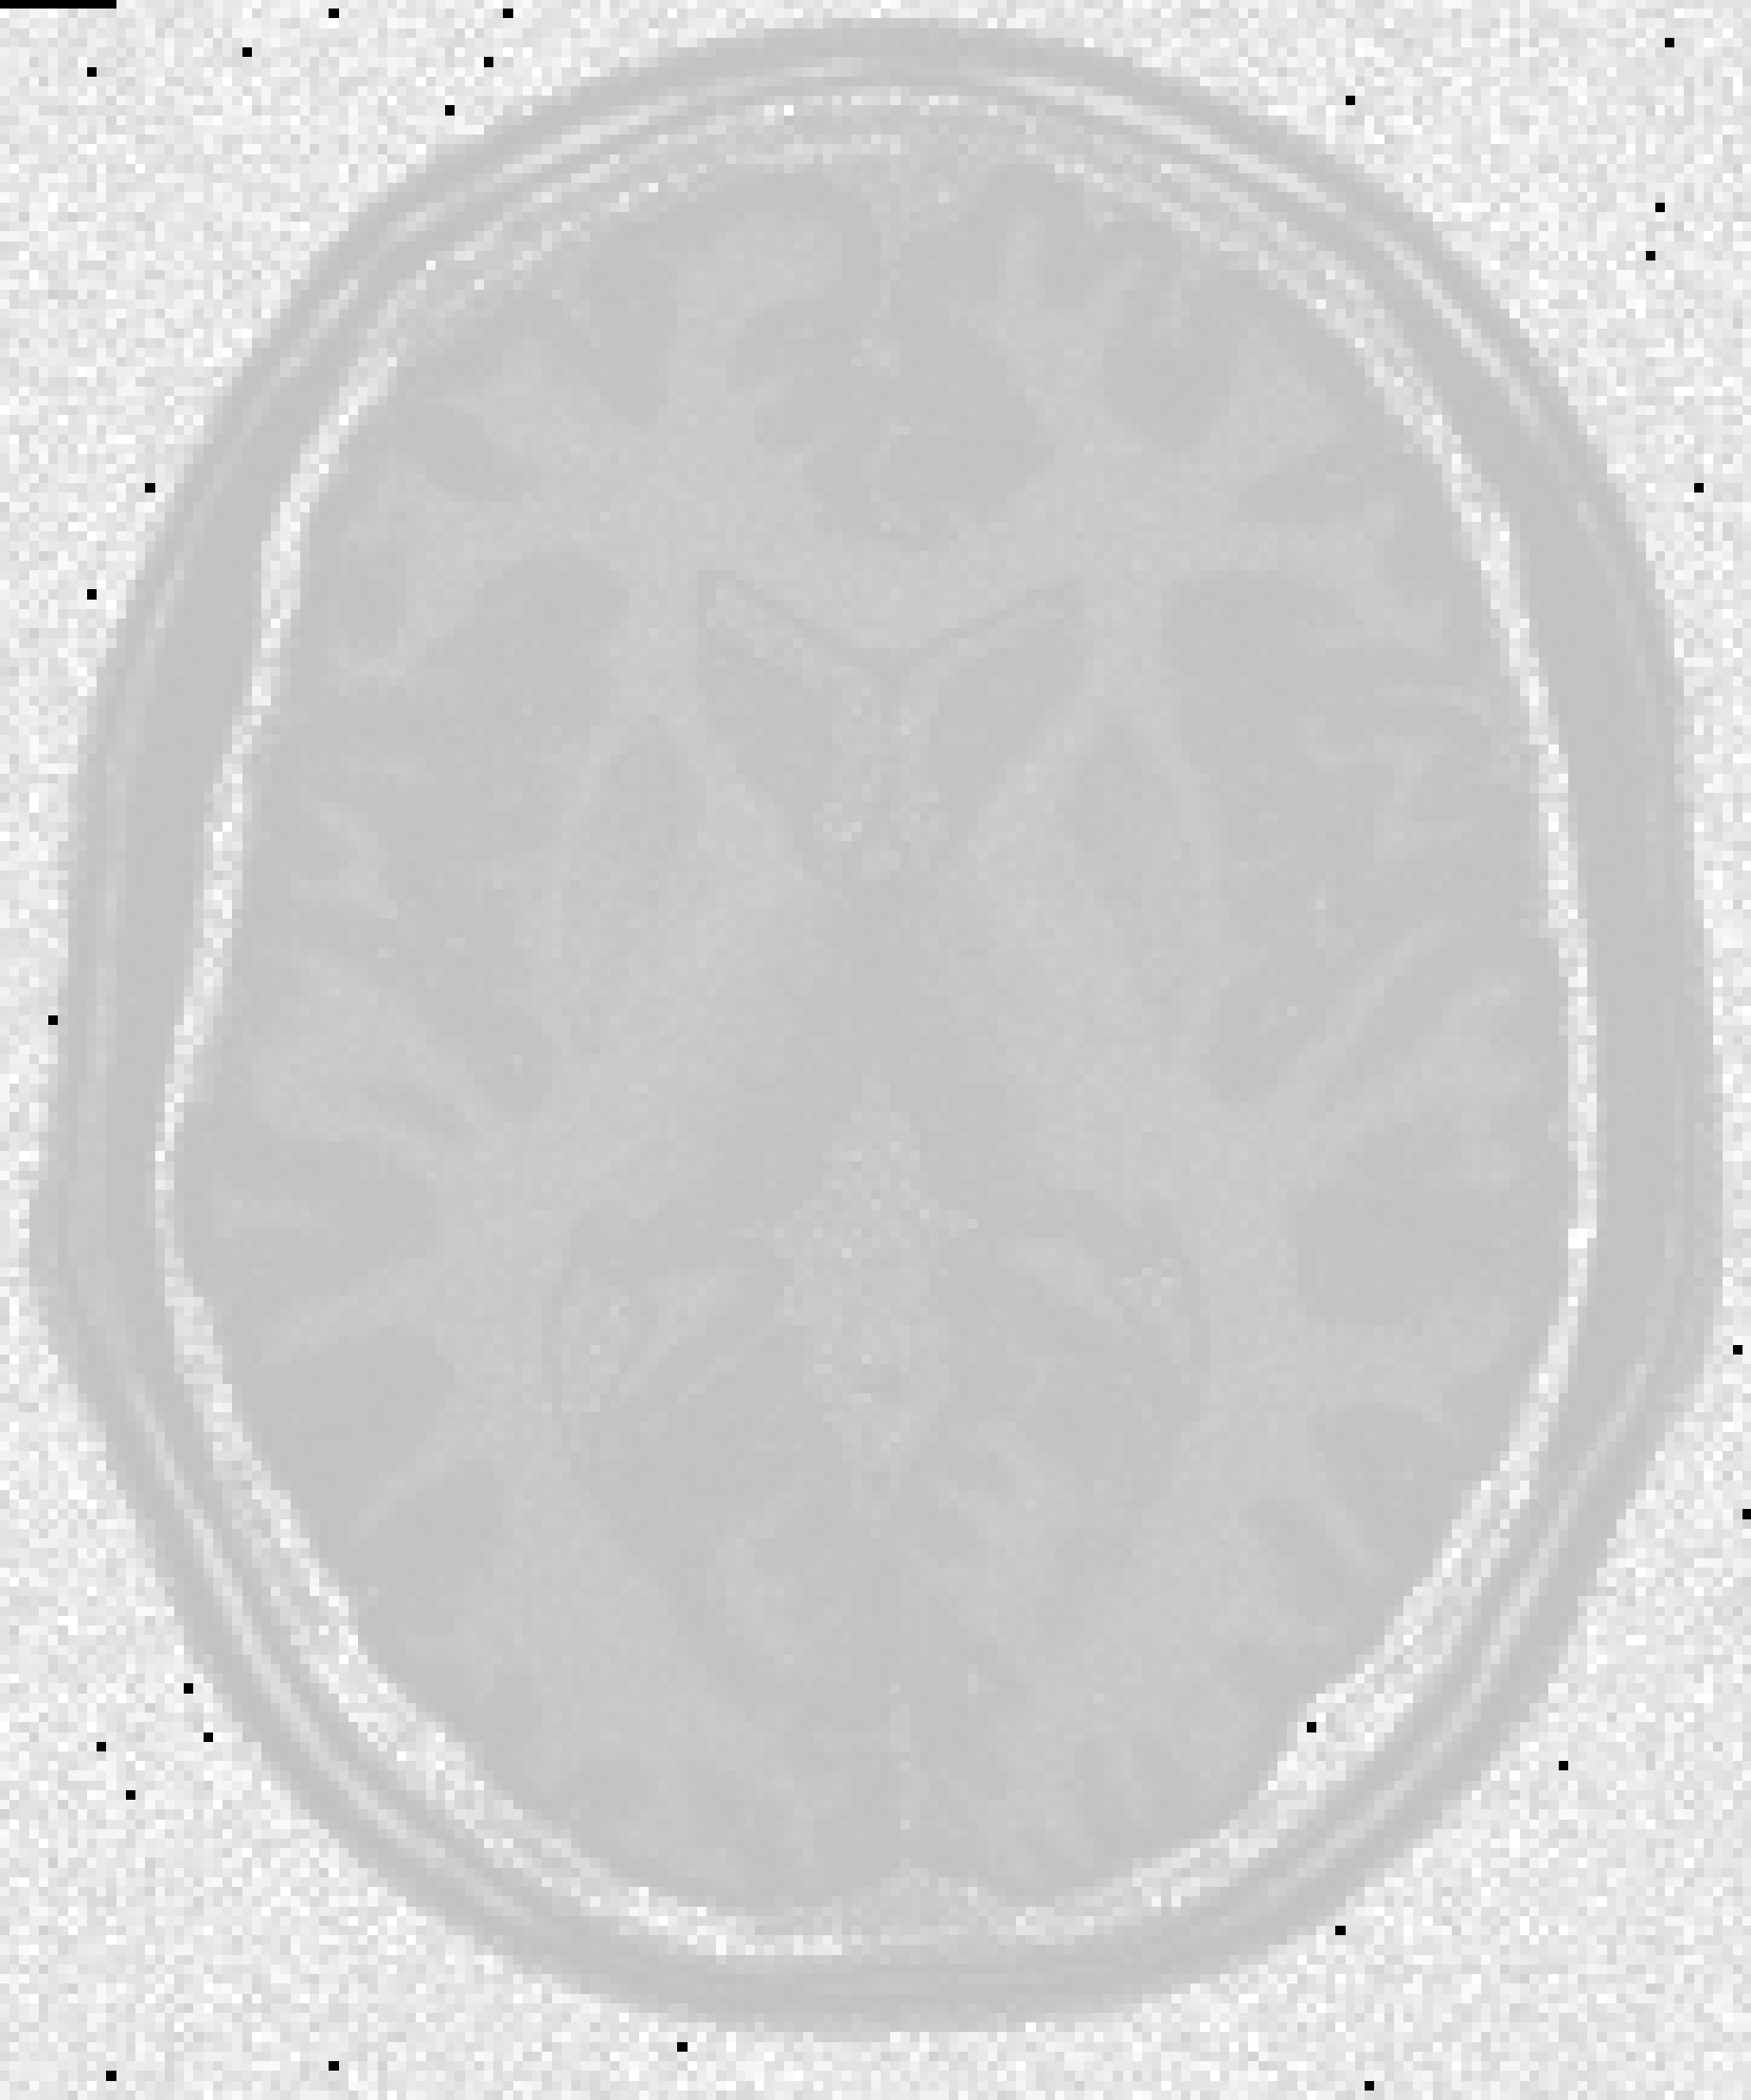
\includegraphics[width=\textwidth]{Figuras/sustraction_exp_gamma=0.5.png}
        \end{subfigure}
                \caption{Diferencia entre la imagen original y la imagen transformada con $\gamma = 0.5$.}
                \label{fig:Exptrans0.5_sustraction}
        \begin{subfigure}[h]{0.24\linewidth}
            \centering
            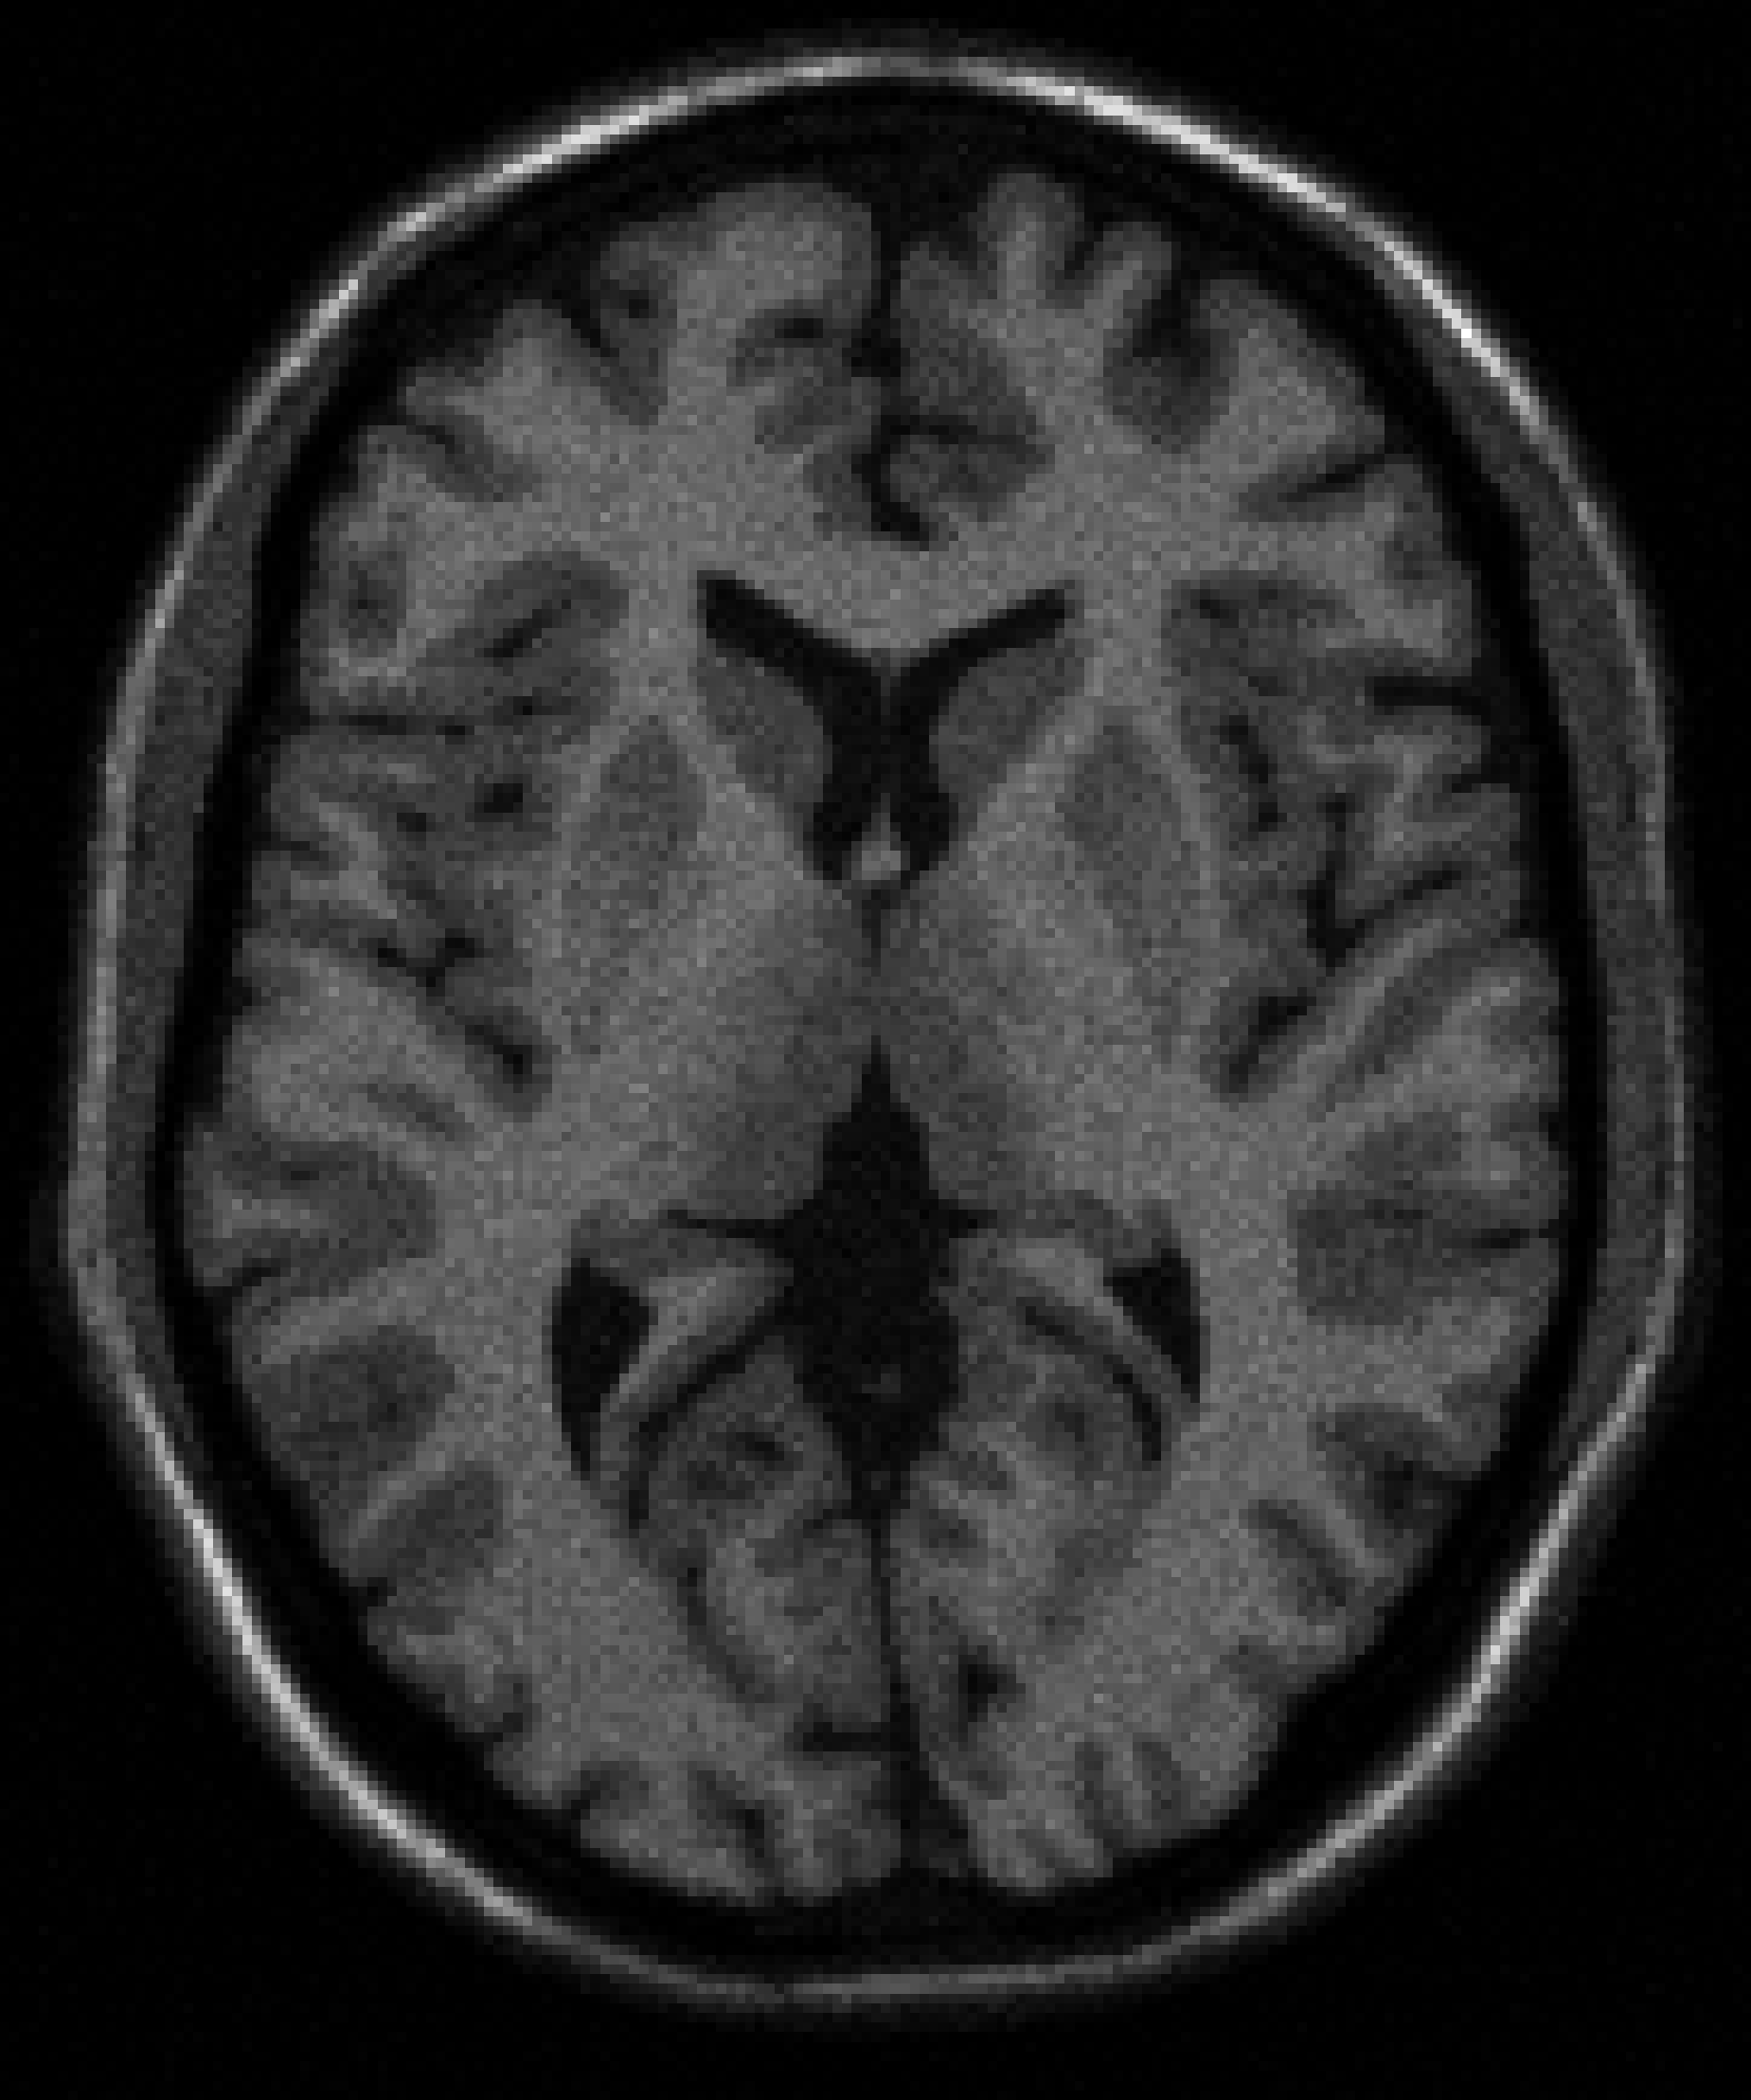
\includegraphics[width=\textwidth]{Figuras/ImageA_exp_gamma=1.75.png}
        \end{subfigure}
        \begin{subfigure}[h]{0.24\linewidth}
            \centering
            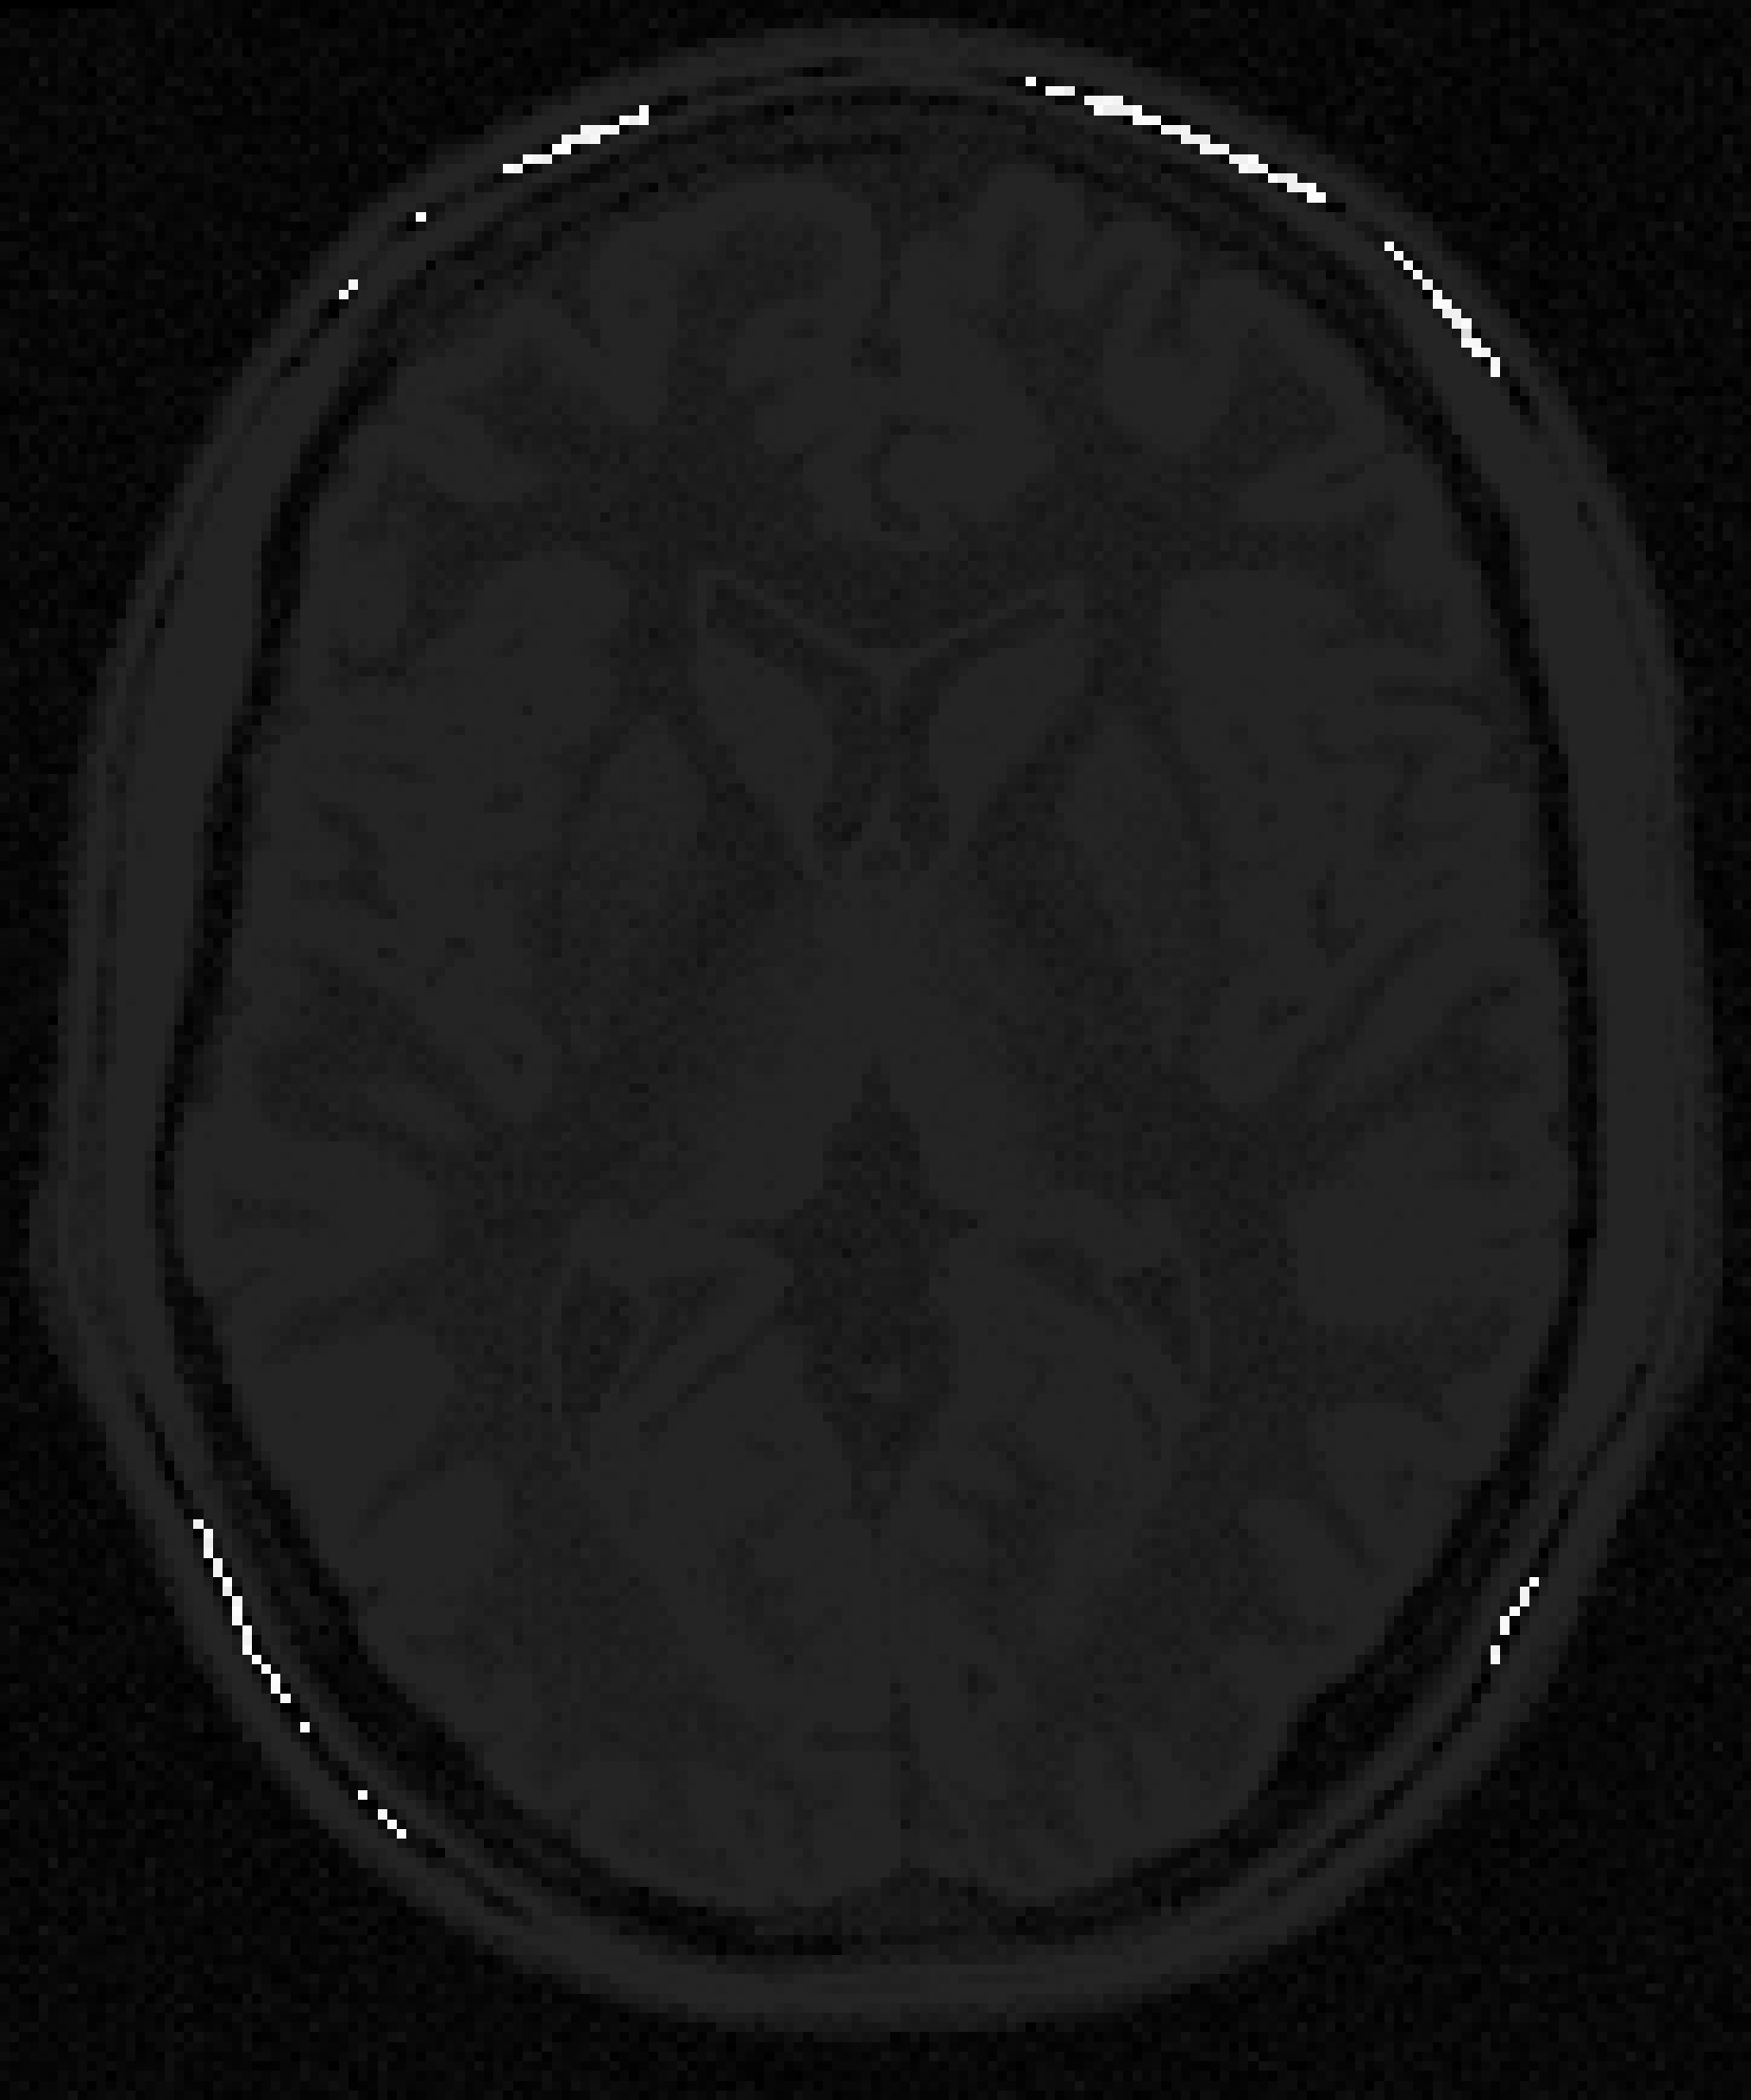
\includegraphics[width=\textwidth]{Figuras/sustraction_exp_gamma=1.75.png}
        \end{subfigure}
                \caption{Diferencia entre la imagen original y la imagen transformada con $\gamma = 1.75$.}
                \label{fig:Exptrans1.75_sustraction}
\end{figure}

\section{Interpolación \label{sec:ej3}}

\vspace{0.3cm}

Se tomó la imagen C de tamaño $128\times128$ pixels$^2$ y se interpoló utilizando el método de vecinos más cercanos y bilineal implementados en python para obtener imágenes de $32\times32$, $64\times64$, $256\times256$ y $1024\times1024$. La implementación de ambas técnicas se realizó en python. Los resultados se muestran en la Fig. \ref{fig:Interpolate}. Se observa que la interpolación bilineal es más suave en la transición de la escala de grises que la interpolación por vecinos más cercanos.

\begin{figure}[h]
    \centering
        \begin{subfigure}[h]{0.24\linewidth}
            \centering
            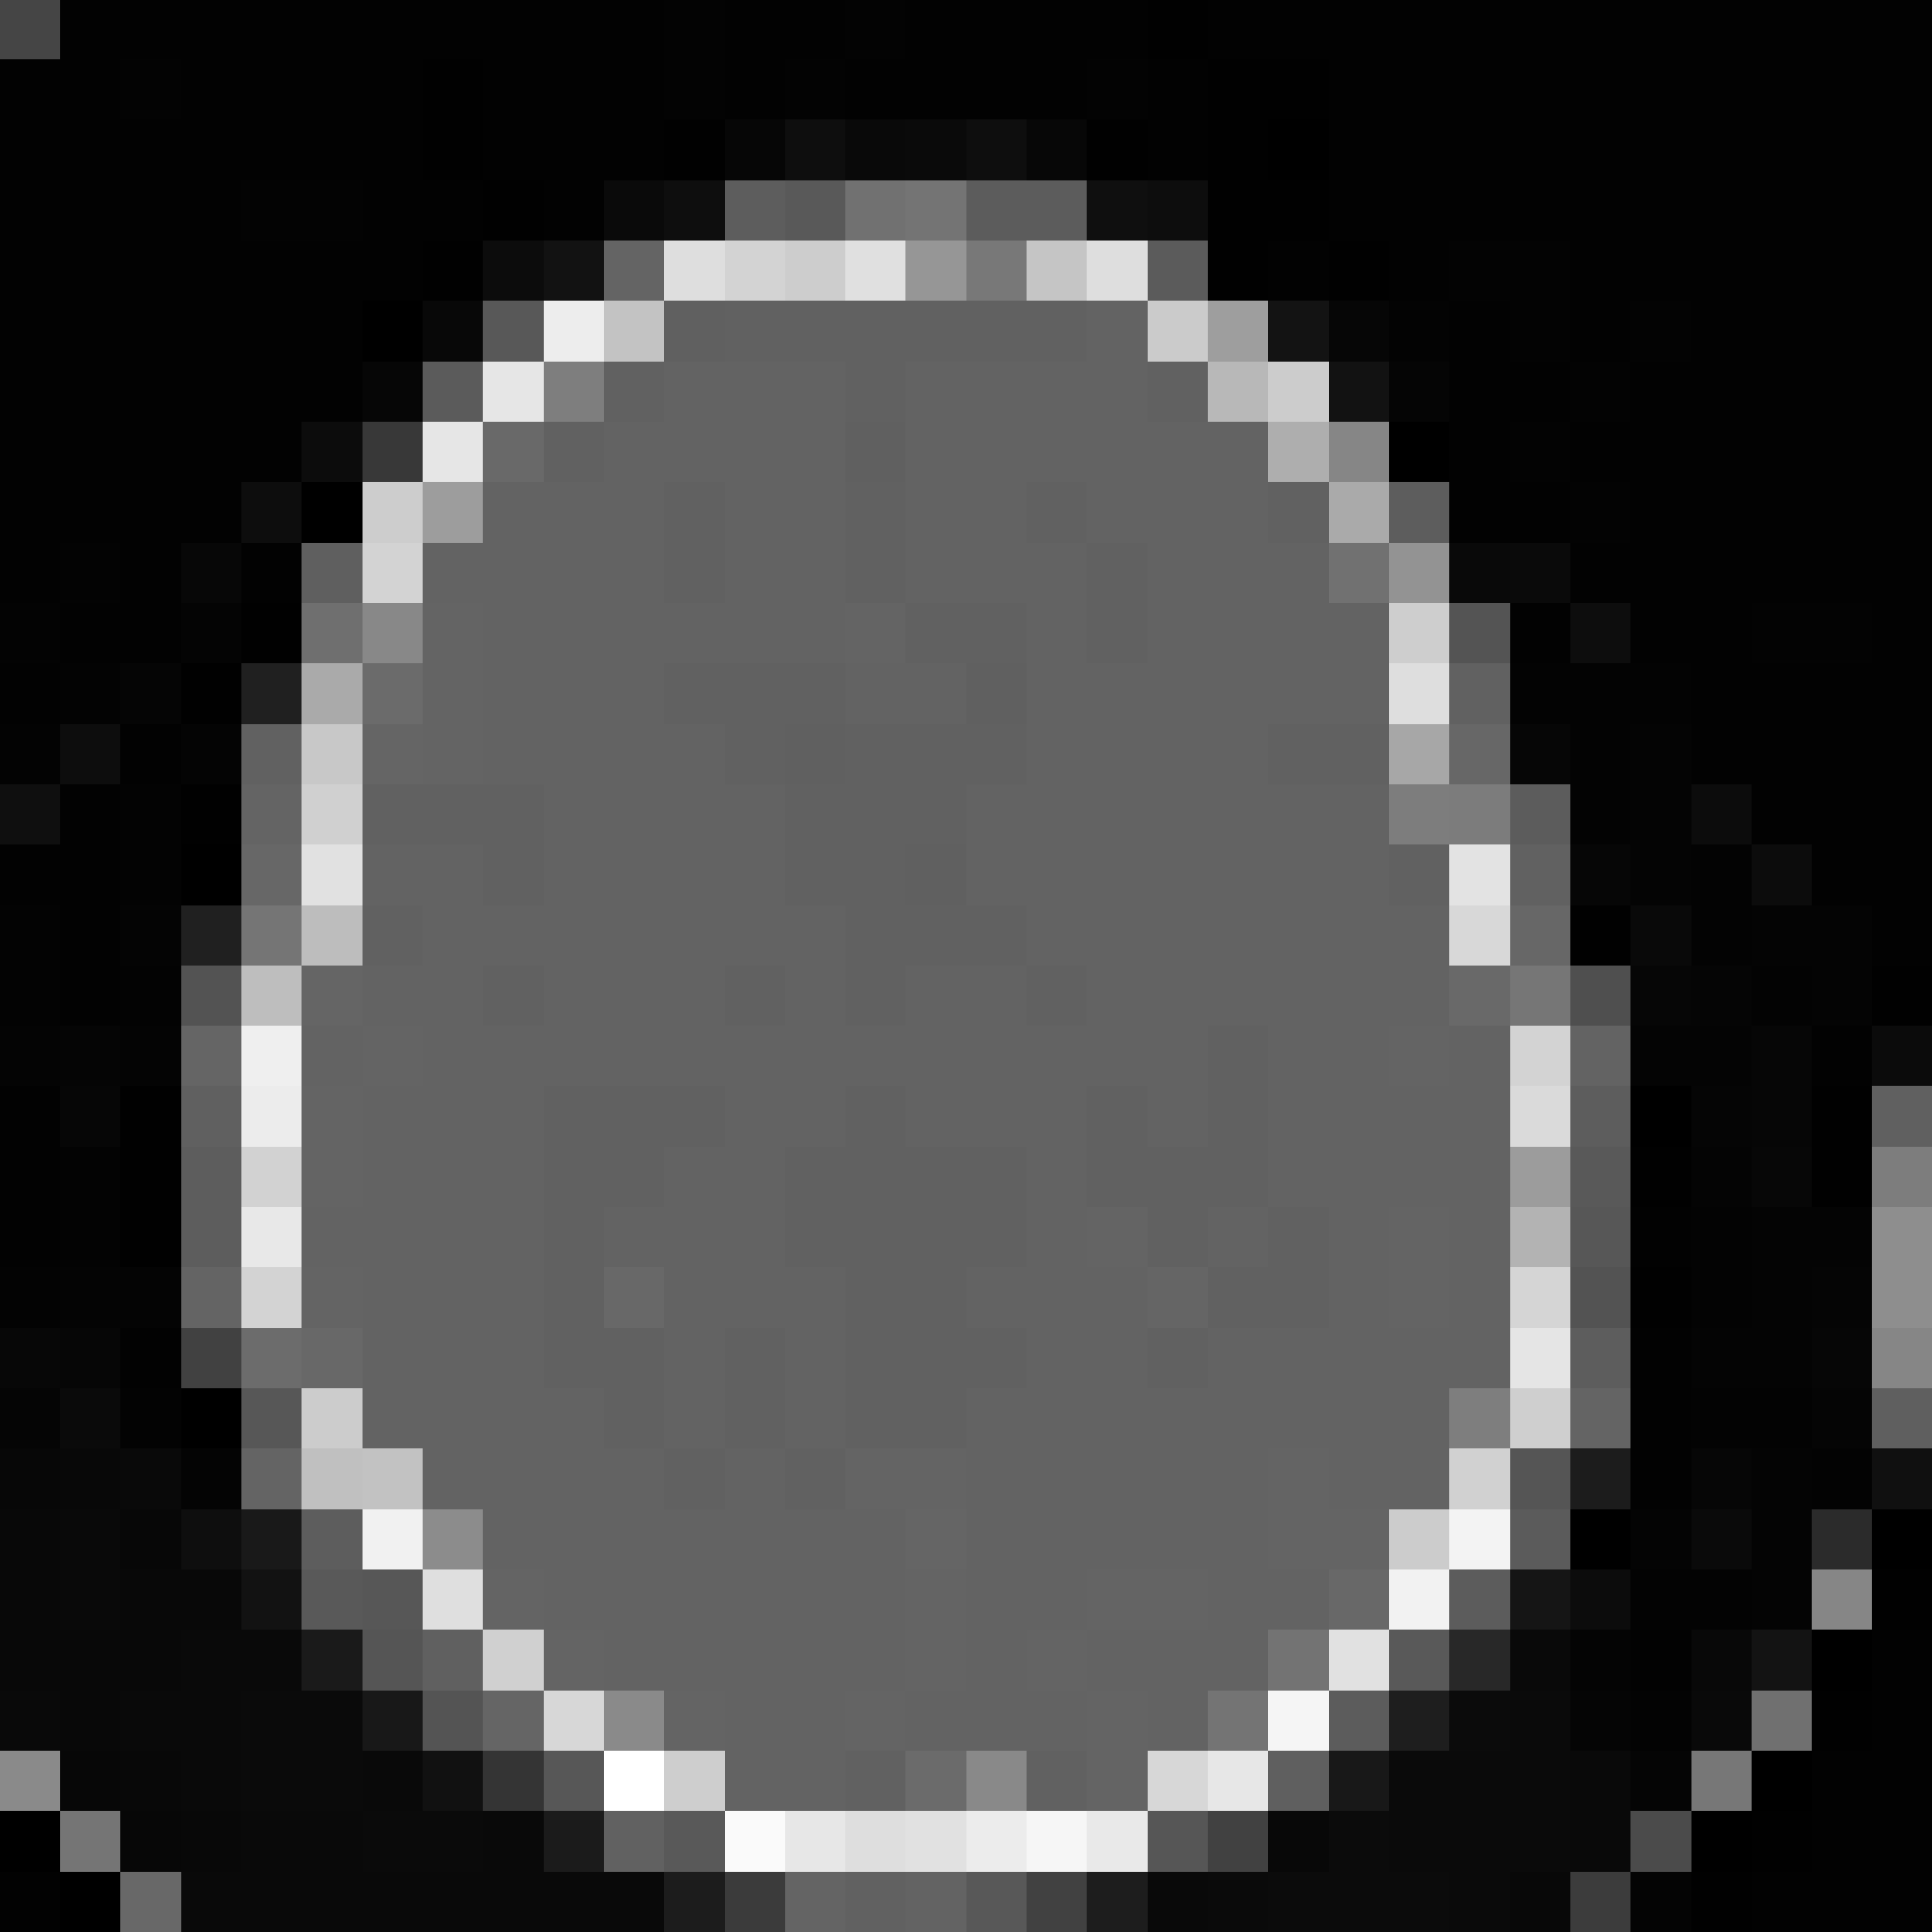
\includegraphics[width=\textwidth]{Figuras/Interpolate_nn_f=0.25.png} 
        \end{subfigure}
        \begin{subfigure}[h]{0.24\linewidth}
            \centering
            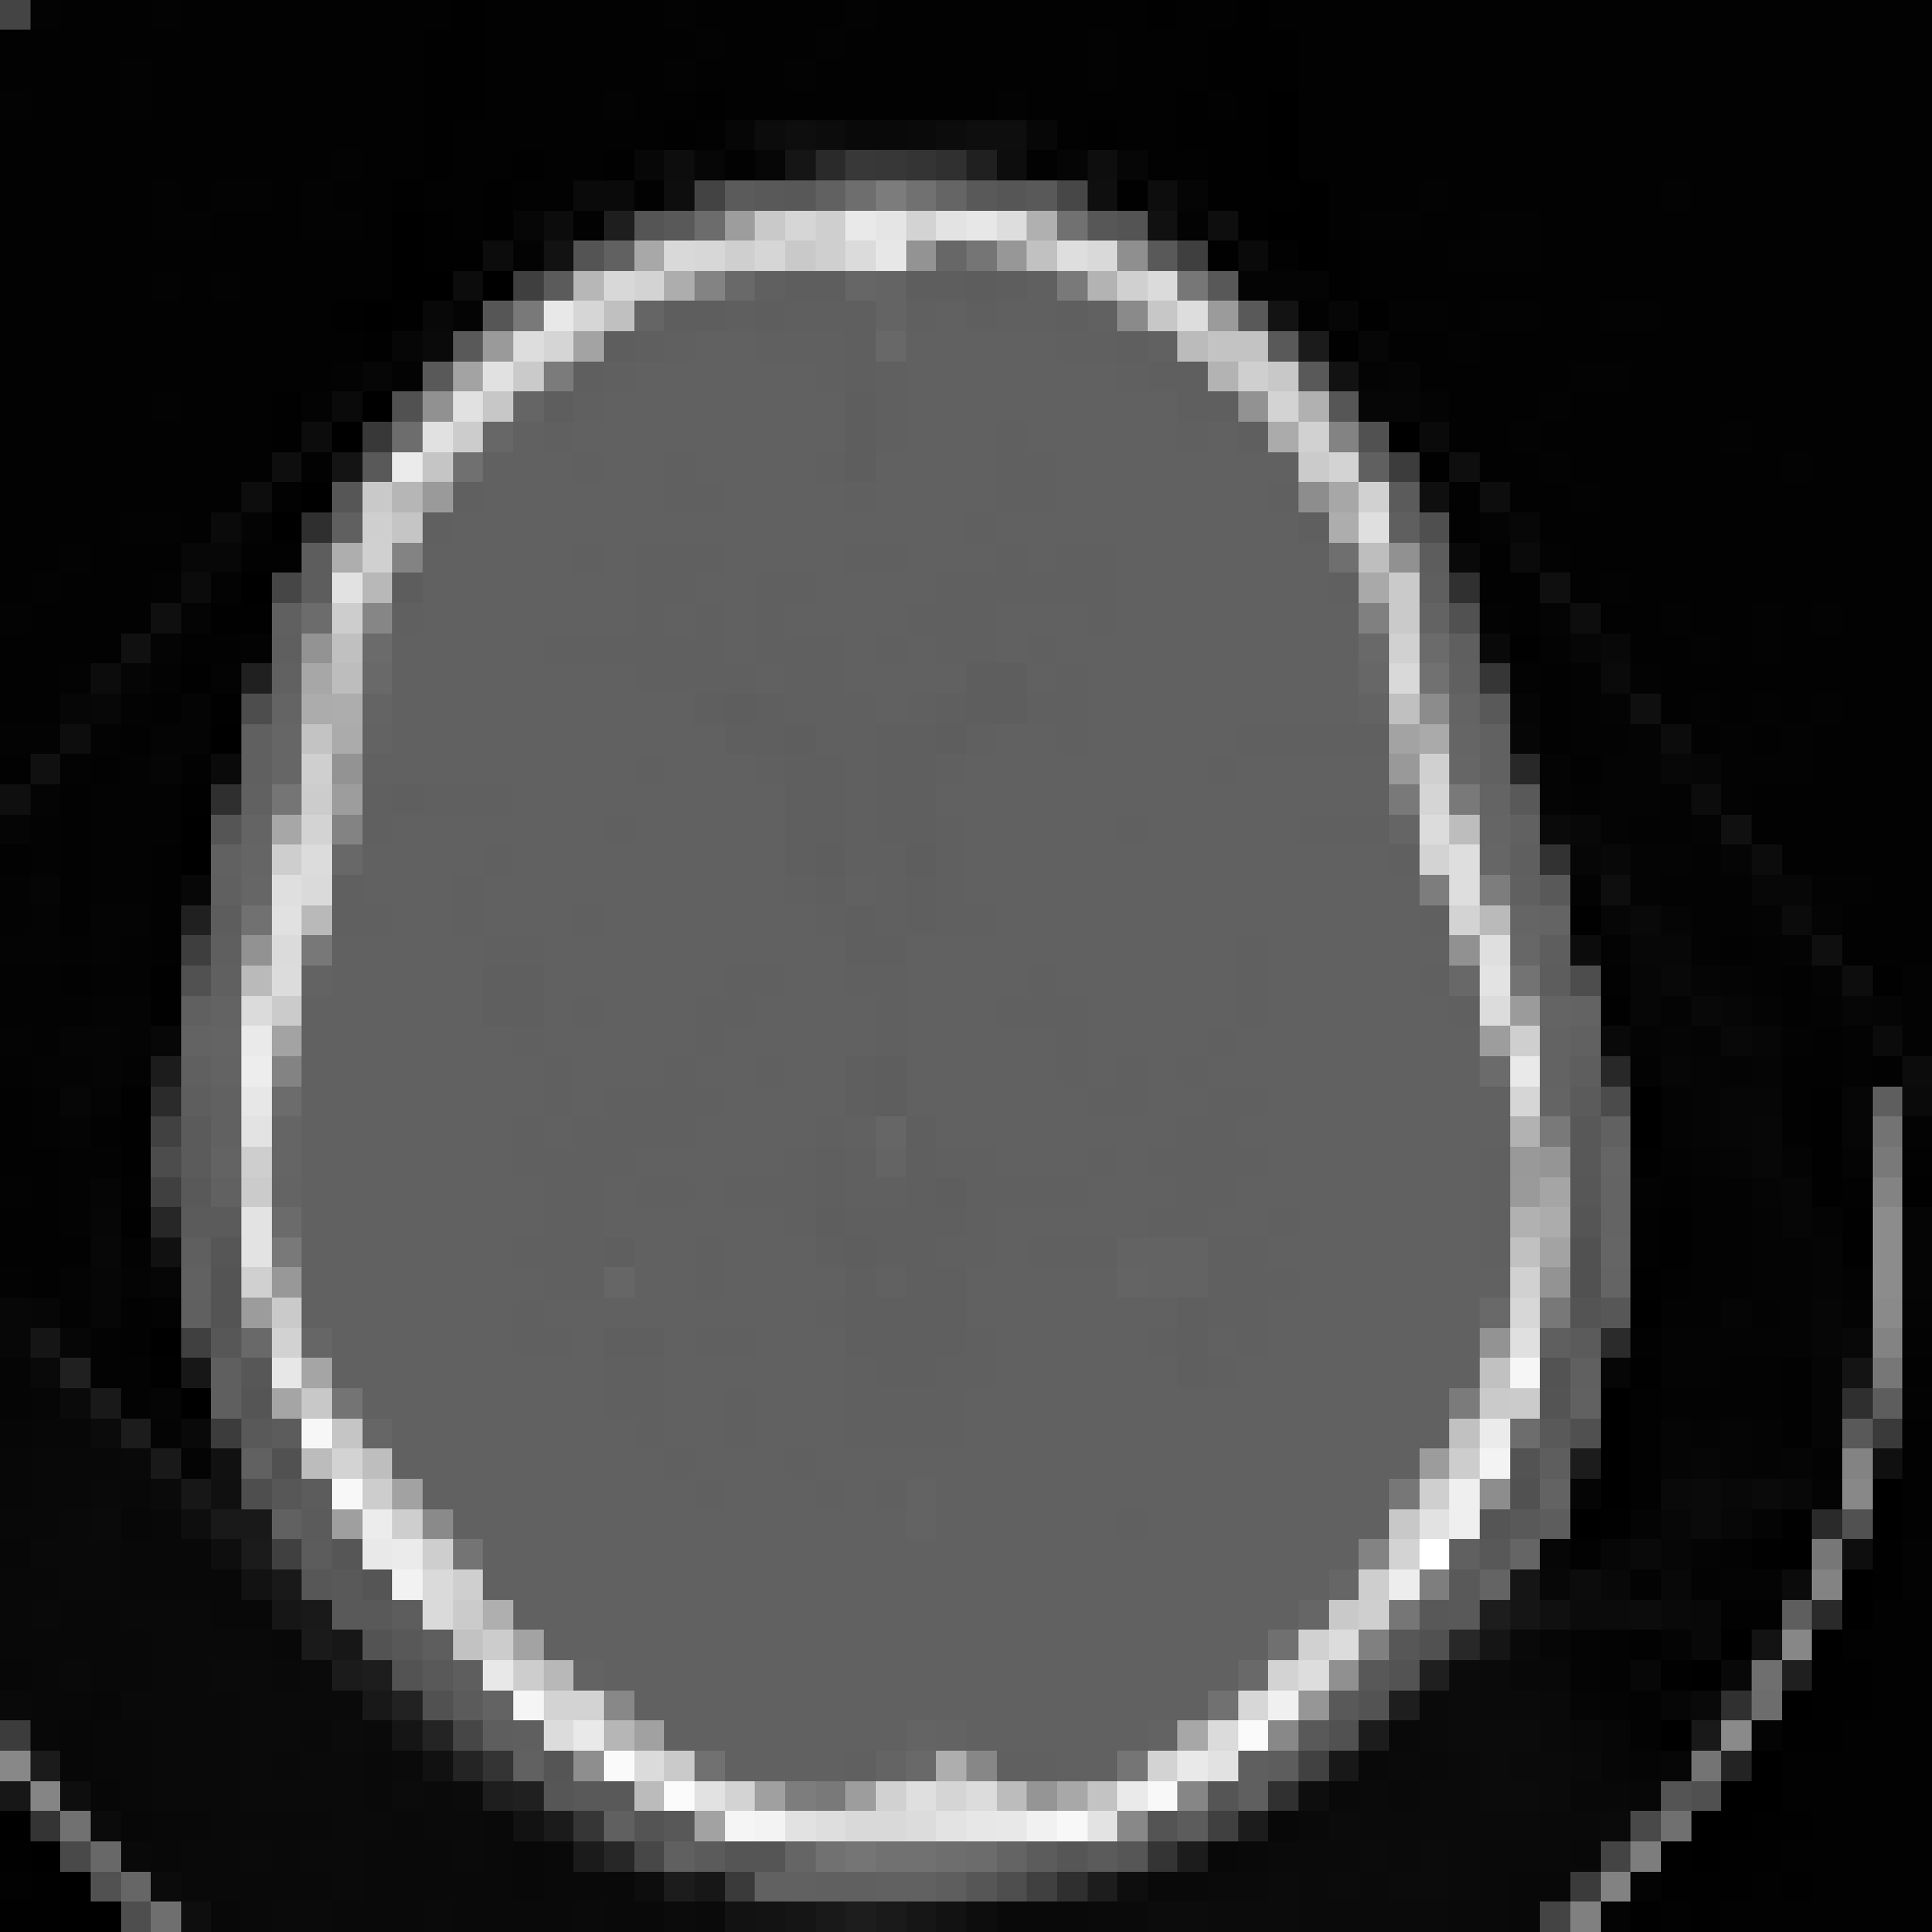
\includegraphics[width=\textwidth]{Figuras/Interpolate_nn_f=0.5.png}
        \end{subfigure}
        \begin{subfigure}[h]{0.24\linewidth}
            \centering
            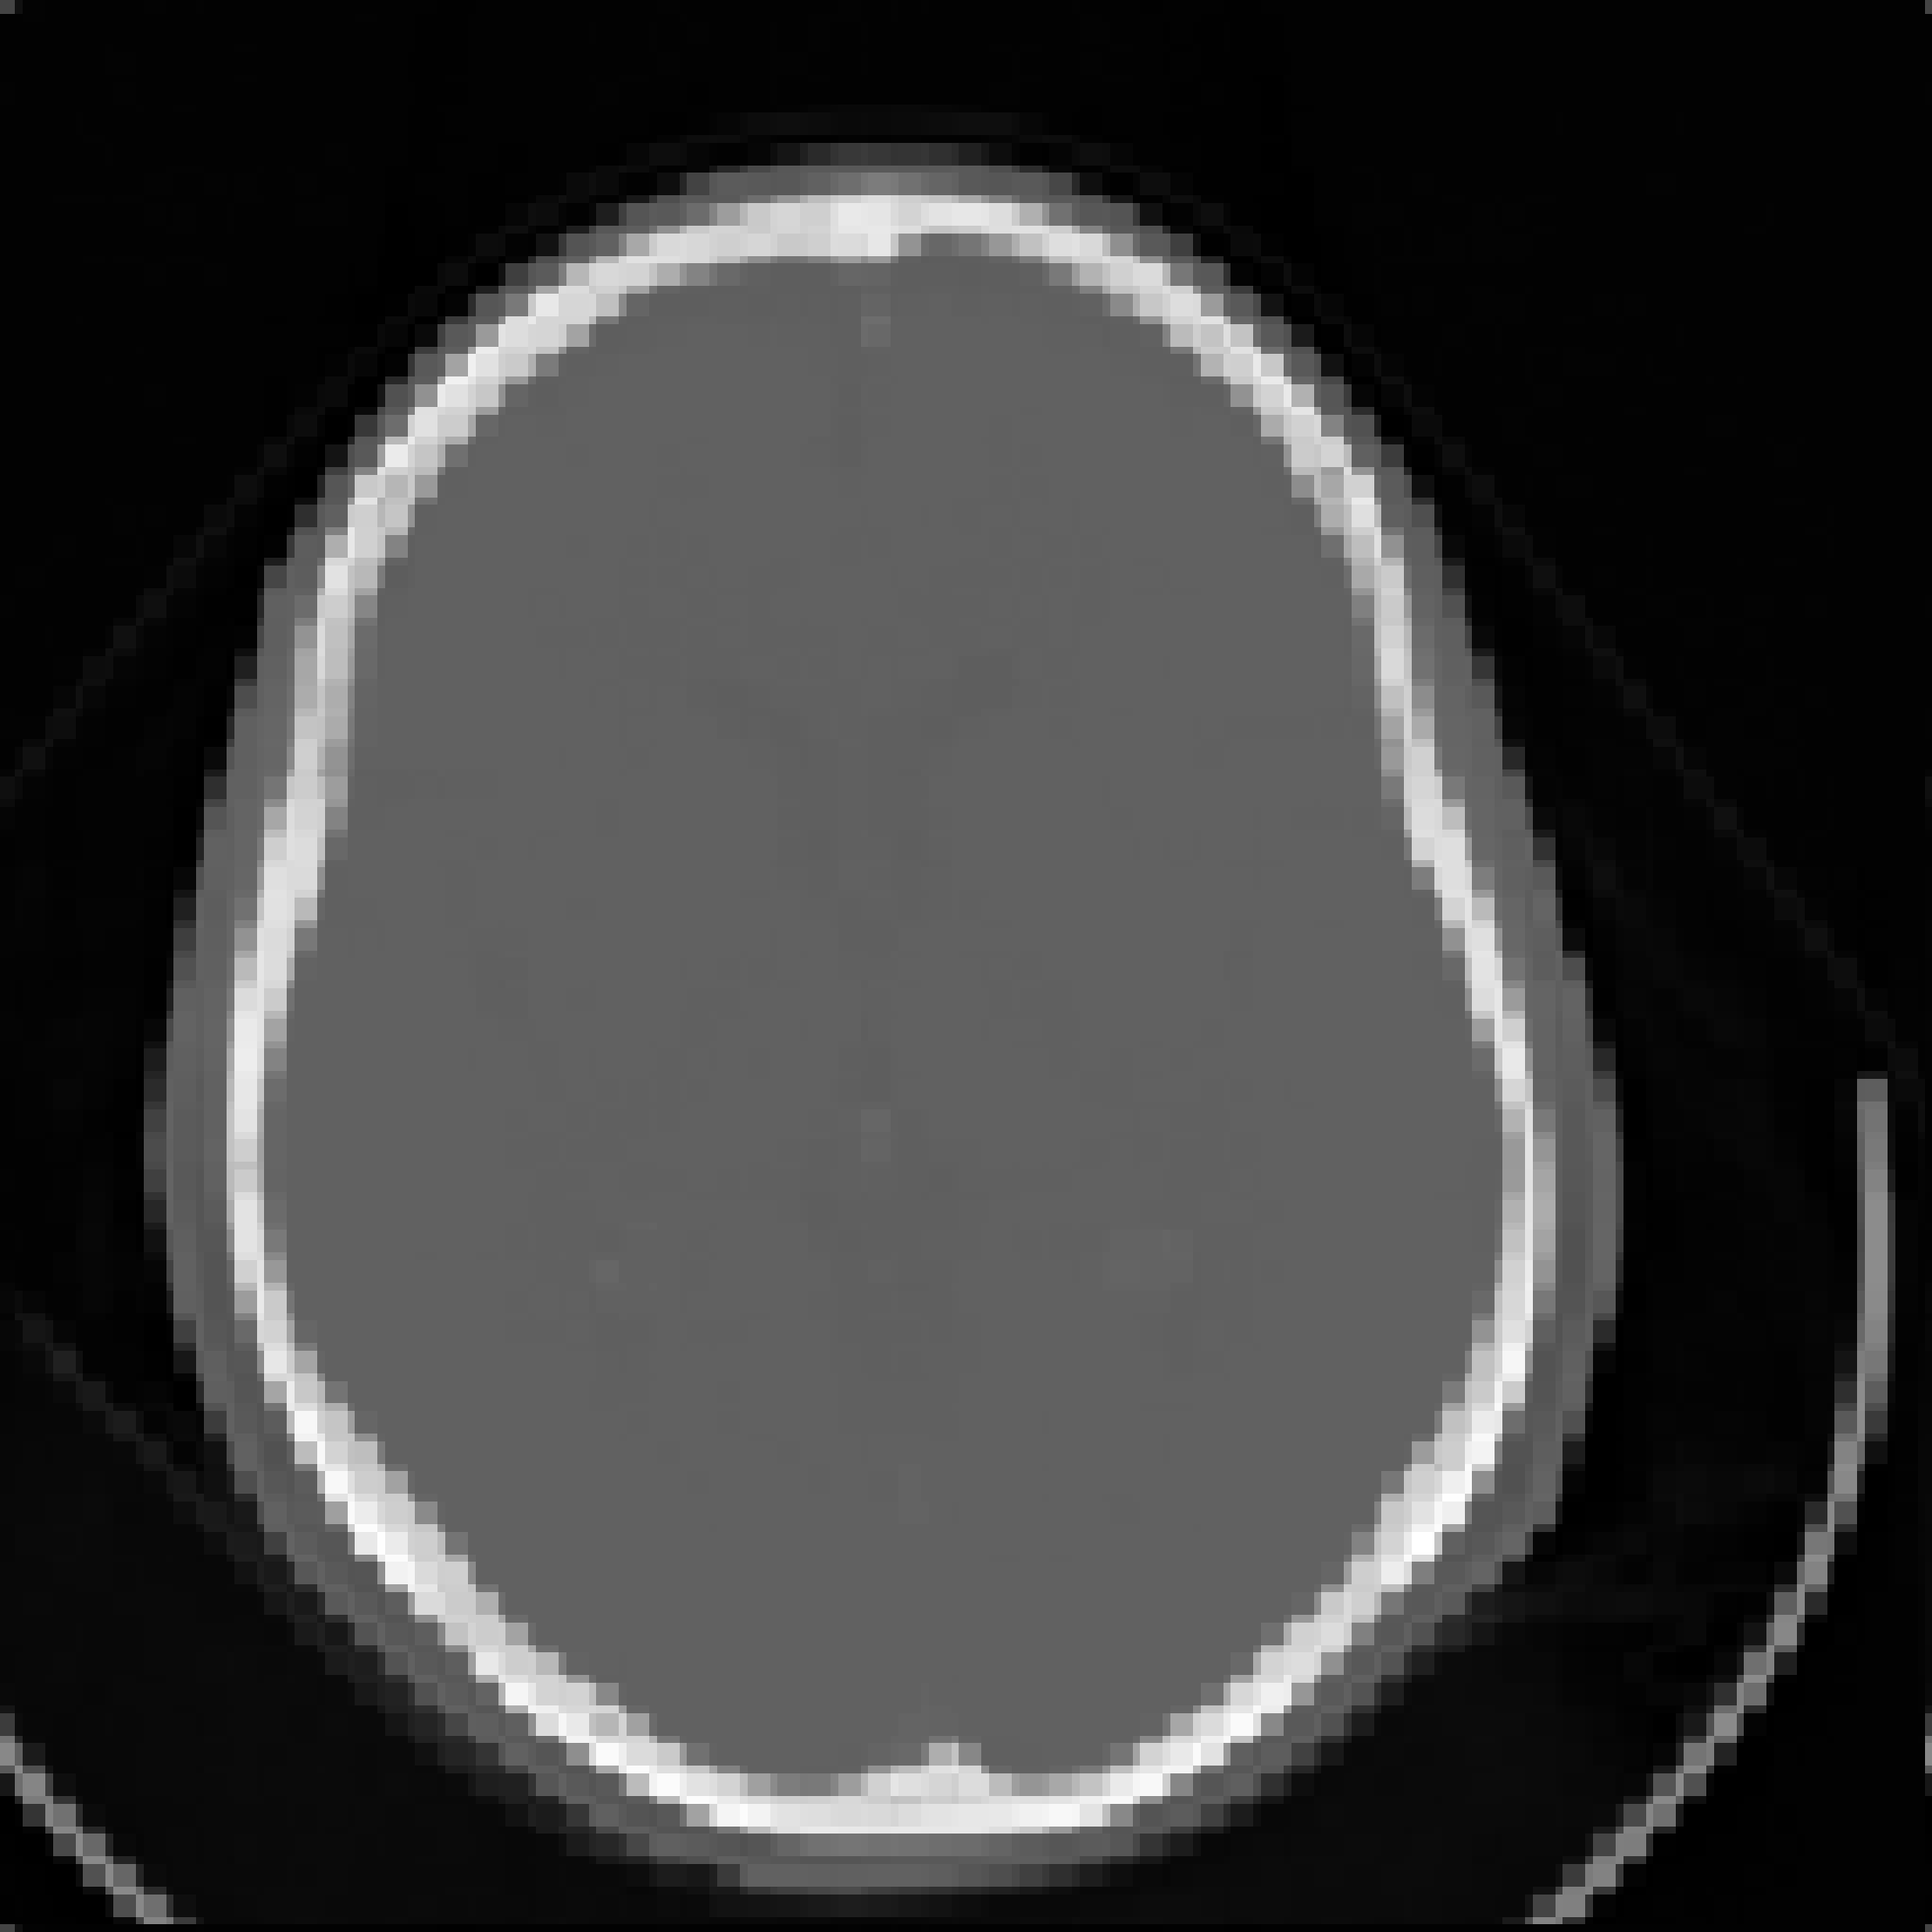
\includegraphics[width=\textwidth]{Figuras/Interpolate_nn_f=2.png}
        \end{subfigure}
        \begin{subfigure}[h]{0.24\linewidth}
            \centering
            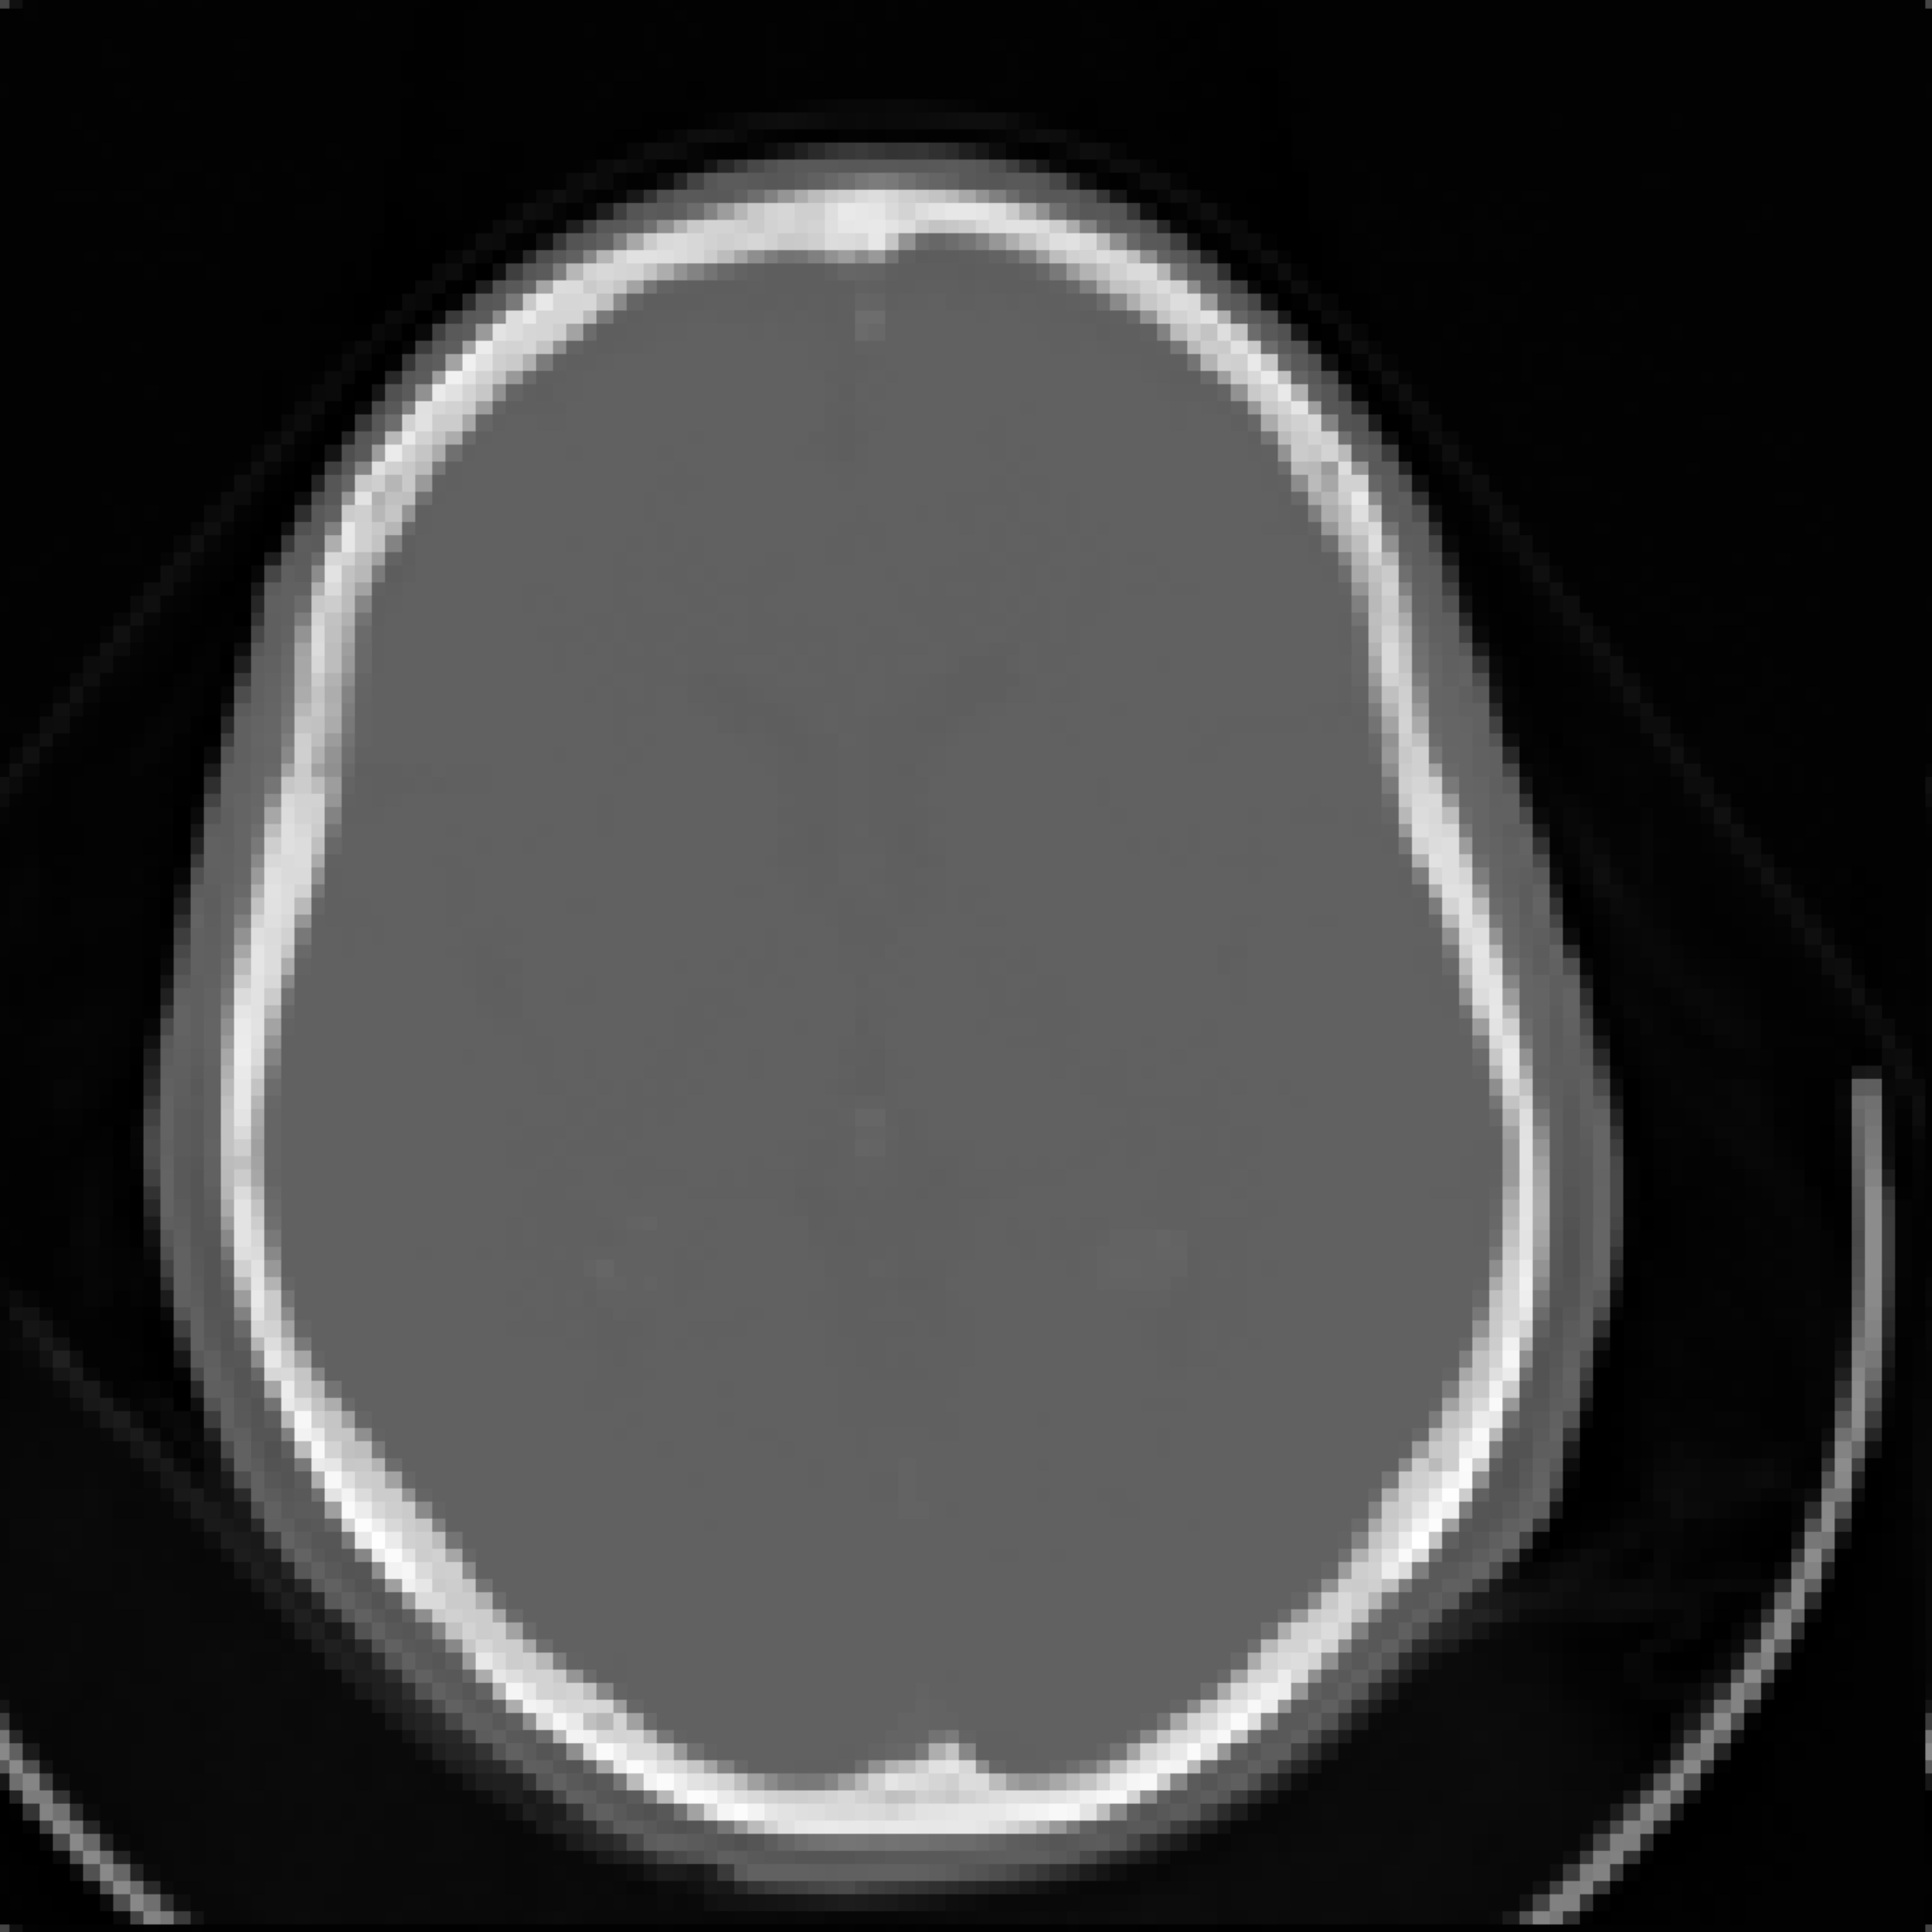
\includegraphics[width=\textwidth]{Figuras/Interpolate_nn_f=8.png}
        \end{subfigure}
         \begin{subfigure}[h]{0.24\linewidth}
            \centering
            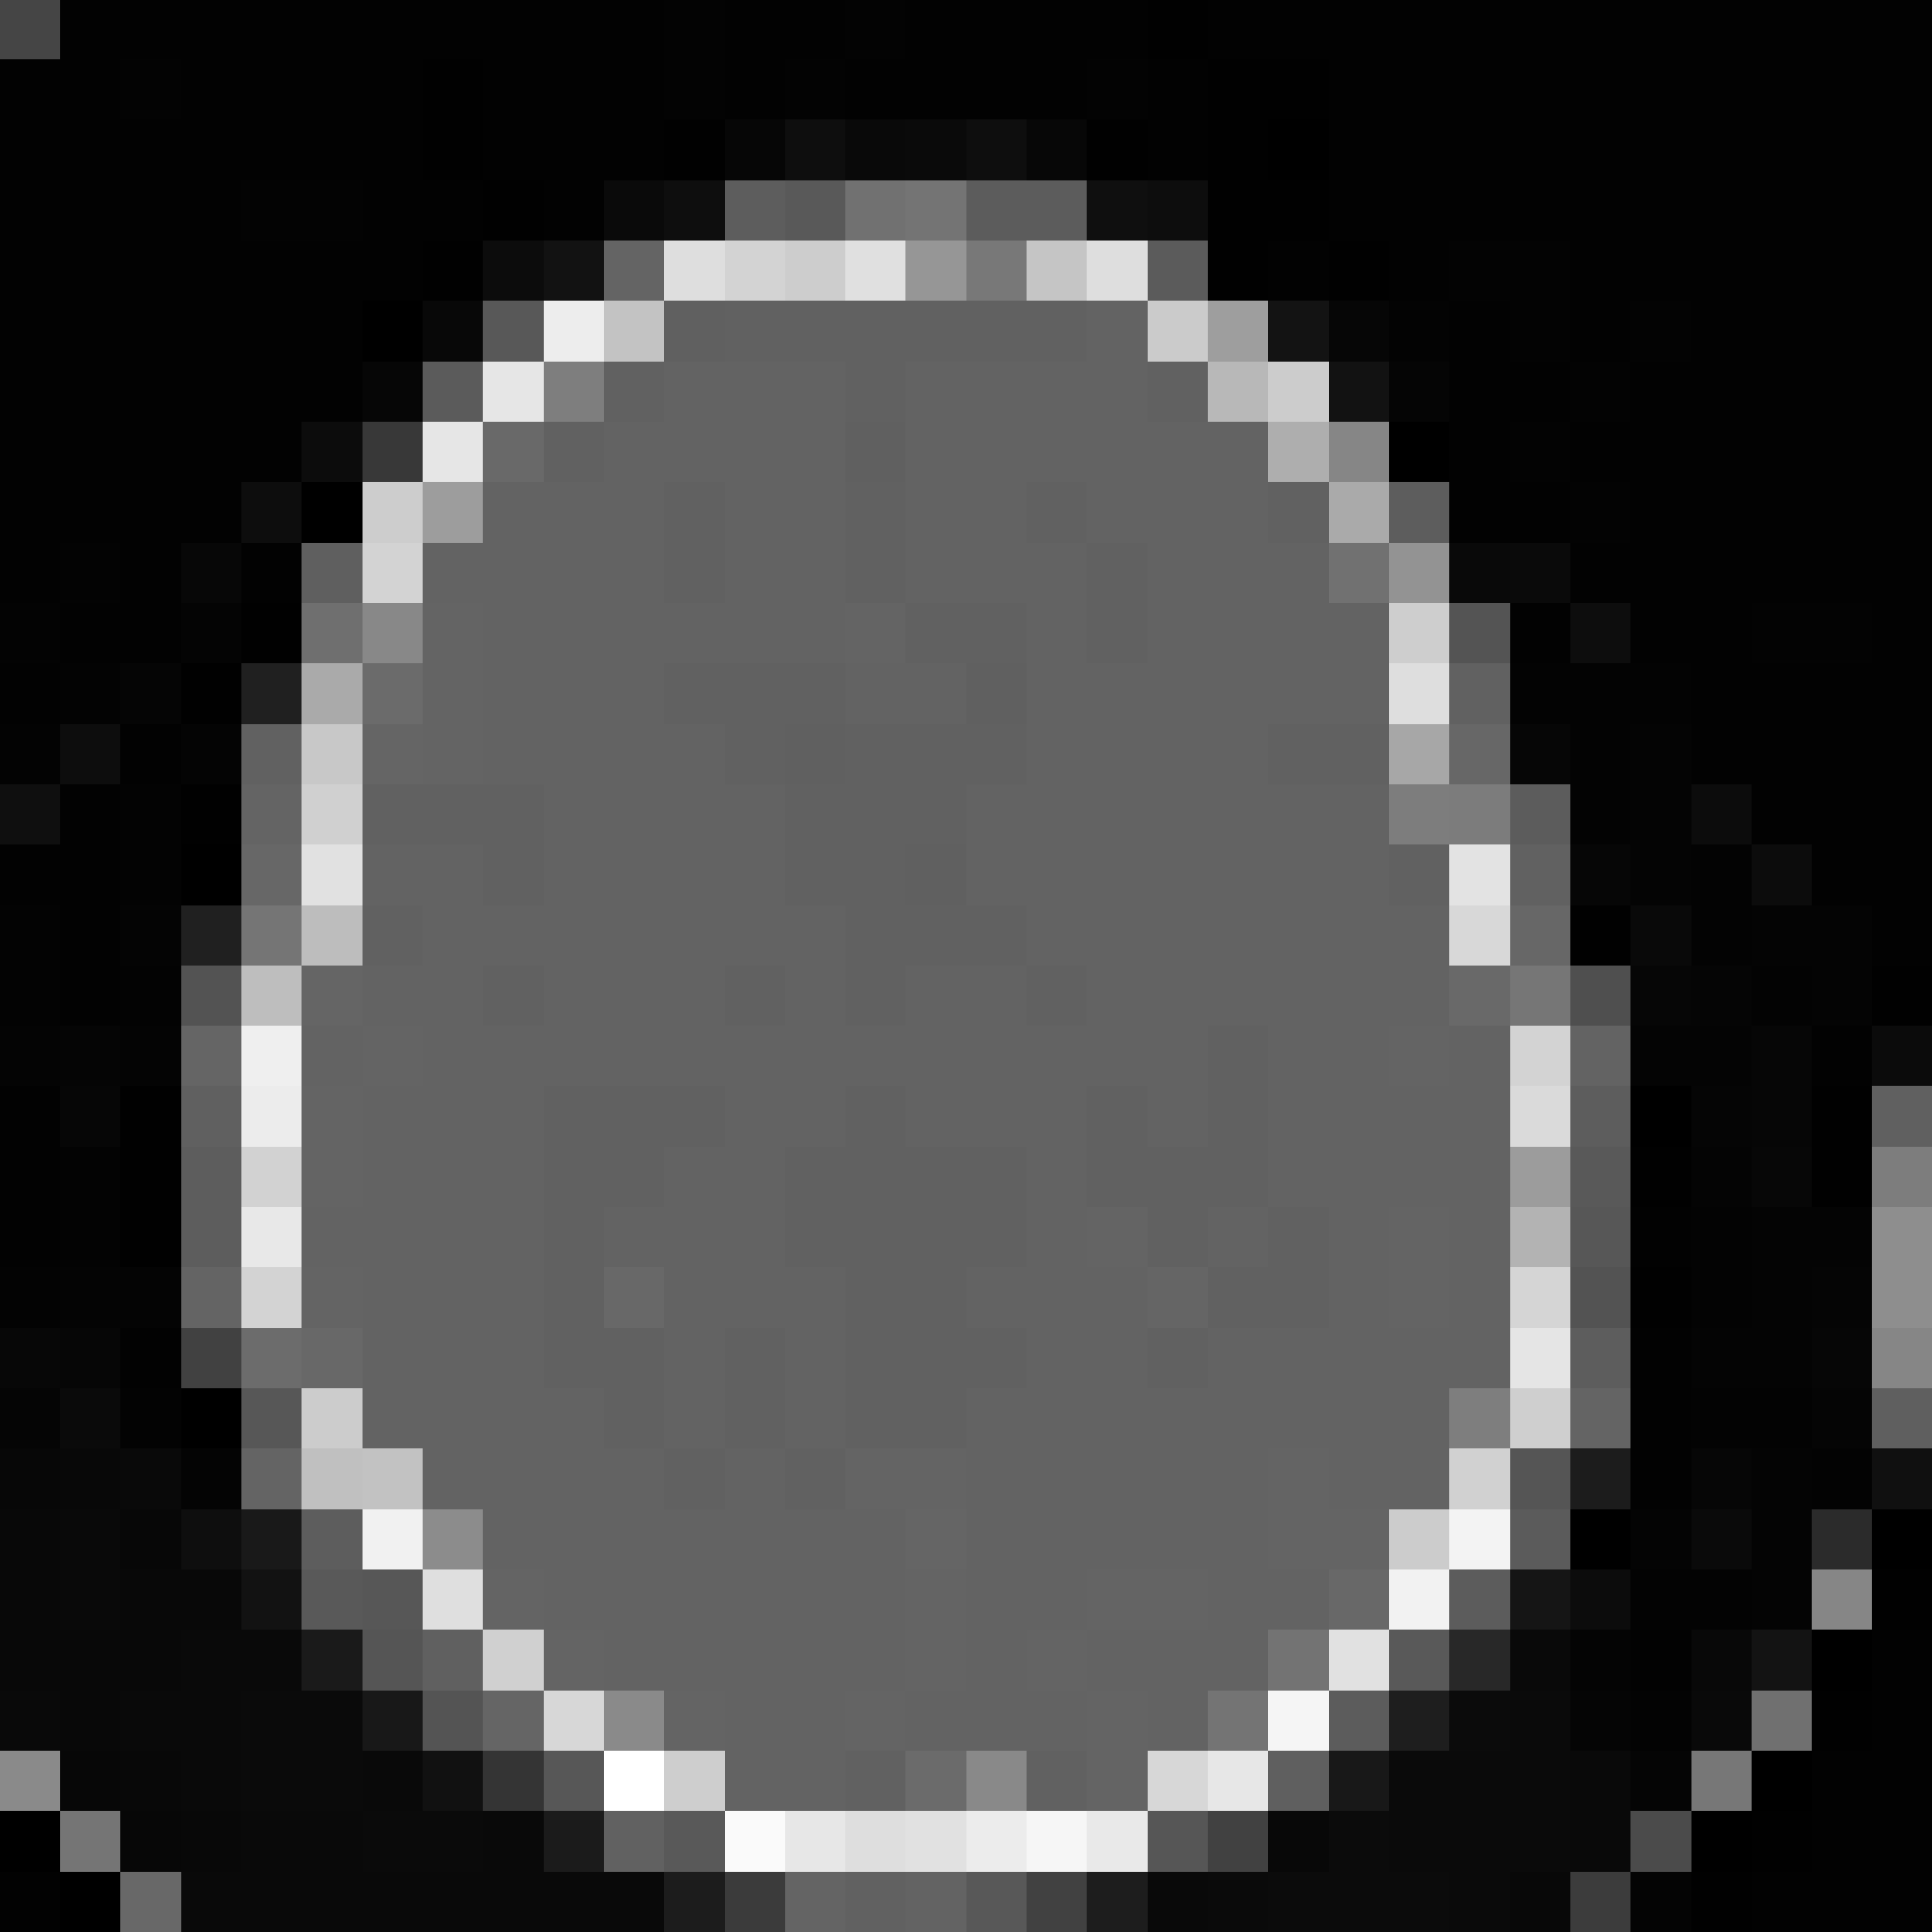
\includegraphics[width=\textwidth]{Figuras/Interpolate_bilinear_f=0.25.png}
            \caption{$32\times32$ \\
            $~$} 
         \end{subfigure}
         \begin{subfigure}[h]{0.24\linewidth}
            \centering
            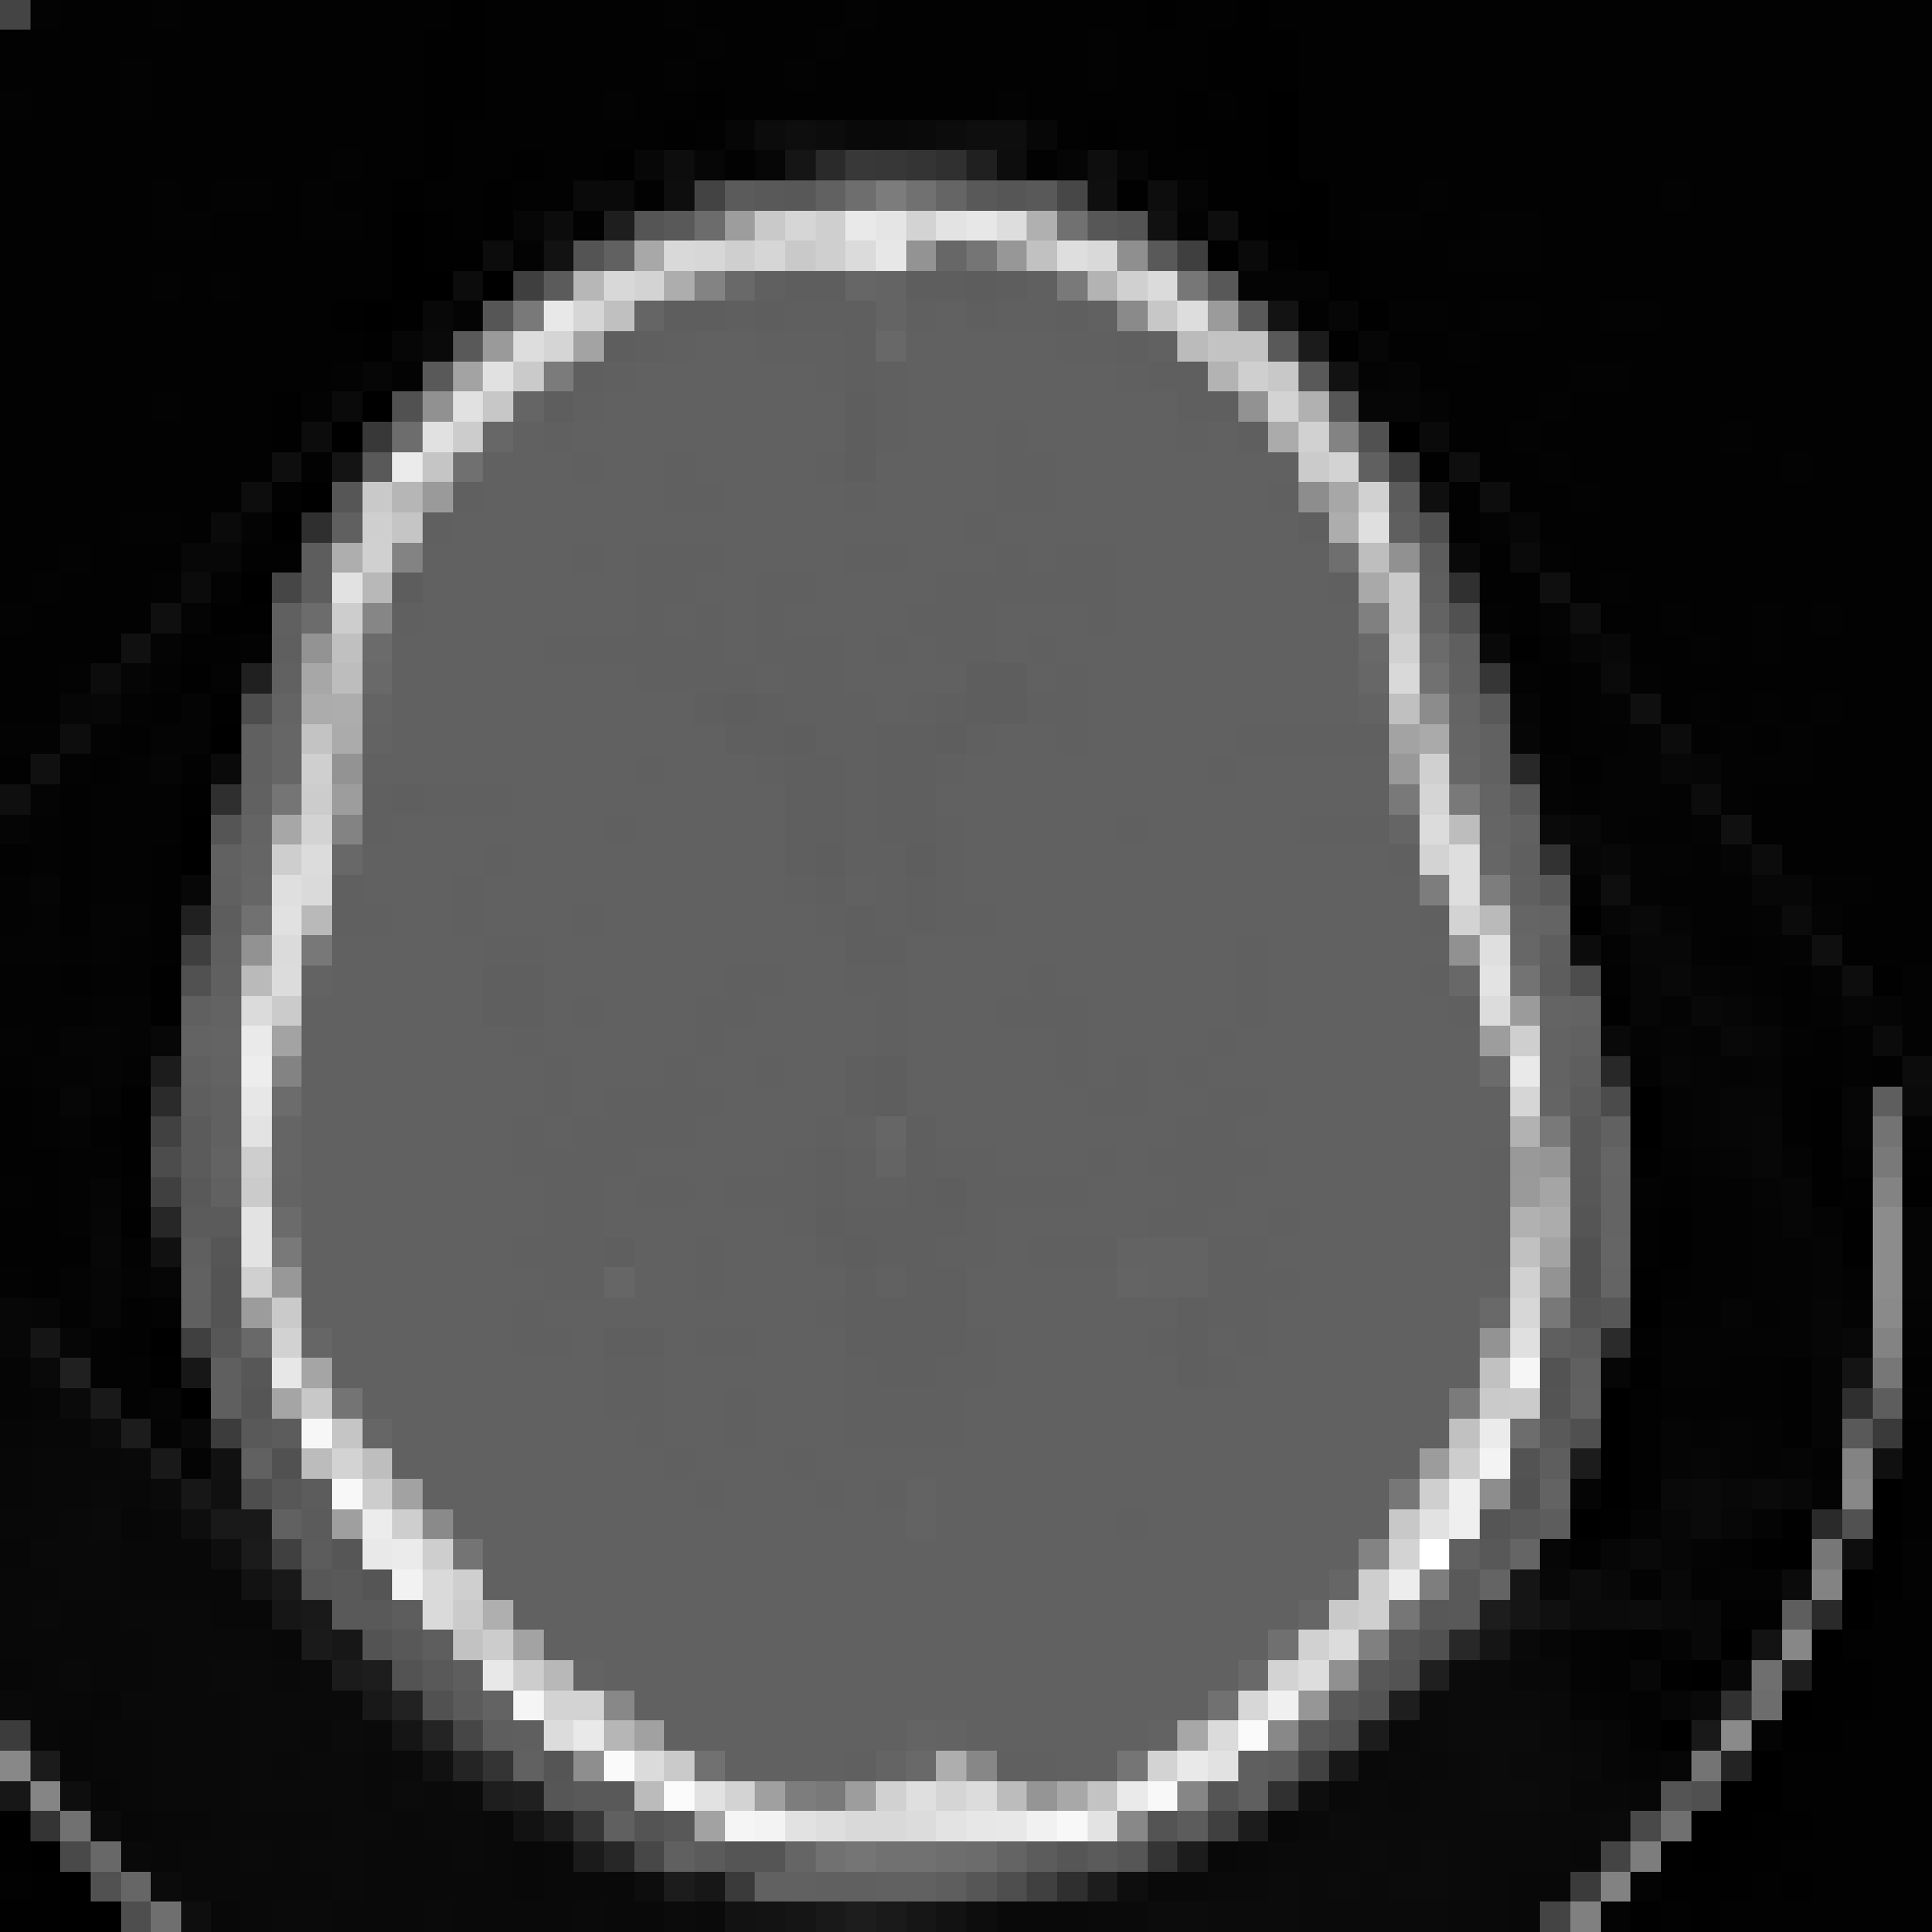
\includegraphics[width=\textwidth]{Figuras/Interpolate_bilinear_f=0.5.png}
            \caption{$64\times64$ \\
            $~$} 
         \end{subfigure}
         \begin{subfigure}[h]{0.24\linewidth}
            \centering
            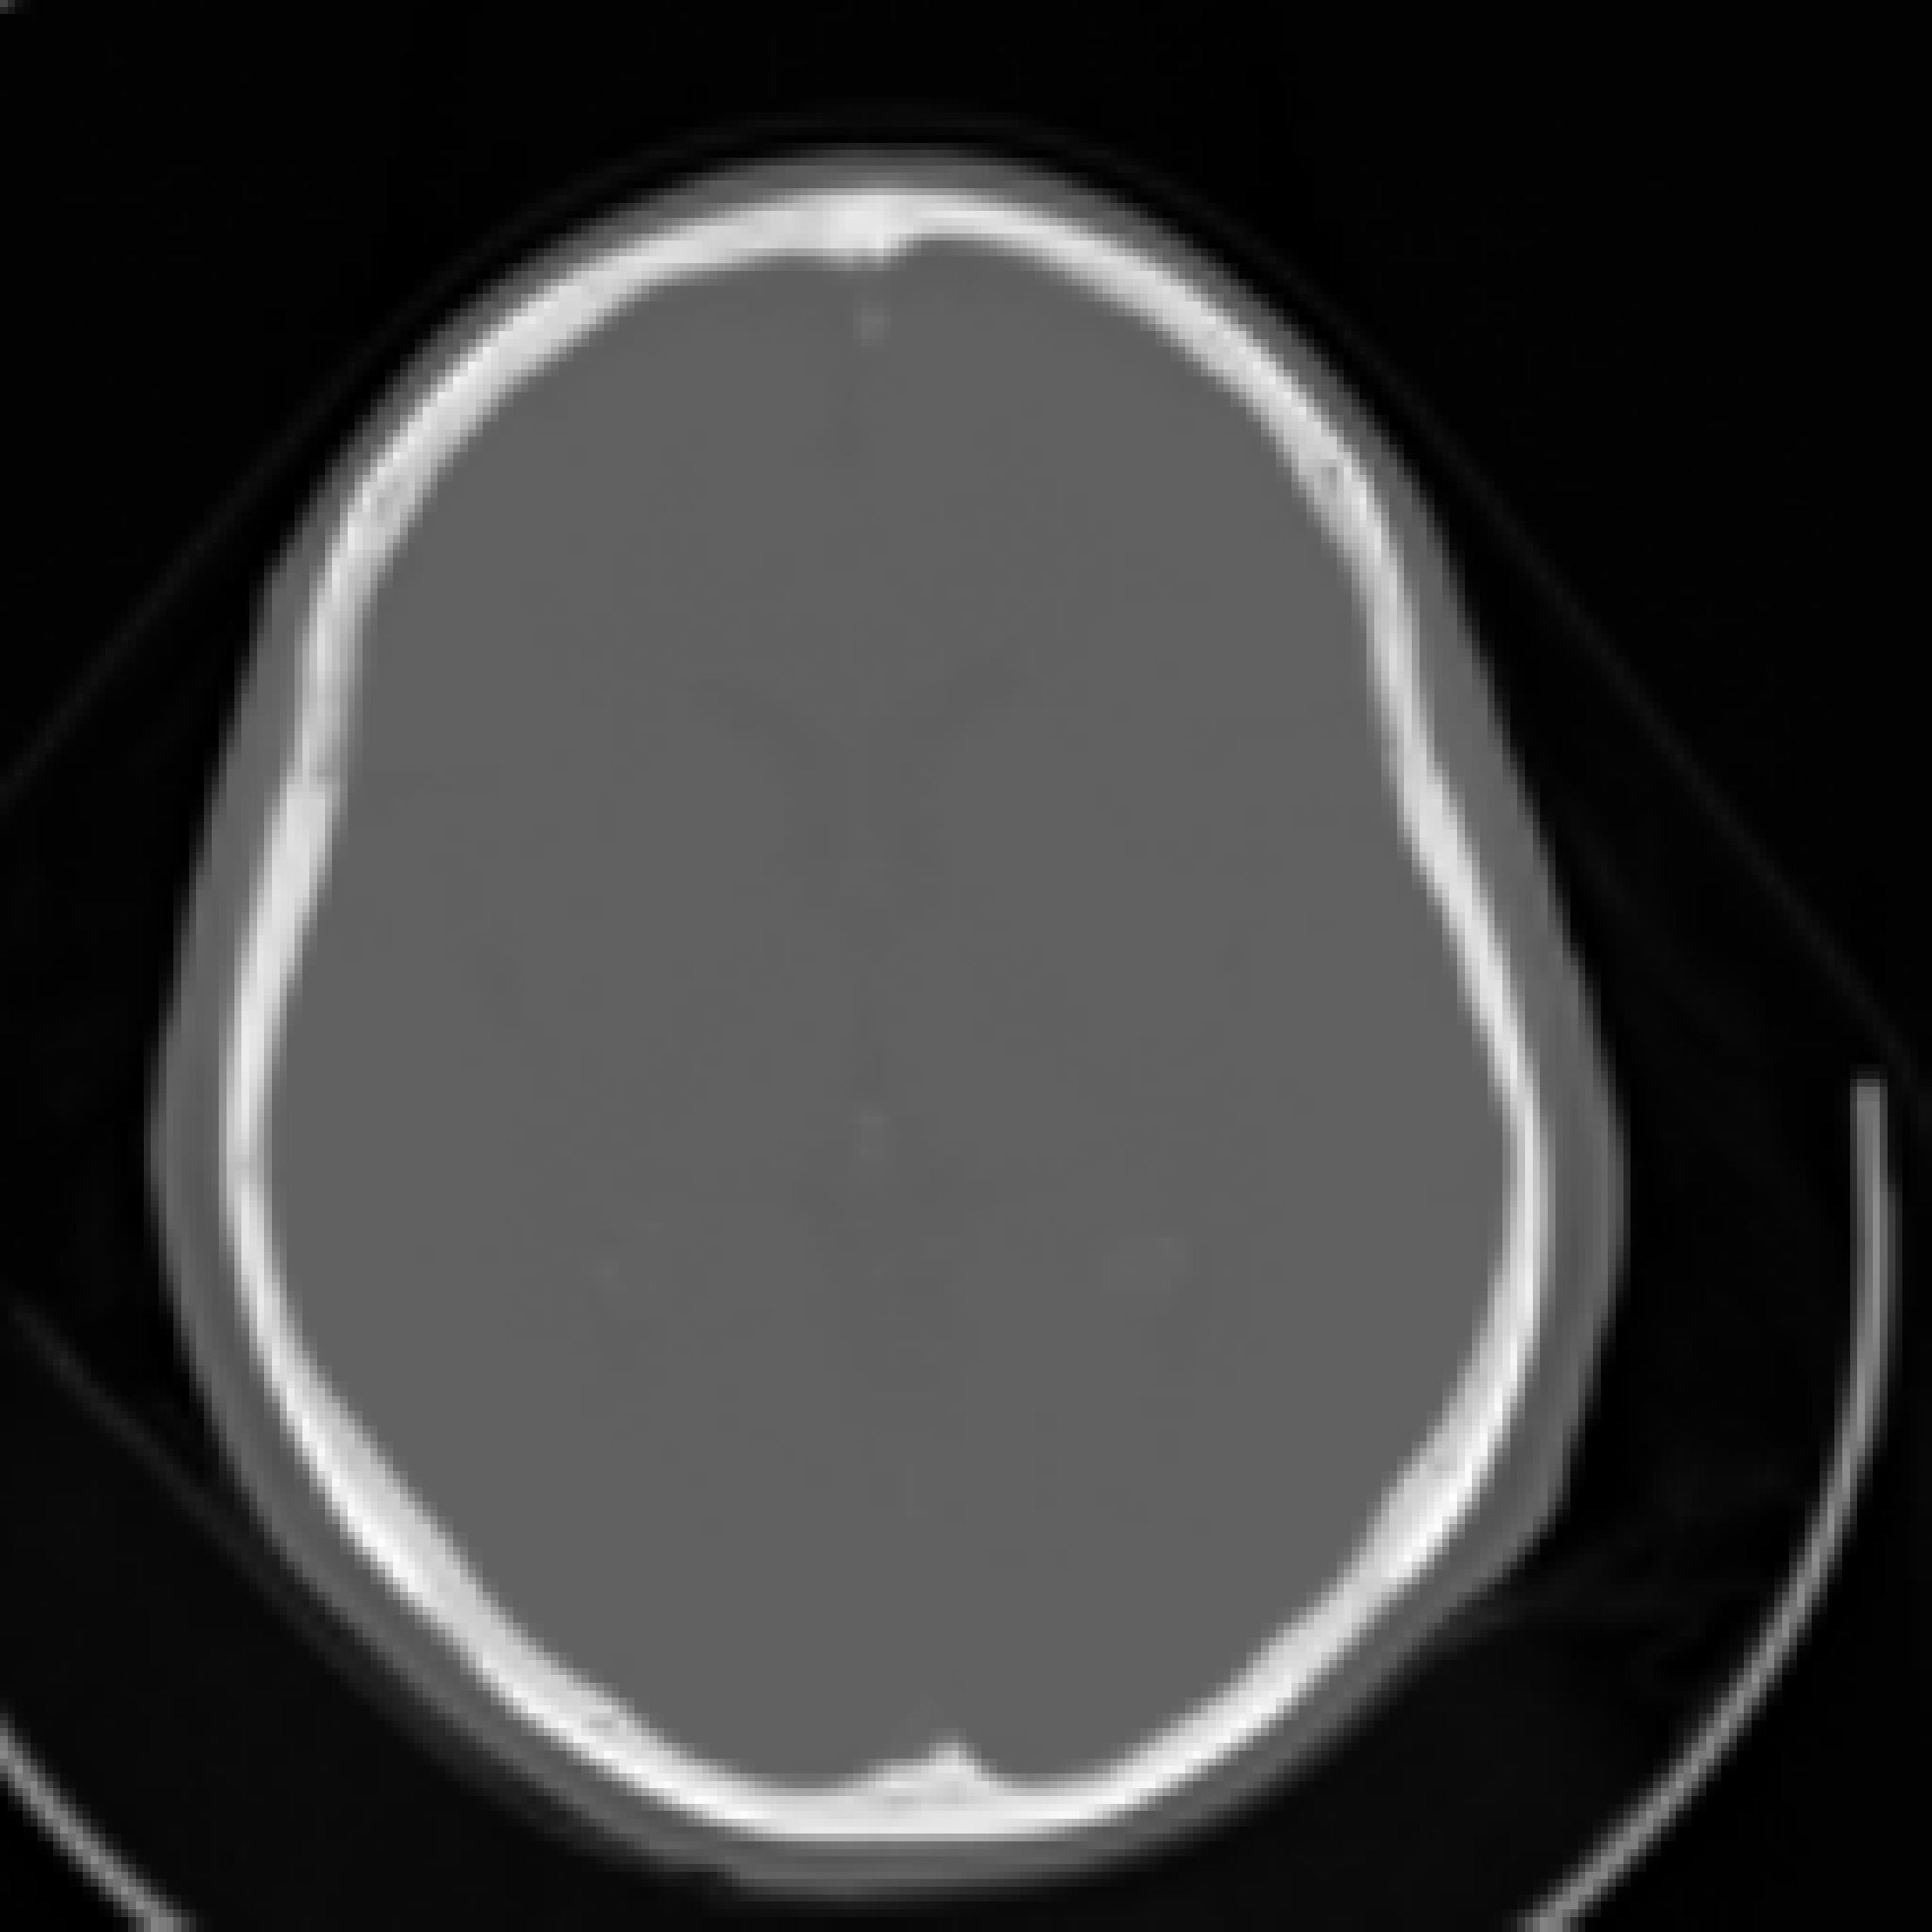
\includegraphics[width=\textwidth]{Figuras/Interpolate_bilinear_f=2.png}
            \caption{$256\times256$ \\
            $~$} 
         \end{subfigure}
         \begin{subfigure}[h]{0.24\linewidth}
            \centering
            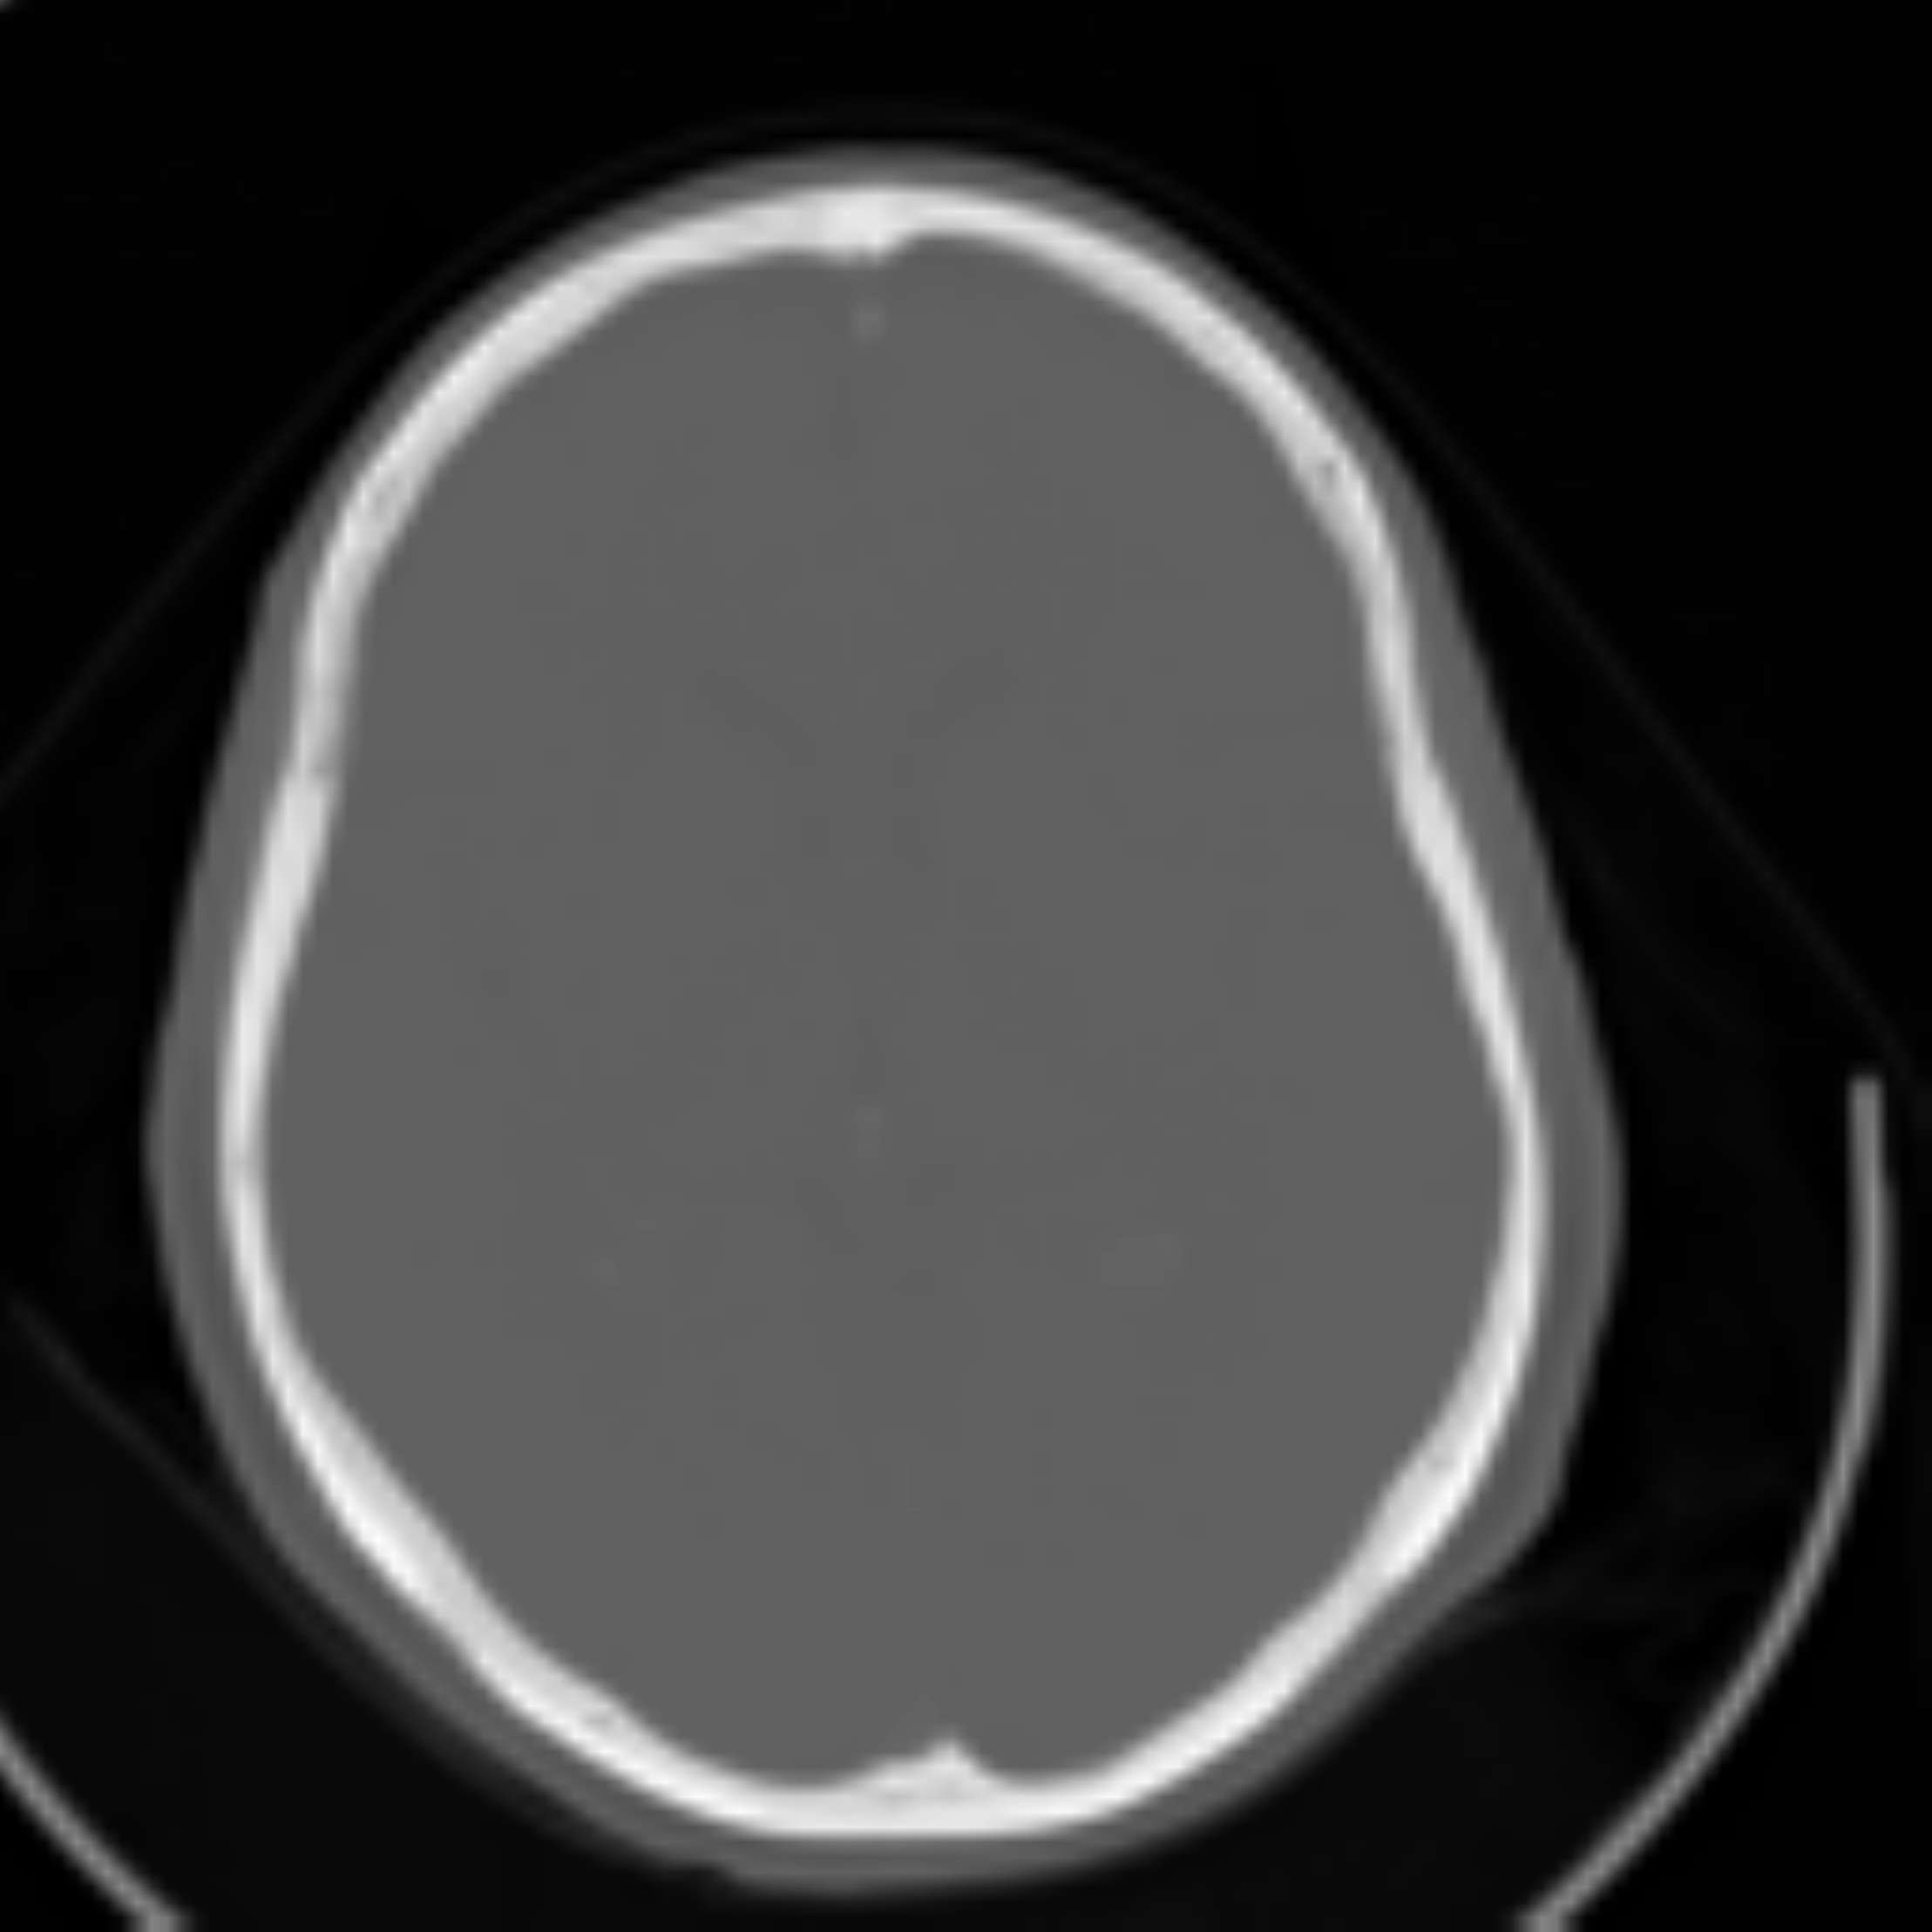
\includegraphics[width=\textwidth]{Figuras/Interpolate_bilinear_f=8.png}
            \caption{$1024\times1024$} 
         \end{subfigure}
    \caption{Distintos reescaleos de la imagenC con interpolación por los métodos de vecinos más cercanos (arriba) y bilineal (abajo).}
    \label{fig:Interpolate}
\end{figure}

\section{Filtros en el dominio espacial\label{sec:ej4}}

\vspace{0.3cm}

Se aplicaron filtros promedios pasabajos a las imágenes A y C con kernels de $3\times3$, $5\times5$ y $7\times7$ como se muestra en la Fig. \ref{fig:Pasabajo} utilizando ImageJ. Estos filtros se definen a partir de kernels de la forma 
\begin{equation}
    h = \frac{1}{n^2} 
    \begin{bmatrix}
    1 & \cdots & 1 \\
    \vdots & \ddots & \vdots \\
    1 & \cdots & 1 \\
    \end{bmatrix}
\end{equation}
donde $n$ es la dimensión de la matriz. 

Se observa que a medida que se aumenta la dimensión del kernel, la imagen se vuelve cada vez más borrosa, es decir, el suavizado es mayor.

\begin{figure}[h]
    \centering
         \begin{subfigure}[h]{0.24\linewidth}
            \centering
            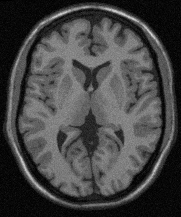
\includegraphics[width=\textwidth]{Figuras/ImagenA.png}
            \caption{Original} 
         \end{subfigure}
         \begin{subfigure}[h]{0.24\linewidth}
            \centering
            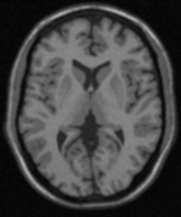
\includegraphics[width=\textwidth]{Figuras/ImagenA3x3.png}
            \caption{\centering $3\times3$} 
         \end{subfigure}
         \begin{subfigure}[h]{0.24\linewidth}
            \centering
            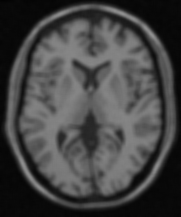
\includegraphics[width=\textwidth]{Figuras/ImagenA5x5.png}
            \caption{$5\times5$} 
         \end{subfigure}
         \begin{subfigure}[h]{0.24\linewidth}
            \centering
            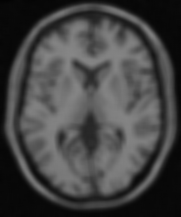
\includegraphics[width=\textwidth]{Figuras/ImagenA7x7.png}
            \caption{$7\times7$} 
         \end{subfigure}
         \begin{subfigure}[h]{0.24\linewidth}
            \centering
            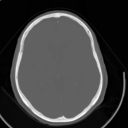
\includegraphics[width=\textwidth]{Figuras/ImagenC.png}
            \caption{Original} 
         \end{subfigure}
         \begin{subfigure}[h]{0.24\linewidth}
            \centering
            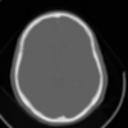
\includegraphics[width=\textwidth]{Figuras/ImagenC3x3.png}
            \caption{$3\times3$} 
         \end{subfigure}
         \begin{subfigure}[h]{0.24\linewidth}
            \centering
            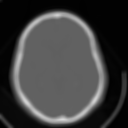
\includegraphics[width=\textwidth]{Figuras/ImagenC5x5.png}
            \caption{$5\times5$} 
         \end{subfigure}
         \begin{subfigure}[h]{0.24\linewidth}
            \centering
            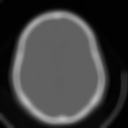
\includegraphics[width=\textwidth]{Figuras/ImagenC7x7.png}
            \caption{$7\times7$} 
         \end{subfigure}
    \caption{Filtros promedios pasabajos aplicados a la imagenA (arriba) y a la imagenC (abajo) para distintas dimensiones de kernels.}
    \label{fig:Pasabajo}
\end{figure}


\section{Filtros en el dominio de frecuencias\label{sec:ej5}}

\vspace{0.3cm}

Dada una figura con componentes periodicas en su textura como la que se muestra en la Fig. \ref{fig:superman}a es posible eliminar dichas componentes a partir de un procesamiento en el espacio de frecuencias de dicha imagen. Para esto se calcula la transformada de Fourier rápida (FFT por sus siglas en inglés) de la imagen con ImageJ y luego de reconocer las componentes periodicas, que en el espacio de frecuencias se manifiestan como puntos de alta intensidad, se procede a eliminarlas. Una vez eliminadas estas componentes se antitransforma la imagen (inverse FFT) y se recupera la imagen original con las componentes periodicas eliminadas. En la Fig. \ref{fig:superman} se muestra la imagen original (a) y la imagen procesada (b), mientras que en la Fig. \ref{fig:supermanfft} se muestra el espacio de frecuencias con la transformada de Fourier de la imagen original (a) y la transformada de Fourier con las componentes periodicas eliminadas (b). 

\begin{figure}[h]
    \centering
         \begin{subfigure}[h]{0.49\linewidth}
            \centering
            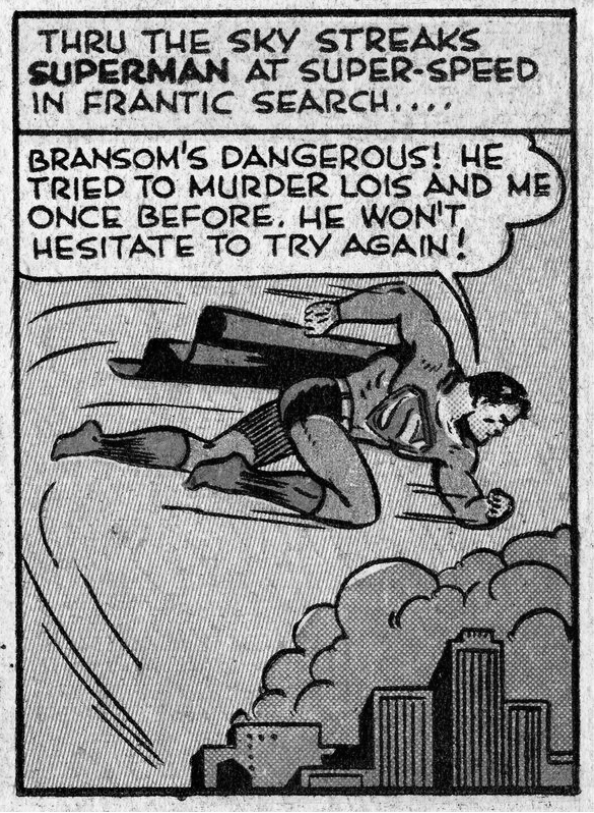
\includegraphics[width=\textwidth]{Figuras/superman.png}
            \caption{Imagen original.} 
         \end{subfigure}
         \begin{subfigure}[h]{0.49\linewidth}
            \centering
            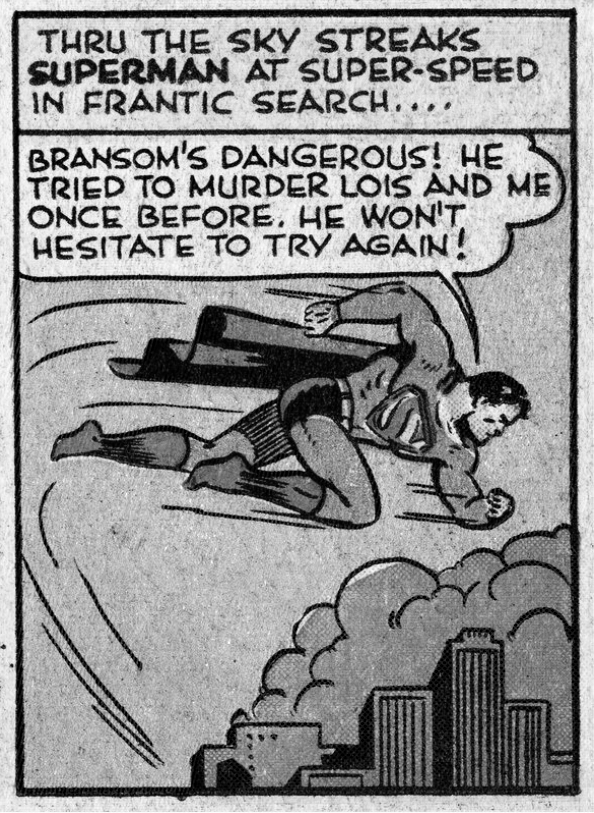
\includegraphics[width=\textwidth]{Figuras/Inverse FFT of superman_process.png}
            \caption{Imagen procesada.}
         \end{subfigure}
    \caption{Comparación imagen original de Superman (a) con la imagen procesada (b) en el espacio de frecuencias sin las componentes periódicas en la textura.}
    \label{fig:superman}
\end{figure}


\begin{figure}[h]
    \centering
         \begin{subfigure}[h]{0.49\linewidth}
            \centering
            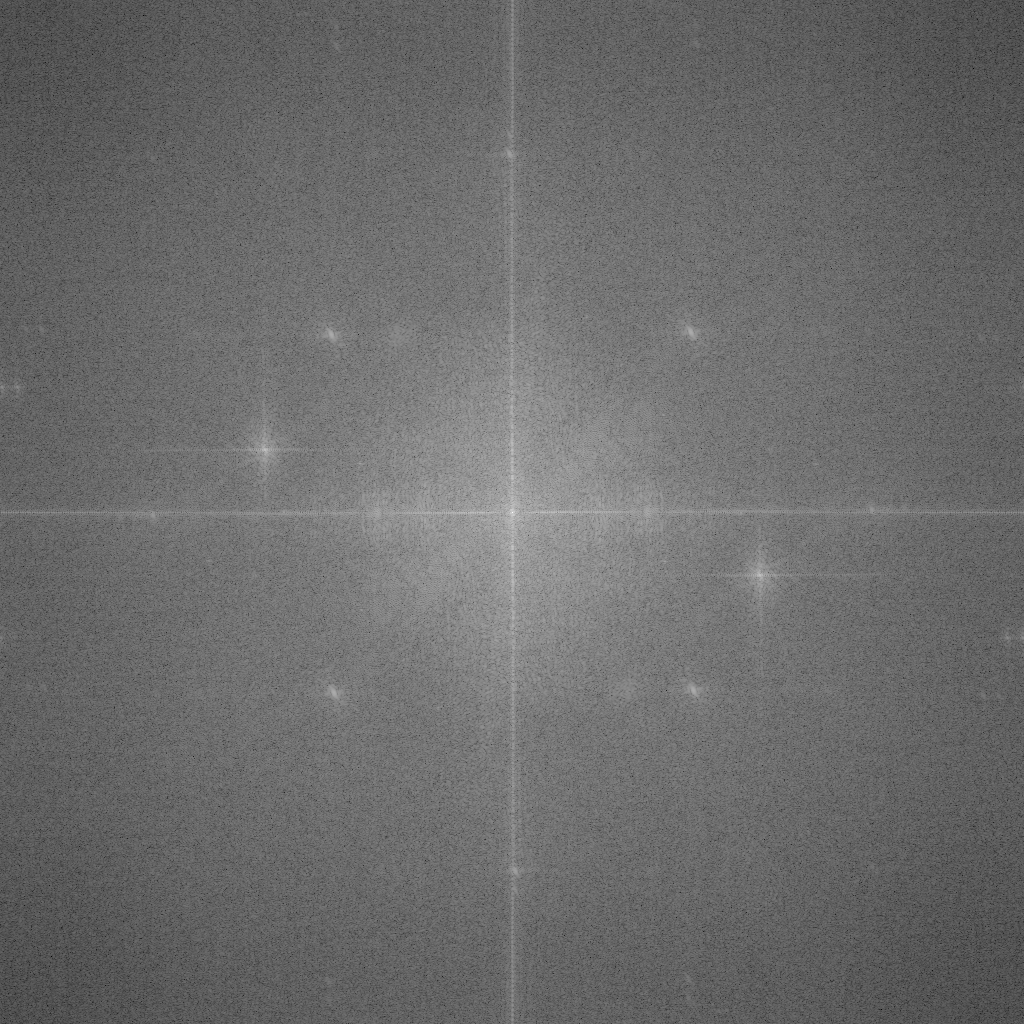
\includegraphics[width=\textwidth]{Figuras/FFT of superman.png}
            \caption{FFT de Superman. \\
            $~$} 
         \end{subfigure}
         \begin{subfigure}[h]{0.49\linewidth}
            \centering
            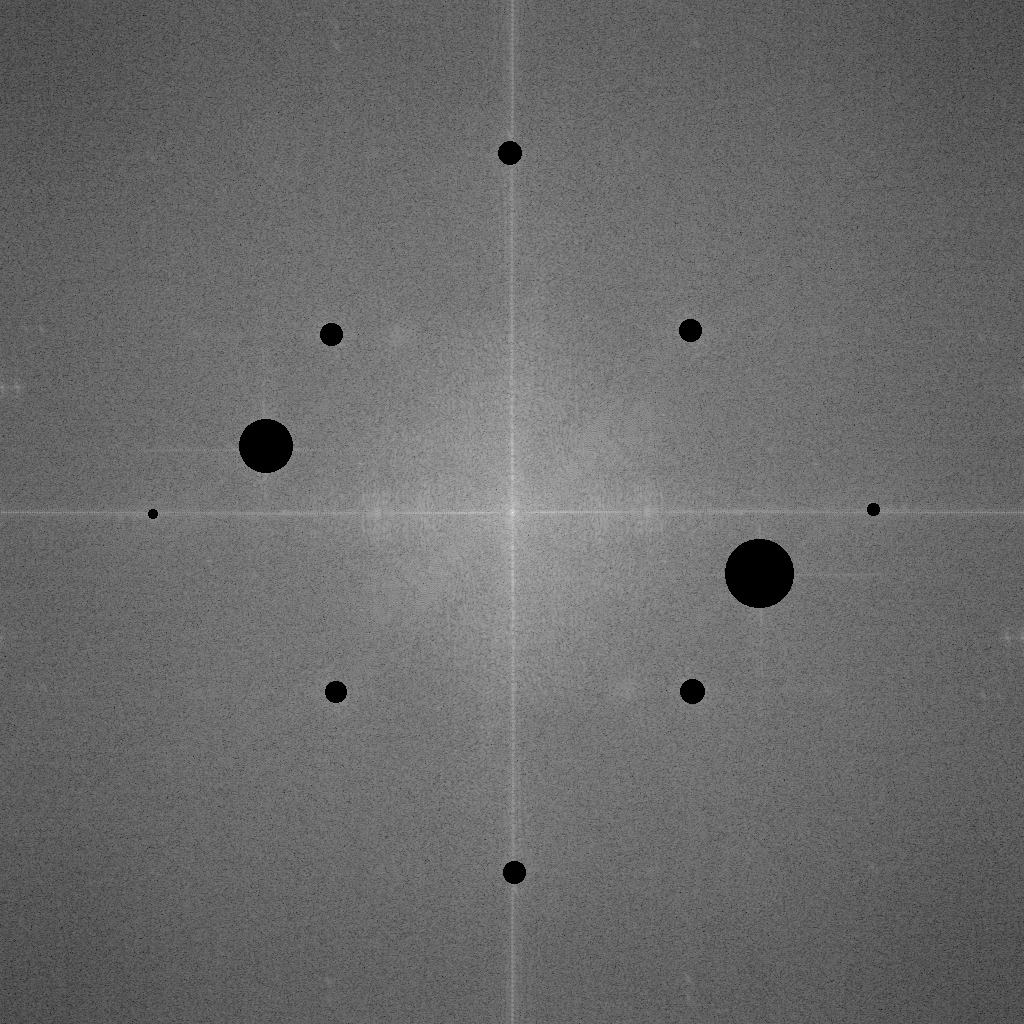
\includegraphics[width=\textwidth]{Figuras/FFT of superman_process.png}
            \caption{FFT de superman procesada.}
         \end{subfigure}
    \caption{Transformada de Fourier rápida de Superman (a). Transformada de Fourier rápida sin las componentes periódicas. En el espacio de frecuencias las componentes periodicas se manifiestan como puntos de alta intensidad.}
    \label{fig:supermanfft}
\end{figure}

\section{Filtros Unsharp y Highboost\label{sec:ej6}}

\vspace{0.3cm}

Los filtros Unsharp y Highboost son filtros que se utilizan para resaltar los bordes de una imagen, se definen de la siguiente manera: Sea $f(x,y)$ la imagen original con ruido, $\tilde{f}(x,y)$ la imagen original luego de aplicarle un filtro pasabajos y $g(x,y)$ la imagen resultante, entonces los filtros se definen como
\begin{itemize}
    \item Unsharp: $g(x,y) = f(x,y) - \tilde{f}(x,y)$
    \item Highboost: $g(x,y) = A~f(x,y) - \tilde{f}(x,y)$
\end{itemize}
donde $A$ es la intensidad del filtro High-boost y vemos que para $A=1$ el filtro High-boost es equivalente al filtro Unsharp. Se tomó la imagen A y se le agregó ruido gaussiano con desvio estándar $\sigma = 5$. Luego, se aplicaron los filtros Unsharp y Highboost utilizando como filtro pasa bajo promedio con un kernel de $7\times7$. Los resultados se muestran en la Fig. \ref{fig:highunsharp}. Se observa que ambos filtros resaltan los bordes de la imagen y amplifican el ruido, lo cual es esperable para este tipo de filtro que escencialmente se comportan como pasa altos. Se puede ver que el filtro Highboost con $A=2$ resalta los bordes, conservando mejor la imagen original. En la Fig. \ref{fig:plot_highboost} se grafica la media cuadrática de la resta entre la imagen con el filtro High-boost y la imagen original sin ruido en función de la intensidad del parámetro $A$. Se observa que $A=2$ es el valor óptimo para resaltar los bordes de la imagen alejandose lo menos posible (en media) de la imagen original.

\begin{figure}[h]
    \centering
         \begin{subfigure}[h]{0.32\linewidth}
            \centering
            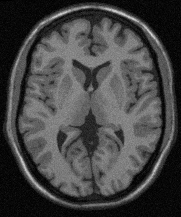
\includegraphics[width=\textwidth]{Figuras/ImagenA.png}
            \caption{ImagenA Original.} 
         \end{subfigure}
         \begin{subfigure}[h]{0.32\linewidth}
            \centering
            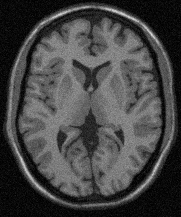
\includegraphics[width=\textwidth]{Figuras/ImagenA_noise=5.png}
            \caption{ImagenA con ruido.} 
         \end{subfigure}
         \begin{subfigure}[h]{0.32\linewidth}
            \centering
            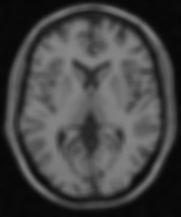
\includegraphics[width=\textwidth]{Figuras/ImagenA_noise=5_filter_7x7.png}
            \caption{ImagenA con ruido filtrada.} 
         \end{subfigure}
         \begin{subfigure}[h]{0.32\linewidth}
            \centering
            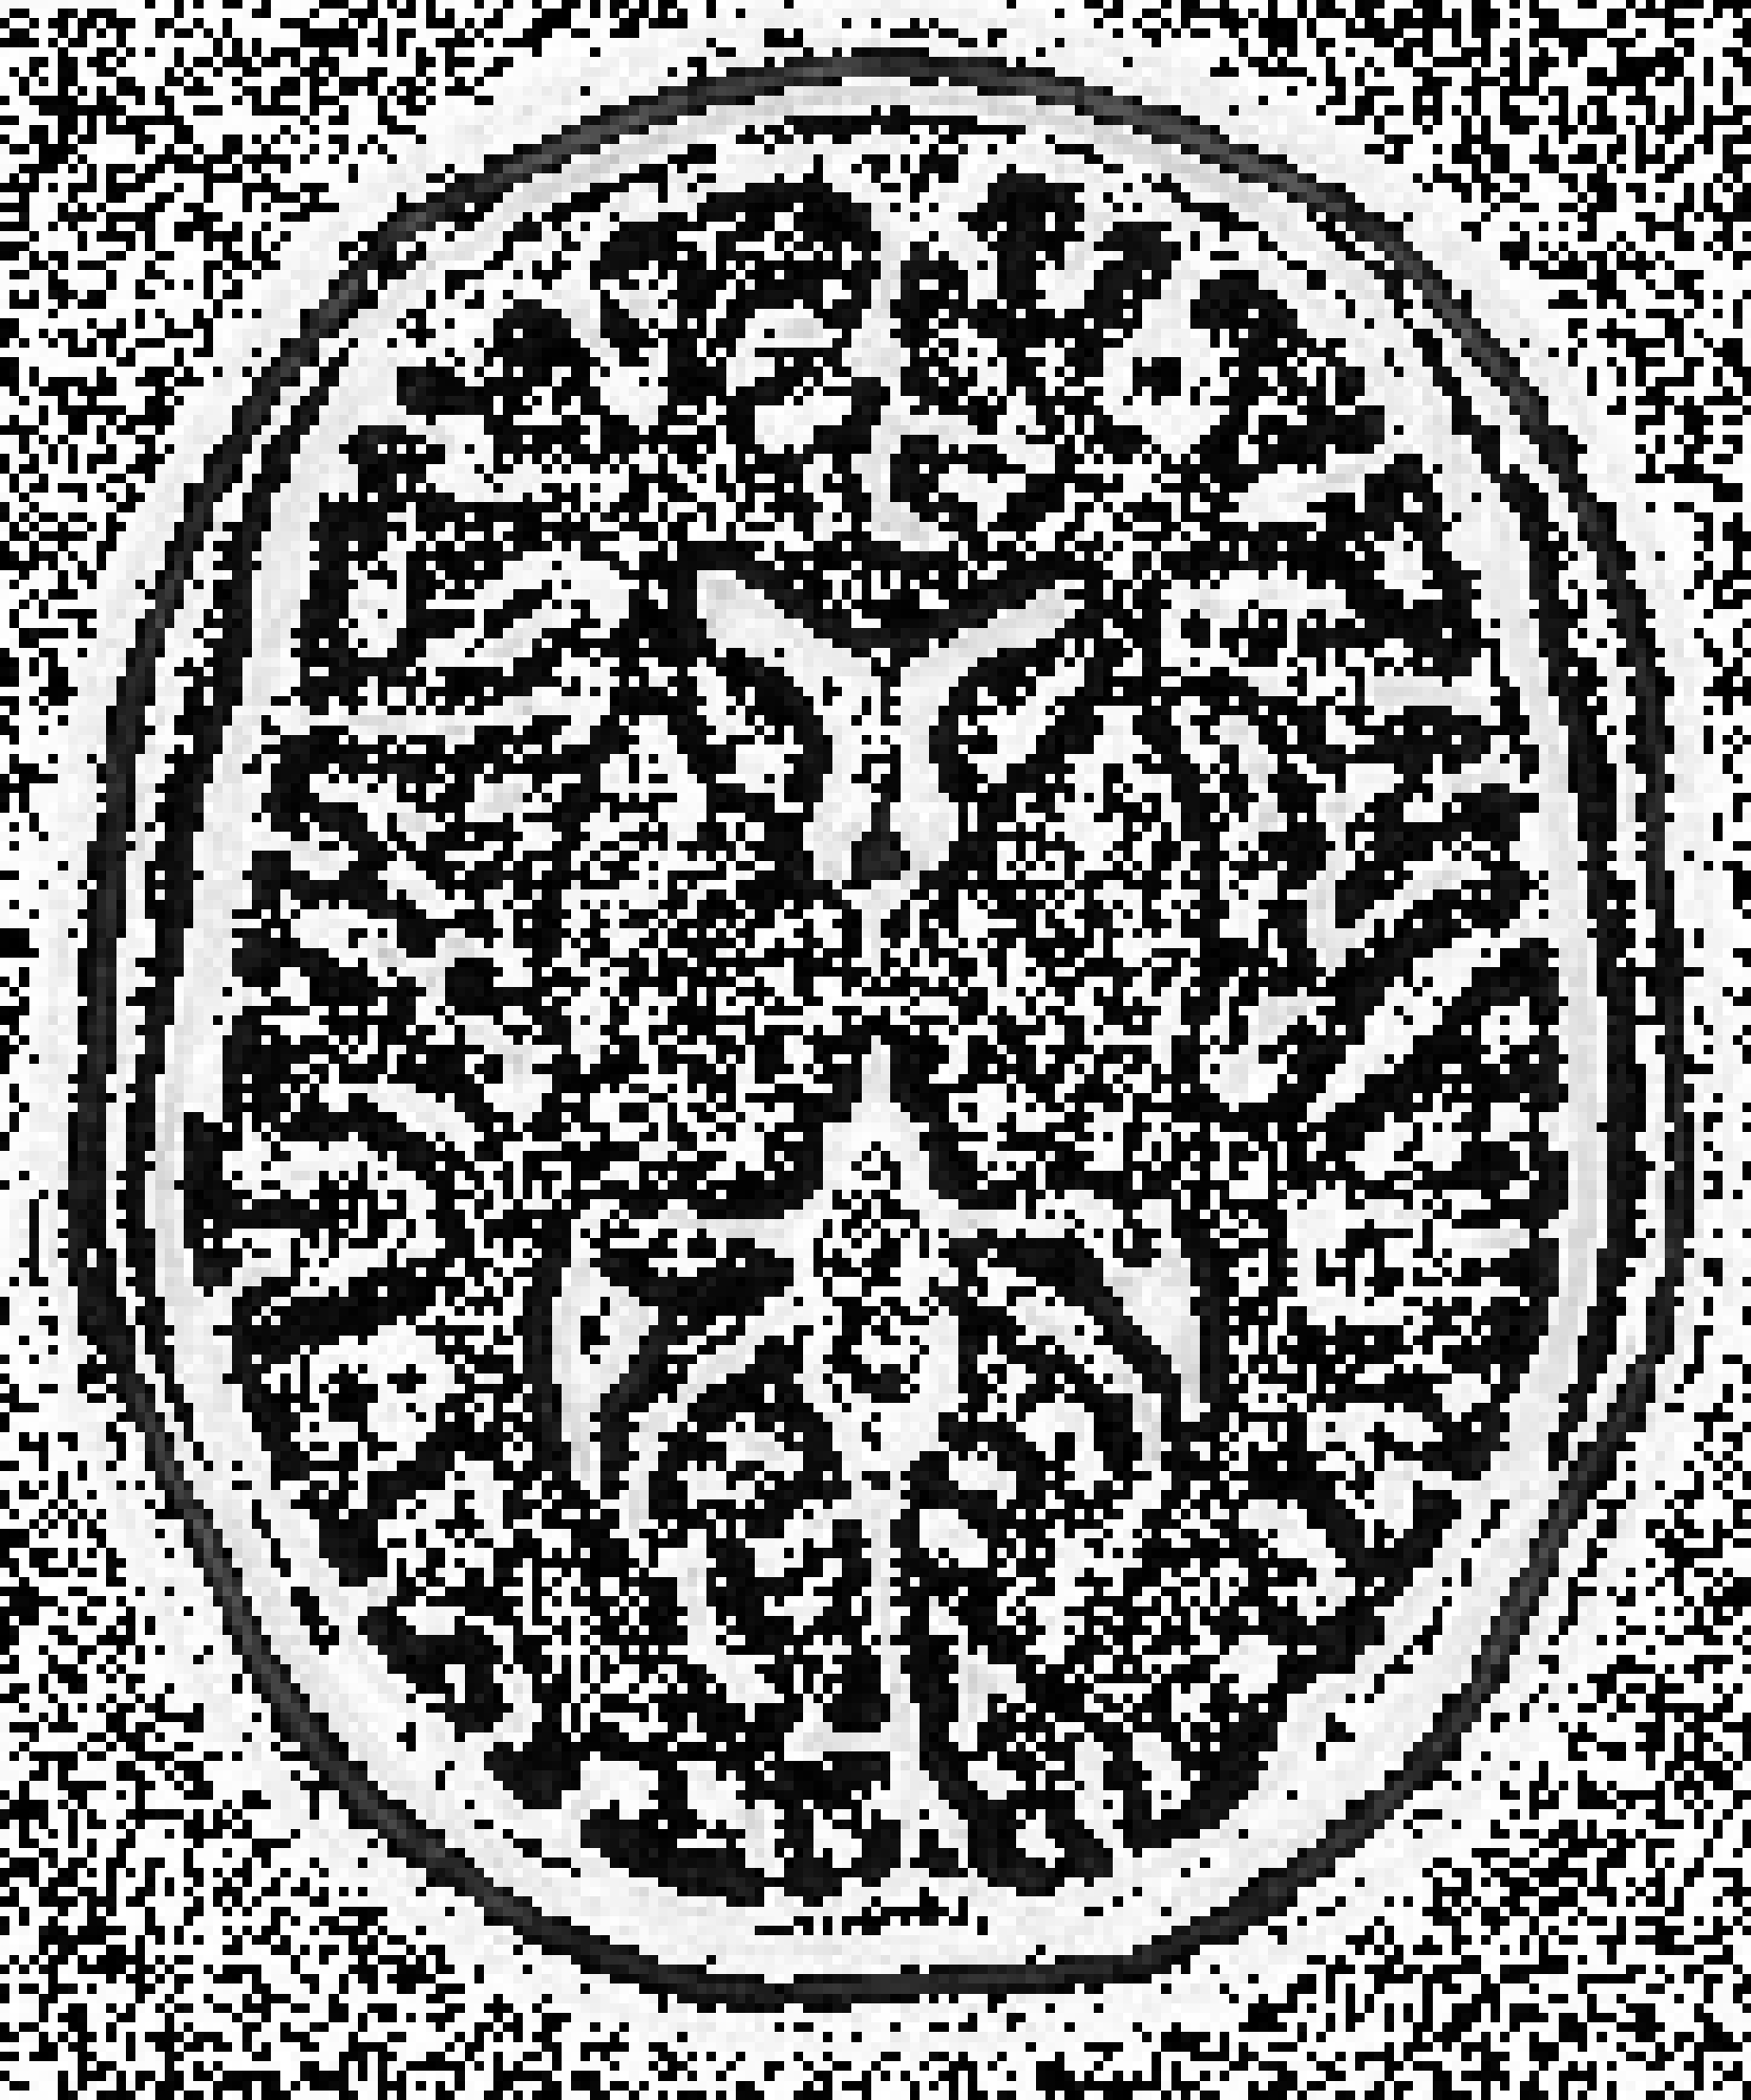
\includegraphics[width=\textwidth]{Figuras/unsharp.png}
            \caption{Filtro Unsharp.} 
         \end{subfigure}
         \begin{subfigure}[h]{0.32\linewidth}
            \centering
            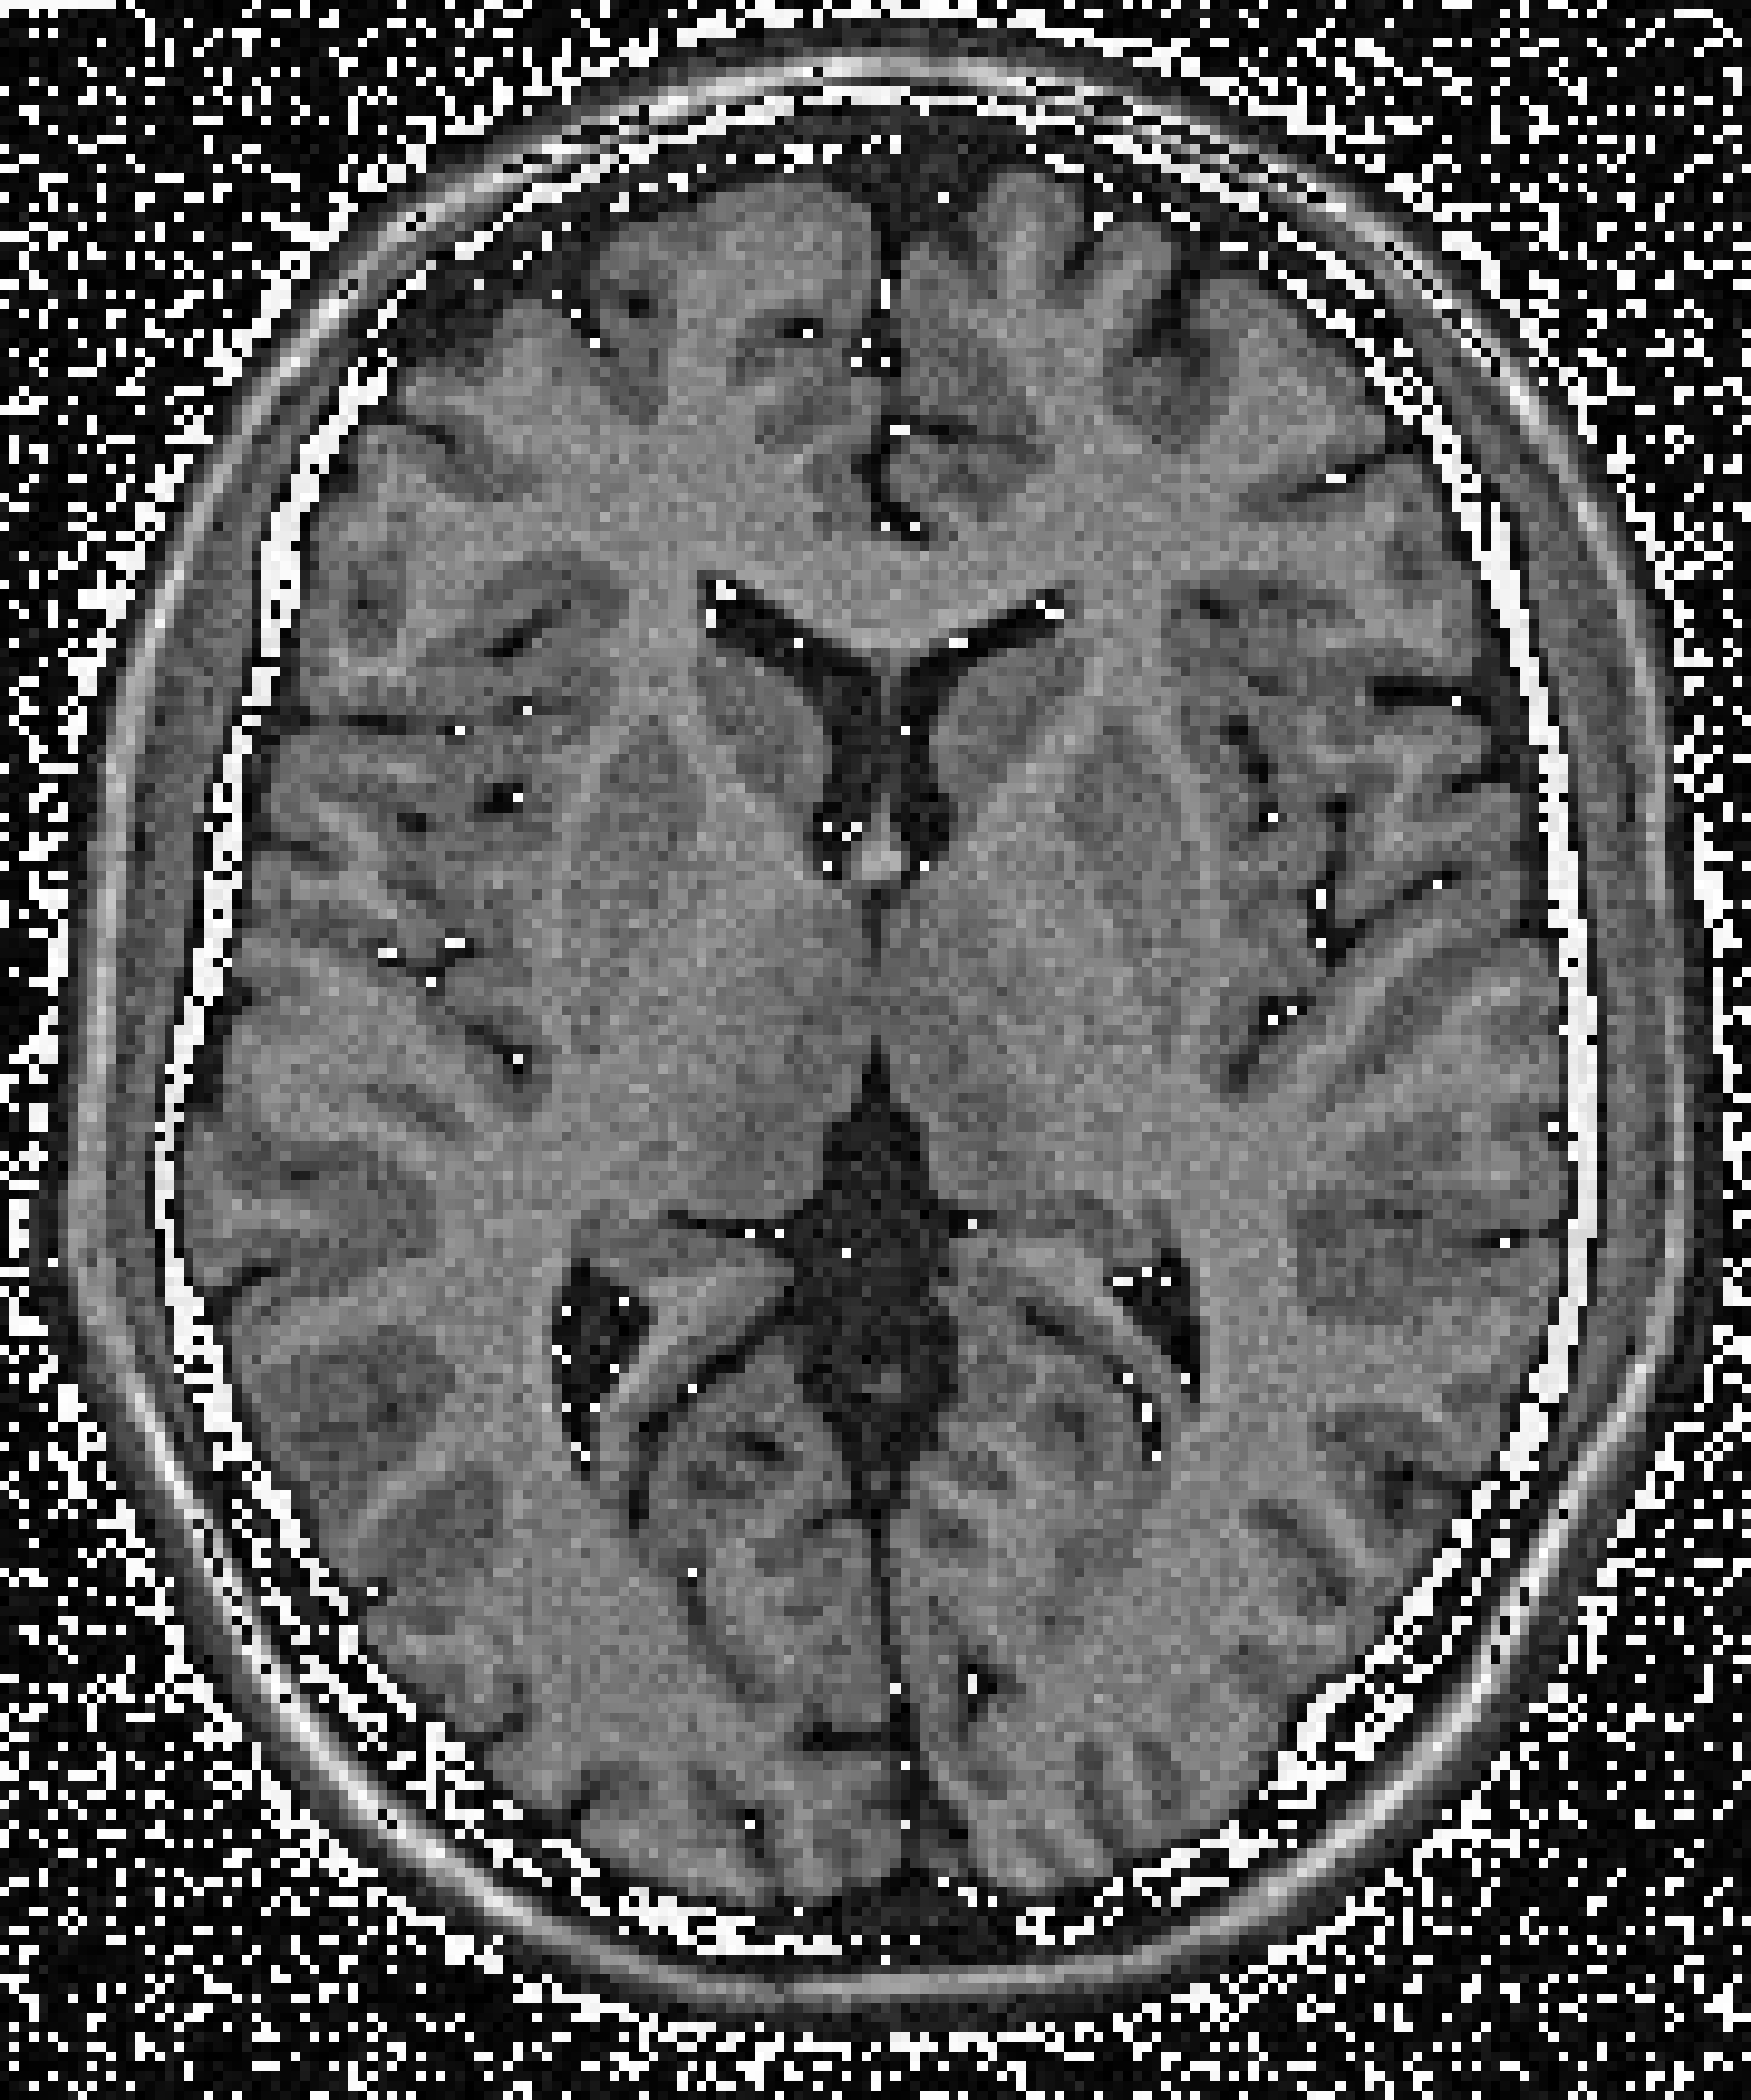
\includegraphics[width=\textwidth]{Figuras/highboost_A=2.png}
            \caption{Filtro Highboost con $A=2$.} 
         \end{subfigure}
         \begin{subfigure}[h]{0.32\linewidth}
            \centering
            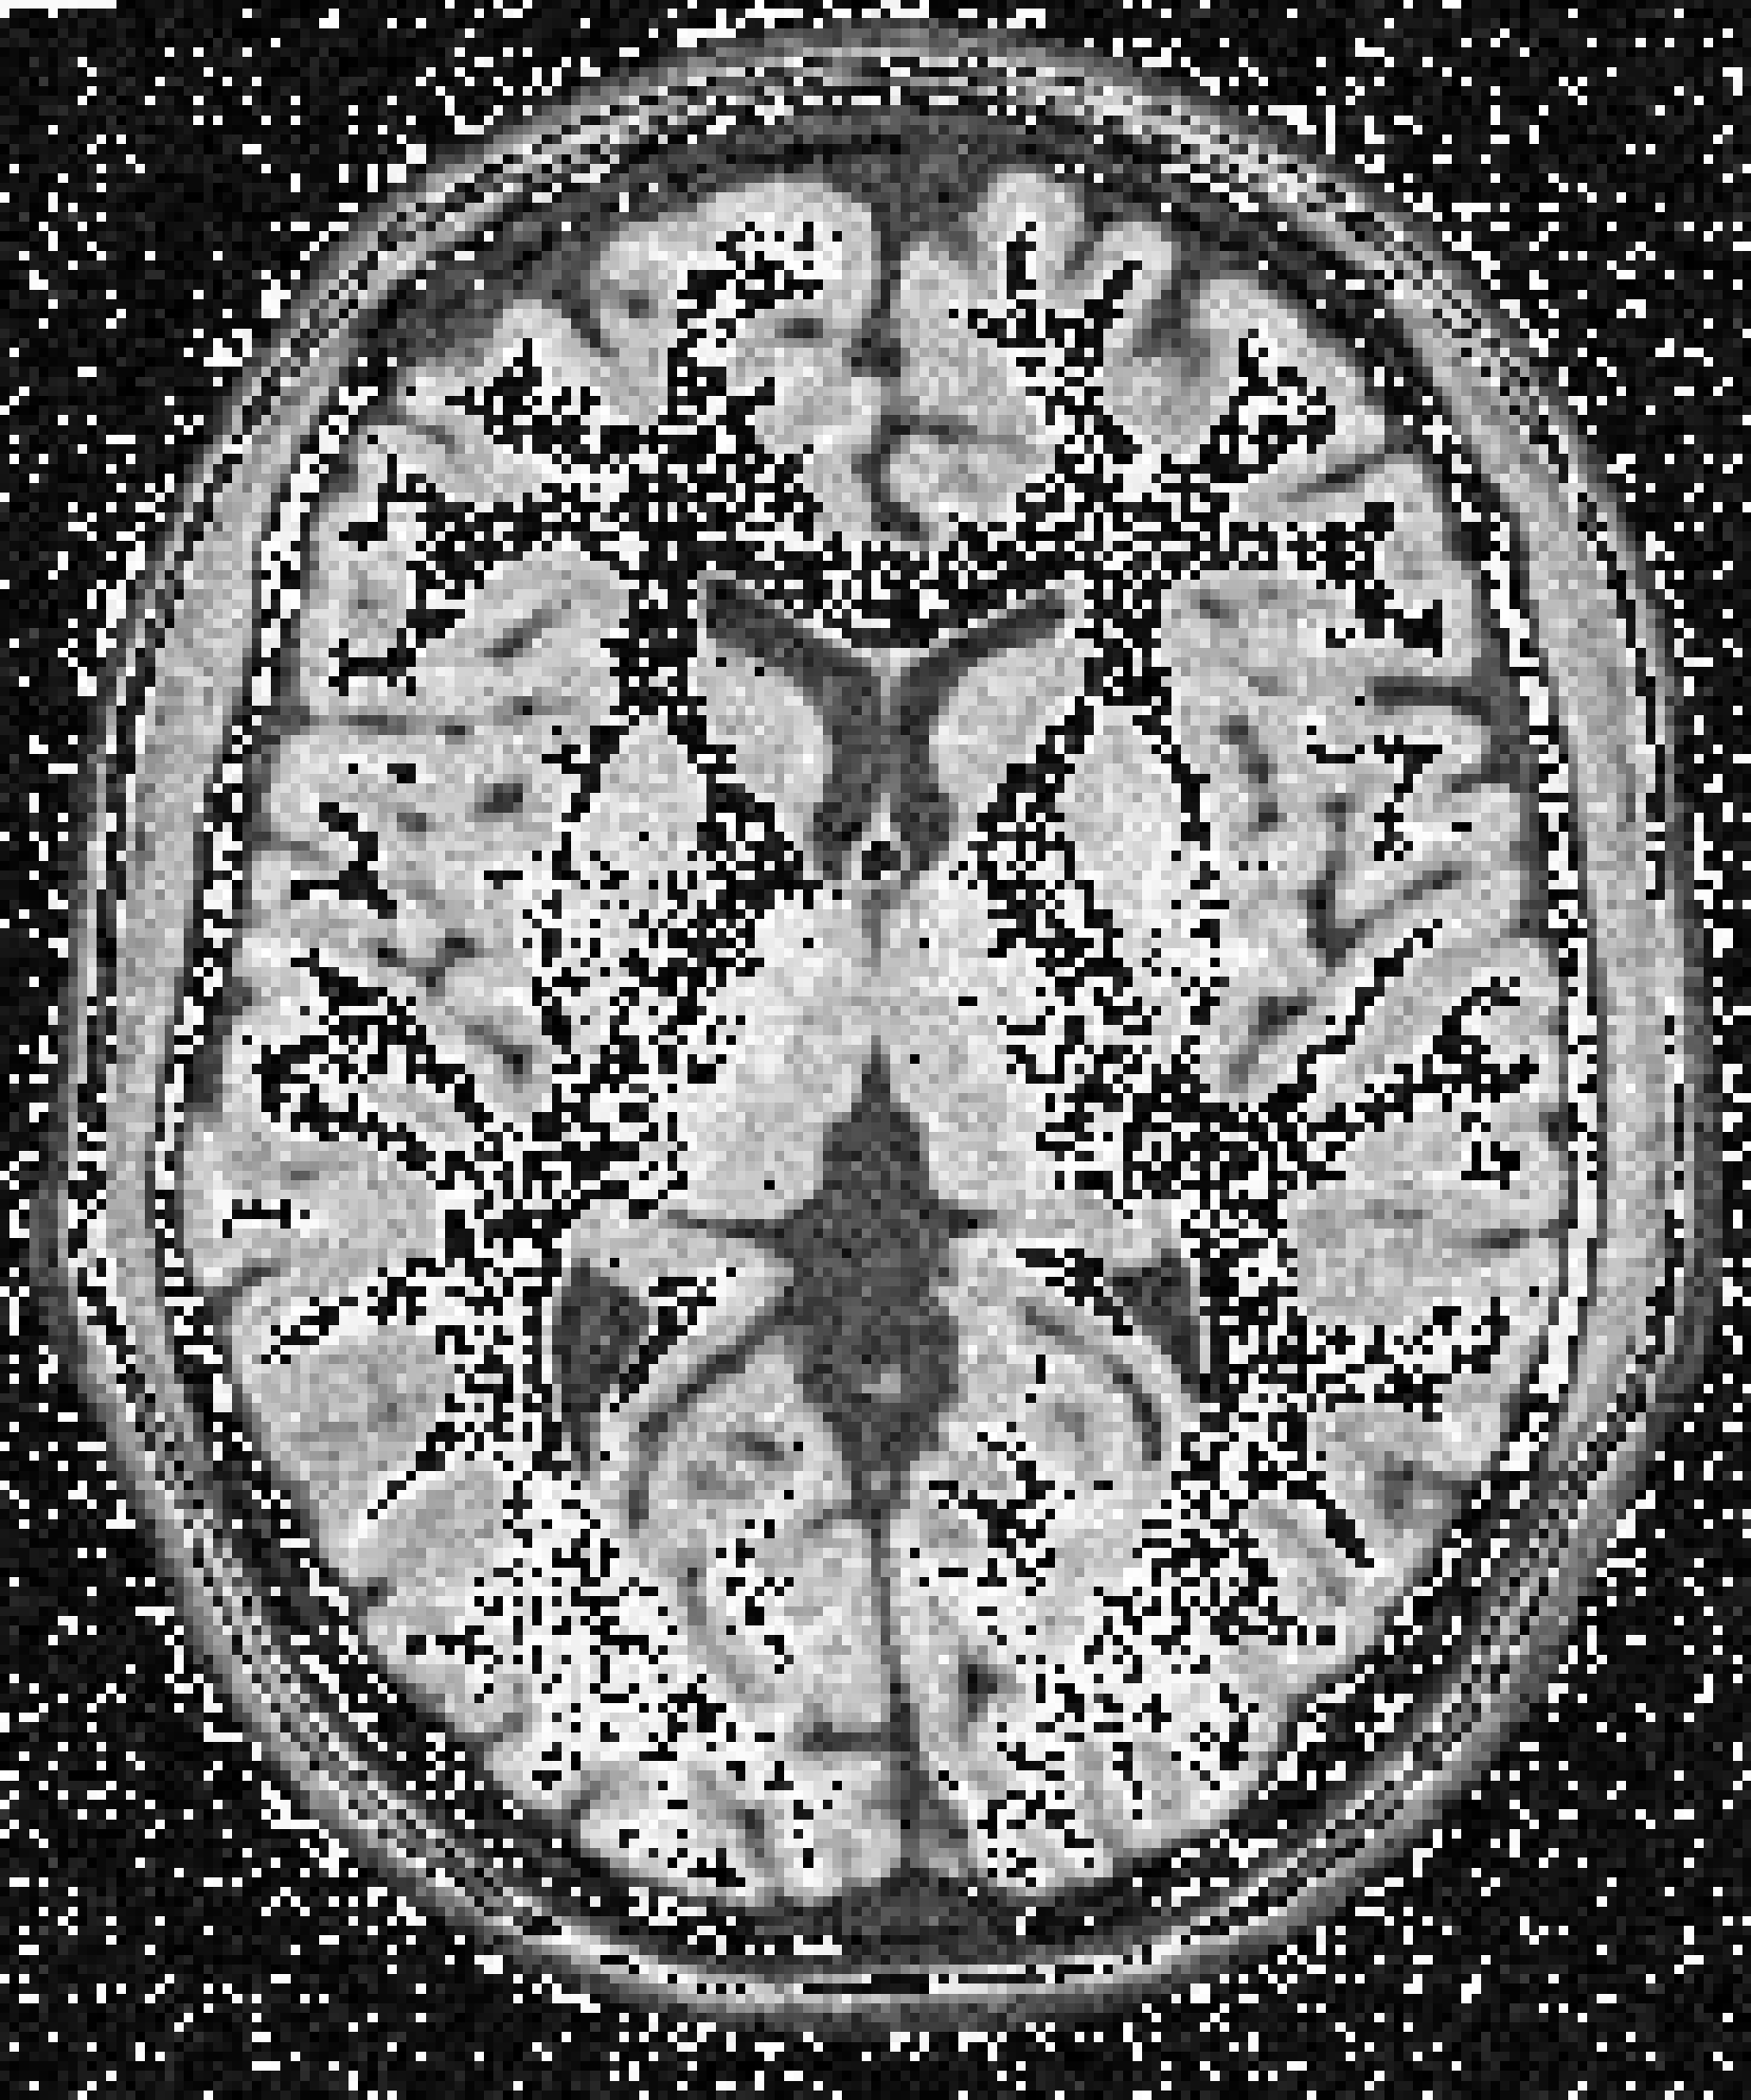
\includegraphics[width=\textwidth]{Figuras/highboost_A=3.png}
            \caption{Filtro Highboost con $A=3$.} 
         \end{subfigure}
    \caption{Filtraos Unsharp y Highboost aplicados a la imagenA con ruido gaussiano con desvio estandar $\sigma =5$.}
    \label{fig:highunsharp}
\end{figure}

\begin{figure}[h]
    \centering
         \begin{subfigure}[h]{\linewidth}
            \centering
            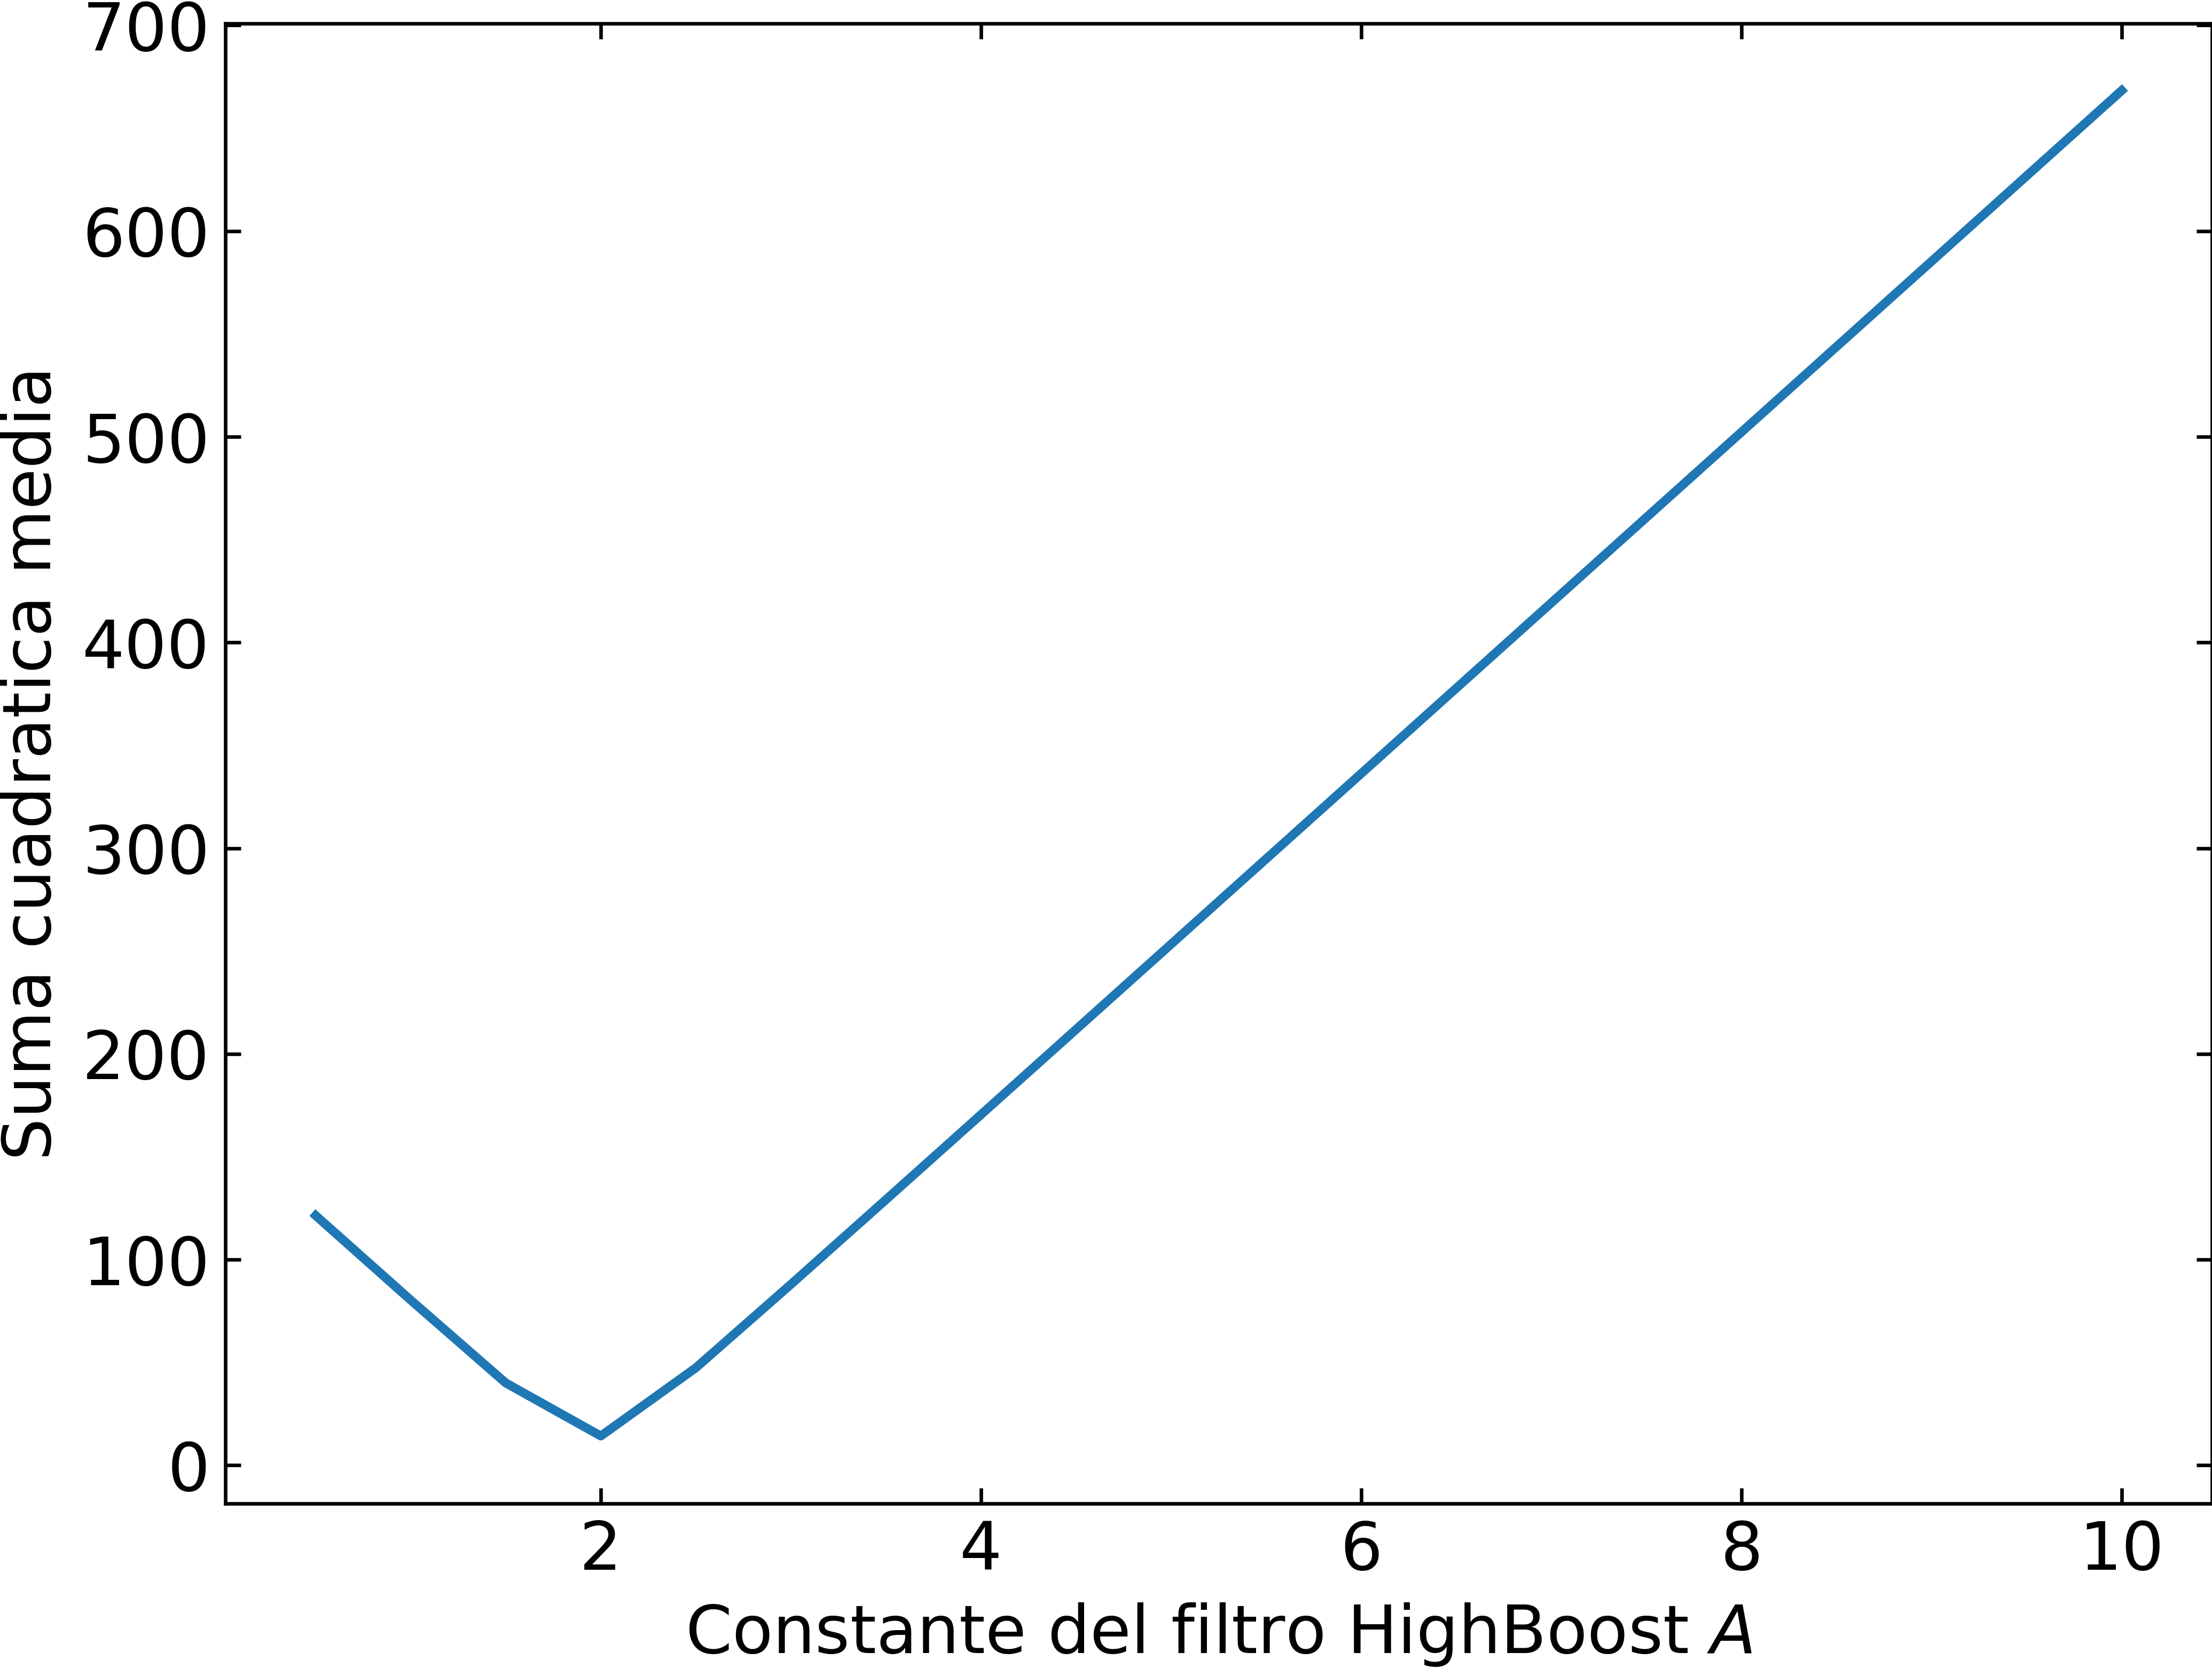
\includegraphics[width=0.7\textwidth]{Figuras/Highboost_plot.png}
            \caption{ImagenA original junto con su histograma de intensidades.} 
         \end{subfigure}
    \caption{Gráfica de la media cuadrática de la diferencia entre la imagen original sin ruido y la imagen filtrada con el filtro High-boost en función del parámetro $A$.}
    \label{fig:plot_highboost}
\end{figure}

\section{Calibración de fantomas\label{sec:ej7}}

\vspace{0.3cm}

Se calcularon las relaciones señal-ruido (SNR) para los cortes 2, 3 y 4 de un fantoma adquiridos con CT HiSpeed. En este caso, se utilizó ImageJ para obtener los histogramas de intensidad de pixel de una región de interés (ROI por sus siglas en inglés) de las imágenes de los fantomas tomadas como se muestra en la Fig. \ref{fig:SNR} para el caso de la imagen AAA0002. La SNR se calcula como 
\begin{equation}
    SNR = \frac{\mu}{\sigma}
\end{equation}
donde $\mu$ es la media de la intensidad de la imagen y $\sigma$ es la desviación estándar en la ROI elegida. En la tabla \ref{tab:SNR} se muestran los valores de $\mu$, $\sigma$ y SNR para cada corte. Se observa que el SNR disminuye a medida que disminuye la corriente del tubo de rayos X. Esto es consistente con lo observado en las imágenes de los cortes, donde se observa que a menor corriente, la imágenes se vuelven más ruidosas.

\begin{figure}[h]
    \centering
         \begin{subfigure}[h]{0.49\linewidth}
            \centering
            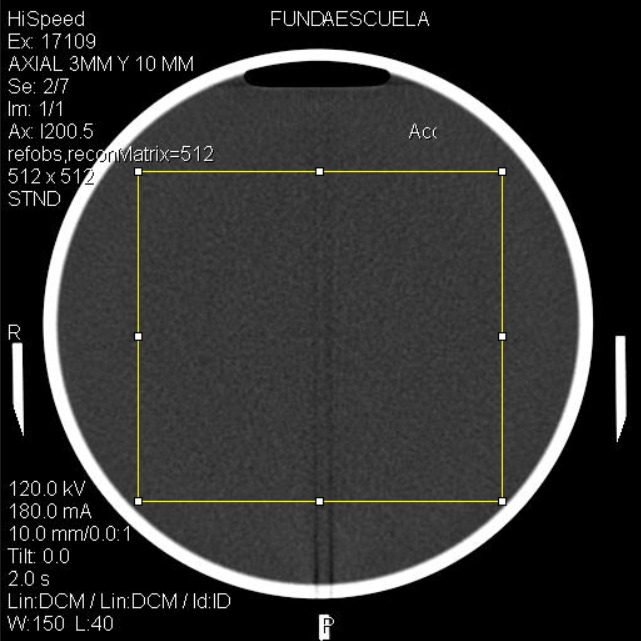
\includegraphics[width=0.7\textwidth]{Figuras/roi_corte2.png}
            \caption{Imagen con la ROI seleccionada. \\
            $~$} 
         \end{subfigure}
         \begin{subfigure}[h]{0.49\linewidth}
            \centering
            \includegraphics[width=\textwidth]{Figuras/hist_corte2.png}
            \caption{Histograma de intensidades.}
         \end{subfigure}
    \caption{Estimación de la SNR para la imagen AAA0002.}
    \label{fig:SNR}
\end{figure}

\begin{table}[h]
    \centering
    \begin{tabular}{c||c|c|c|c}
    \hline
    Corte & Corriente (mA) & $\mu$     & $\sigma$ & SNR \\ \hline
    2     & 180.0          & 57.074 & 4.422 & 12.907   \\ \hline
    3     & 100.0          & 56.722 & 5.769 & 9.832   \\ \hline
    4     & 60.0           & 56.728 & 7.286 & 7.786   \\ \hline
    \end{tabular}
    \caption{Tabla de corriente, media, desviación estándar y SNR para las imágenes AAA000x siendo x el corte.} \label{tab:SNR}
\end{table}

Por otro lado, se midieron el ancho total a media altura (FWHM por sus siglas en inglés) del perfil de intensidad del punto del fantoma para los cortes 11, 12, 13 y 14. En la Fig. \ref{fig:FWHM}a se muestra el corte 11 y la ROI sobre el cual se obtuvo el perfil de intensidad y en la Fig. \ref{fig:FWHM}b se muestra el FWHM para dicho perfil de intensidad. En la tabla \ref{tab:FWHM} se muestran los valores de FWHM para cada corte.

\begin{table}[h]
    \centering
    \begin{tabular}{c||c}
    \hline
    Corte & FWHM  \\ \hline
    11    & 5.720   \\ \hline
    12    & 2.967   \\ \hline
    13    & 6.267   \\ \hline
    14    & 4.425   \\ \hline
    \end{tabular}
    \caption{Tabla FWHM para las imágenes AAA00xx siendo x el corte.} 
    \label{tab:FWHM}
\end{table}

\begin{figure}[h]
    \centering
         \begin{subfigure}[h]{0.49\linewidth}
            \centering
            \includegraphics[width=0.8\textwidth]{Figuras/roi_zoom_corte11.png}
            \caption{Imagen con la ROI seleccionada. \\
            $~$} 
         \end{subfigure}
         \begin{subfigure}[h]{0.49\linewidth}
            \centering
            \includegraphics[width=1.1\textwidth]{Figuras/profile_corte11.png}
            \caption{Perfil de intensidad.}
         \end{subfigure}
    \caption{Estimación del FWHM para la imagen AAA0011.}
    \label{fig:FWHM}
\end{figure}


%\begin{figure}[h]
%    \centering
%         \begin{subfigure}[h]{0.9\linewidth}
%            \centering
%            \includegraphics[width=\textwidth]{Figuras/profile_corte12.png}
%            \caption{ImagenA original junto con su histograma de intensidades.} 
%         \end{subfigure}
%    \caption{}
%    \label{fig:corte12}
%\end{figure}

\centerline{\rule{0.95\linewidth}{0.6pt}}

% Bibliography
%\renewcommand*{\bibfont}{\normalsize}
%\bibliography{Redes}

% Full bibliography added automatically for Optics Letters submissions; the following line will simply be ignored if submitting to other journals.
% Note that this extra page will not count against page length
%\bibliographyfullrefs{Redes}

\clearpage

\begin{onecolumn} % Activa una sola columna para el apéndice
\appendix
\section{Apéndice \label{codigo}}
\scriptsize
\begin{lstlisting}[style=mystyle]
    import cv2
    import sys 
    import numpy as np
    import matplotlib.pyplot as plt
    import os.path
    
    def read_pgm_file(file_name):
    
        data_dir = os.path.dirname(os.path.abspath(__file__))
    
        # Test if file exists
        file_path = os.path.join(data_dir, file_name)
        assert os.path.isfile(file_path), 'file \'{0}\' does not exist'.format(file_path)
    
        img = cv2.imread(file_name,flags=cv2.IMREAD_GRAYSCALE)
    
        if img is not None:
            print('img.size: ', img.size)
        else:
            print('imread({0}) -> None'.format(file_path))
    
        return img
    
    def save_img_hist(im,filename):
        
        vmin = np.amin(im)
        vmax = np.max(im)
        print("Intensity Min: {}  Max:{}".format(vmin,vmax))
    
        L = vmax - vmin
        print("Number of Levels: {}".format(L))
        fig = plt.figure(figsize=(12,5))
        ax1 = plt.subplot(1, 2, 1)
        ax2 = plt.subplot(1, 2, 2)
    
        # imgplot = plt.imshow(im/np.amax(im))
        imgplot = ax1.imshow(im,cmap='gray', vmin=vmin, vmax=vmax)
        fig.colorbar(imgplot, ax=ax1)
        #ax1.tick_params(direction='in', top=True, right=True, left=True, bottom=True)
        ax1.tick_params(axis='x', rotation=0, labelsize=15, color='black')
        ax1.tick_params(axis='y', labelsize=15, color='black')
        # cv2.imshow(infile,img)
        # cv2.waitKey(0)
    
        hist, bin_edges = np.histogram(im.ravel(),bins=L)
        ax2.bar(bin_edges[:-1], hist, alpha=1, color='b')
        ax2.set_xlabel(r"Intensidad de pixel", fontsize=15)
        ax2.set_ylabel(r"Número de píxeles", fontsize=15)
        ax2.tick_params(direction='in', top=True, right=True, left=True, bottom=True)
        ax2.tick_params(axis='x', rotation=0, labelsize=15, color='black')
        ax2.tick_params(axis='y', labelsize=15, color='black')
        ax2.set_xlim(-5, 260)
        #ax2.set_ylim(0, 1000)
    
        #x1 = rmin  # Punto inicial en el eje x
        #x2 = rmax  # Punto final en el eje x
        #y1 = 0  # Punto inicial en el eje y (puedes ajustar este valor según tu necesidad)
        #y2 = 255  # Punto final en el eje y (puedes ajustar este valor según tu necesidad)
    
        #Agrega la recta al segundo subplot (ax2)
        #ax2.plot([x1, x2], [y1, y2], color='r', linestyle='-', linewidth=2)  # Trama la línea recta
    
        fig.savefig(f"{filename}_hist.pdf")
        fig.savefig(f"{filename}_hist.png", dpi=600)
        #plt.show()
    
    def save_img(im,filename):
        
        vmin = np.amin(im)
        vmax = np.max(im)
        print("Intensity Min: {}   Max:{}".format(vmin,vmax))
    
        L = vmax - vmin
        print("Number of Levels: {}".format(L))
    
        fig, ax = plt.subplots()
        imgplot = ax.imshow(im,cmap='gray', vmin=vmin, vmax=vmax)
        ax.axis('off')
    
        fig.savefig(f"{filename}.pdf", pad_inches = 0,bbox_inches='tight')
        fig.savefig(f"{filename}.png", dpi=600, pad_inches = 0, bbox_inches='tight')
        print("Size of image: {}".format(im.shape))
        #plt.show()
    
    def SemilinearTrans_pgm_file(im,rmin,rmax):
        Imin = 0
        Imax = 255
        a = (Imax - Imin)/(rmax-rmin)
        b = Imin - a*rmin  
        imout = a*im + b
    
        imout = np.where(imout < Imin, Imin, imout)
        imout = np.where(imout > Imax, Imax, imout)
        imout = imout.astype(int)
        return imout
    
    def Equalize_pgm_file(im):
        imout = im 
        vmin = np.amin(im)
        vmax = np.max(im)
        L = vmax - vmin
        hist, bin_edges = np.histogram(im.ravel(),bins=L)
        hist_norm = hist / np.sum(hist)  #Normaliza el histograma
    
        suma = 0
        for i in range(0,im.shape[0]):
            for j in range(0,im.shape[1]):
                suma = 0
                for e in range(0,im[i,j]):
                   suma += hist_norm[e]
                imout[i,j] = 255*suma
    
        imout = imout.astype(int)
        return imout
    
    def Trans_binary(im):
        imout=np.where(im<128,255,0)
        imout = imout.astype(int)
        return imout
    
    def Trans_exponential(im,gamma):
        imout=im
        imout=255*(imout/im.max())**gamma
        imout=imout.astype(int)
        return imout
    
    def sustraction(im1,im2):
        imout = im1 - im2
        return imout
    
    def interpolate_nn(im,f):
        Nx, Ny = im.shape[0],im.shape[1]
        Mx=int(f*Nx)
        My=int(f*Ny)
        imout=np.ndarray((Mx,My), dtype=int)
    
        for x in range(Mx):
            for y in range(My):
                imout[x][y]=im[round(x*Nx/Mx)%Nx][round(y*Ny/My)%Ny]
    
        return imout
    
    def interpolate_bilinear(im, output_width, output_height):
    
        # Calculate scaling ratios
        old_height, old_width = im.shape[:2]
        x_ratio = old_width / output_width
        y_ratio = old_height / output_height
    
        # Create new image array
        new_img = np.zeros((output_height, output_width), dtype=np.uint8)
    
        # Perform bilinear interpolation
        for y in range(output_height):
            for x in range(output_width):
                x_original = x * x_ratio
                y_original = y * y_ratio
                x0 = int(x_original)
                y0 = int(y_original)
                x1 = min(x0 + 1, old_width - 1)
                y1 = min(y0 + 1, old_height - 1)
    
                Q11 = im[y0, x0]
                Q21 = im[y1, x0]
                Q12 = im[y0, x1]
                Q22 = im[y1, x1]
    
                x_weight = x_original - x0
                y_weight = y_original - y0
    
                R1 = Q11 * (1 - x_weight) + Q12 * x_weight
                R2 = Q21 * (1 - x_weight) + Q22 * x_weight
    
                P = R1 * (1 - y_weight) + R2 * y_weight
    
                new_img[y, x] = P
    
        return new_img
    
    def high_boost(im,im_filtered,A):
        imout = A*im - im_filtered
        return imout
    
    def unsharp(im,im_filtered):
        imout = im - im_filtered
        return imout
    
    if __name__ == "__main__":
        
        if(len(sys.argv)<3):
            print("Usage: python read-write-pgm.py [infile.pgm] [outfile.pgm]")
            exit(1)
    
        infile1 = sys.argv[1]
        outfile1 = sys.argv[2]
        #infile2 = sys.argv[3]
        #outfile2 = sys.argv[4]
        
        img1 = read_pgm_file(infile1)
        #img2 = read_pgm_file(infile2)
        im1 = np.array(img1)
        #im2 = np.array(img2)
        
        #Brute image 
        print("\n Brute image:")
        print("Size of image 1: {}".format(im1.shape))
        #print("Size of image 2: {}".format(im2.shape))
        save_img_hist(im1,"ImageA_brute",0,150)
    
        #Semilinear transformation for different rmin values
        print("\n Semilinear transformation")
        img = read_pgm_file(infile1)
        im = np.array(img)
        rmax = 150 # 25, 62 , 113 ,150
        rmin = 113 # 0, 25 , 62 , 113 
        imout = SemilinearTrans_pgm_file(im,rmin,rmax)
        print("Size of image: {}".format(imout.shape))
        save_img_hist(imout,"ImageA_"+str(rmin)+"_"+str(rmax))
        save_img(imout,"ImageA_"+str(rmin)+"_"+str(rmax))
    
        #Equalize image
        print("\n Equalize image")
        imout = Equalize_pgm_file(im1)
        save_img_hist(imout,"ImageA_EQ")    
        save_img(imout,"ImageA_EQ")    
        #cv2.imwrite(outfile1,imout,[cv2.IMWRITE_PXM_BINARY,0])
    
        #Transformación binaria
        print("\n Transformación binaria")
        imout = Trans_binary(im1)
        save_img(imout,f"ImageA_binary")
        #cv2.imwrite(outfile1,imout,[cv2.IMWRITE_PXM_BINARY,0])
    
        #Transformación exponencial
        print("\n Transformación exponencial")
        gamma = 0.5
        imout = Trans_exponential(im1,gamma)
        save_img(imout,f"ImageA_exp_gamma={gamma}")
        #cv2.imwrite(outfile1,imout,[cv2.IMWRITE_PXM_BINARY,0])
        
        #Interpolate nn
        f = 0.25
        print("\n Interpolate NN")
        imout = interpolate_nn(im1,f)
        save_img(imout,f"Interpolate_nn_f={f}")
    
        #Interpolate bilinear
        #f = 0.25
        print("\n Interpolate bilinear")
        imout = interpolate_bilinear(im1, int(f* im1.shape[0]), int(f* im1.shape[1]))
        save_img(imout,f"Interpolate_bilinear_f={f}")
        cv2.imwrite(outfile1,imout,[cv2.IMWRITE_PXM_BINARY,0])
    
        #Sustraction
        print("\n Sustraction")
        imout = sustraction(im1,im2)
        save_img(imout,f"sustraction_exp_gamma=0.5")
        cv2.imwrite(outfile1,imout,[cv2.IMWRITE_PXM_BINARY,0])
    
        #Unsharp filter
        print("\n Unsharp filter")
        imout1 = unsharp(im1,im2)
        imout1 = np.array(imout1)
        print("Size of image 1: {}".format(imout1.shape))
        save_img(imout1,"unsharp")
    
        #HighBoost filter
        print("\n HighBoost filter ")
        A=3
        imout2 = high_boost(im1,im2,A)
        imout2 = np.array(imout2)
        print("Size of image 2: {}".format(imout2.shape))
        save_img(imout2,f"highboost_A={A}")
    
        #High Boost filter plot
        print("\n High Boost filterplot")
        A = np.arange(0.5, 10.5, 0.5)
        S = ([])
    
        for a in A:
            imout2 = high_boost(im1,im2,a)
            im_sust = sustraction(imout2,im1)
            matriz_cuadrada = np.square(im_sust)
            suma_total = np.sum(matriz_cuadrada)
            media = np.sqrt(suma_total / im_sust.size)
            S = np.append(S, media)
            #imout2 = np.array(imout2)
            #print("Size of image 1: {}".format(imout2.shape))
            #imout2 = Equalize_pgm_file(imout2)
            #save_img(imout2,f"highboost_A={A}")
            #cv2.imwrite(outfile2,imout2,[cv2.IMWRITE_PXM_BINARY,0])
        
        fig, ax = plt.subplots(figsize=(8, 6))
        ax.plot(A, S, linewidth=2)
        ax.set_xlabel(f"Intensidad del filtro HighBoost $A$", fontsize=15)
        ax.set_ylabel(f"Suma cuadratica media", fontsize=15)
        ax.tick_params(direction='in', top=True, right=True, left=True, bottom=True)
        ax.tick_params(axis='x', rotation=0, labelsize=15, color='black')
        ax.tick_params(axis='y', labelsize=15, color='black')
        #ax.set_xlim(-5, 260)
        #ax2.set_ylim(0, 1000)
        fig.savefig(f"Highboost_plot.pdf", pad_inches = 0,bbox_inches='tight')
        fig.savefig(f"Highboost_plot.png", dpi=600, pad_inches = 0, bbox_inches='tight')
\end{lstlisting}
\end{onecolumn}
\end{document}


